%% Copernicus Publications Manuscript Preparation Template for LaTeX Submissions
%% ---------------------------------
%% This template should be used for copernicus.cls
%% The class file and some style files are bundled in the Copernicus Latex Package, which can be downloaded from the different journal webpages.
%% For further assistance please contact Copernicus Publications at: production@copernicus.org
%% https://publications.copernicus.org/for_authors/manuscript_preparation.html


%% Please use the following documentclass and journal abbreviations for preprints and final revised papers.

%% 2-column papers and preprints
\documentclass[journal abbreviation, manuscript]{copernicus}



%% Journal abbreviations (please use the same for preprints and final revised papers)


% Advances in Geosciences (adgeo)
% Advances in Radio Science (ars)
% Advances in Science and Research (asr)
% Advances in Statistical Climatology, Meteorology and Oceanography (ascmo)
% Aerosol Research (ar)
% Annales Geophysicae (angeo)
% Archives Animal Breeding (aab)
% Atmospheric Chemistry and Physics (acp)
% Atmospheric Measurement Techniques (amt)
% Biogeosciences (bg)
% Climate of the Past (cp)
% DEUQUA Special Publications (deuquasp)
% Earth Surface Dynamics (esurf)
% Earth System Dynamics (esd)
% Earth System Science Data (essd)
% E&G Quaternary Science Journal (egqsj)
% EGUsphere (egusphere) | This is only for EGUsphere preprints submitted without relation to an EGU journal.
% Earth Observation (eo)
% European Journal of Mineralogy (ejm)
% Geochronology (gchron)
% Geographica Helvetica (gh)
% Geoscience Communication (gc)
% Geoscientific Instrumentation, Methods and Data Systems (gi)
% Geoscientific Model Development (gmd)
% History of Geo- and Space Sciences (hgss)
% Hydrology and Earth System Sciences (hess)
% Journal of Bone and Joint Infection (jbji)
% Journal of Environmentally Compatible Air Transport System (jecats)
% Journal of Micropalaeontology (jm)
% Journal of Sensors and Sensor Systems (jsss)
% Magnetic Resonance (mr)
% Mechanical Sciences (ms)
% Natural Hazards and Earth System Sciences (nhess)
% Nonlinear Processes in Geophysics (npg)
% Ocean Science (os)
% Polarforschung - Journal of the German Society for Polar Research (polf)
% Proceedings of the International Association of Hydrological Sciences (piahs)
% Proceedings of the International Ocean Drilling Programme (piodp)
% Safety of Nuclear Waste Disposal (sand)
% Scientific Drilling (sd)
% SOIL (soil)
% Solid Earth (se)
% State of the Planet (sp)
% The Cryosphere (tc)
% Weather and Climate Dynamics (wcd)
% Web Ecology (we)
% Wind Energy Science (wes)


%% \usepackage commands included in the copernicus.cls:
\usepackage{booktabs}
\usepackage{tabularx}
\usepackage{cancel}
\usepackage{multirow}
\usepackage{supertabular}
\usepackage{algorithmic}
\usepackage{algorithm}
\usepackage{amsthm}
\usepackage{float}
\usepackage{subfig}
\usepackage{rotating}
\usepackage[table]{xcolor}
\graphicspath{{../FIGURES/}}
%% CLEAN VERSION: revision highlighting disabled.
\newcommand{\hl}[1]{#1}
\newcommand{\hlG}[1]{#1}
\newcommand{\hlE}[1]{#1}
\newcommand{\sethlcolor}[1]{}


\runningtitle{Latent spatial structure in landslide susceptibility}
\runningauthor{E. Aristizábal et al.}

\begin{document}

\title{The dominant role of latent spatial structure in landslide susceptibility}


% \Author[affil]{given_name}{surname}

\Author[1,3][evaristizabalg@unal.edu.co]{Edier}{Aristizábal} %% correspondence author
\Author[2]{Luigi}{Lombardo}
\Author[3]{Oliver}{Korup}

\affil[1]{Departamento de Geociencias y Medio Ambiente, Universidad Nacional de Colombia, Medellín, Colombia}
\affil[2]{Faculty of Geo-Information Science and Earth Observation (ITC), University of Twente, Enschede, Netherlands}
\affil[3]{Institute of Environmental Science and Geography, University of Potsdam, Potsdam, Germany}

\received{}
\pubdiscuss{} %% only important for two-stage journals
\revised{}
\accepted{}
\published{}

\firstpage{1}

\maketitle

\begin{abstract}
Landslide susceptibility mapping is essential for risk management and mitigation. 
Traditional multivariate models have achieved high nominal accuracy in predicting landslide occurrence, but the underlying methods rarely account for spatial dependence and heterogeneity in the input data. 
\hl{We test how spatial Hierarchical Generalized Linear Models (HGLMs) and spatial autoregressive models improve the goodness of fit and the precision of parameter estimates in landslide susceptibility models.}
We estimate the frequency of landslides in a catchment, drawing on \hlE{an inventory of 10,837 mapped landslides} and several predictors (e.g., rainfall, elevation, slope) in the northern Colombian Andes. 
Our HGLMs integrate the effects of spatial dependency and heterogeneity through Markov Random Field (MRF) models, i.e. Intrinsic Conditional Autoregressive (ICAR), Besag-York-Mollié (BYM), and Leroux models. 
\hlE{Our results show that a large share of the residual variation in catchment-level landslide counts is spatially structured; we represent it with latent spatial effects, which demonstrate that residual spatial structure exists but do not identify its physical source.}
\hl{Incorporating spatial structure in the data improves goodness of fit, judging from model selection metrics such as the Deviance Information Criterion (DIC) or the Watanabe–Akaike Information Criterion (WAIC).} 
\hlE{By accounting for latent spatial effects, spatial HGLMs yield more spatially coherent fitted surfaces and better-calibrated within-sample uncertainty than their non-spatial counterpart, and show that the extra-Poisson variability of the counts is spatially structured rather than independent between catchments. This does not translate into improved prediction for spatially separated catchments: under spatially blocked cross-validation the strongly CAR-dominated models become unstable, and the BYM model is the more defensible choice where prediction into unobserved catchments is the objective.} 
\hl{Our findings highlight the importance of integrating spatial dependence and heterogeneity in landslide susceptibility models to improve goodness of fit and to avoid overconfident inference about predictor effects.}
\end{abstract}

%%%%%%%%%%%%%%%%%%%%%%%%%%%%%%%%%%%%%%%%%%%%%%%%%%%%%%%%%%%%%%%%%%%%%%%%%%%%%%%%

\introduction 
The primary objective of landslide susceptibility studies is to map how likely a given terrain portion is to slope failure, based on some known spatial distribution of landslides \citep{fell2008guidelines, corominas2014recommendations, soeters1996slope}. Statistical studies that tackle this task rely on a set of predictors (also termed covariates, or independent variables) that may reflect whether a landslide is likely at a given location \citep{reichenbach2018review, steger2019statistical}. \hl{These predictors are essentially spatial data that can be static, represented by discrete terrain mapping units (TMUs) at a single time slice }\citep{elhorst2014spatial}\hl{, or longitudinal, encompassing values from TMUs over several time slices.}

\hl{In spatial statistics terminology, TMUs correspond to what is termed areal or lattice data:} regular or irregular homogeneous subdivisions of the terrain used to discretize and aggregate data relevant to landslide susceptibility \citep{carrara1995gis, erener2012landslide}. Pixels or grid cells are the most common TMUs, straightforward to define, and easy to use in computation \citep{ba2018comparison}. Irregular TMUs, such as slope units \citep{tanyas2019global, alvioli2016automatic}, unique conditions \citep{clerici2002procedure}, or catchments \citep{von2013rainfall, shou2020evaluation}, are physically more meaningful, but require some pre-processing \citep{caleca2025pan}.

Although recent research has highlighted spatial effects in landslide susceptibility \citep{lombardo2019geostatistical}, few studies have explicitly considered or evaluated these effects. In this context, spatial effects comprise two main components at two distinct levels: spatial heterogeneity, which reflects large-scale variations between regions that reflect differences in environmental, geological, or geographical conditions; and spatial dependence, where processes in one location are influenced by those in its immediate neighborhood. For example, \citet{samia2019dynamic} proposed the concept of landslide path dependence, arguing that once a landslide occurs, it can serve as an attractor for future landslides, making subsequent events more likely to occur within or near its vicinity. \citet{lombardo2019geostatistical} identified significant spatial structures in event-based landslide analyses, even when triggers like precipitation or seismic activity were excluded from the covariates.

A persistent challenge is that landslide occurrence cannot be fully explained by predictors alone \citep{di2023estimation}. 
\hl{This unresolved variance, often visible as spatial patterns in model residuals, may arise from either missing covariates or from inherent spatial processes that are not captured by the predictors. 
Spatial landslide patterns may not simply mimic those of the predictors }\citep{lombardo2020space}\hl{, but also include spatial dependence between neighboring TMUs. 
Most currently used susceptibility models are not designed to account for such spatial structure and dependence between neighboring units }\citep{fang2023space}\hl{.} 
Thus, spatial effects often remain in model residuals, while violating the key assumption of identical and independence distributions (i.i.d.) in likelihood-based models \citep{wagner2013rethinking}. 
This oversight artificially lowers p-values and standard errors of parameter estimates, inflating the statistical relevance of predictors \citep{lee2021network, lombardo2020space}. 
\hl{Hence, these models may become overconfident in their inference about predictor effects, reporting narrower uncertainty intervals than warranted, rather than necessarily being more or less accurate in their predictions.} 
Beyond representing unaccounted for variability, any residual spatial effects may contain valuable information about physical drivers of landslide occurrence. 
Hence, there is a need for comprehensive modeling approaches that capture these spatial effects. 
\hl{A spatial random effect can only demonstrate that residual spatial structure exists, not identify its physical source. 
This structure often acts as a proxy for unobserved but spatially correlated factors, such as local geological characteristics, soil property variations, or fine-scale anthropogenic effects, that are not captured by the regional-scale covariates. 
Failing to model this spatial structure is therefore a statistical shortcoming that can bias parameter estimates and produce maps that misrepresent susceptibility in areas where these unobserved, spatially organized factors are most influential.}

Recent research has advanced hierarchical spatial modeling approaches that account for spatial effects \citep{dong2015multilevel, morris2019bayesian, lawson2018bayesian}. 
For example, Hierarchical Spatial Autoregressive (HSA) models have been successfully applied in fields such as disease mapping \citep{vranckx2019comparison}, the modeling of social well-being \citep{pierewan2014spatial}, and land-market analysis \citep{dong2015multilevel}. 
However, to the best of our knowledge, HSA models have not yet been implemented in landslide susceptibility mapping. 
\hl{Spatial smoothers, such as eigenvector spatial filtering, and autologistic regression have already been shown to reduce residual spatial autocorrelation in landslide susceptibility models }\citep{li2019eigenvector}\hl{, while resampling-based approaches, such as spatial or block bootstrap, offer a complementary route to valid statistical inference under spatial dependence without requiring an explicit model of its structure. 
The appeal of HSA models lies in their ability to represent spatial heterogeneity and dependence within a single, jointly-estimated probabilistic framework, one that extends naturally to the Poisson count formulation adopted here. 
Closest to our approach is the work by }\citet{lombardo2018point, lombardo2019geostatistical, lombardo2020space}\hl{, who}, using a continuous-space point process with a latent spatial effect, demonstrated that landslide patterns are not simply a reflection of the predictors' spatial distribution. 
Their key finding was that significant spatial dependencies remain even when triggers like precipitation or seismic shaking are included in the model, pointing to the importance of underlying, unmeasured processes.

HSAs are usually implemented within a Bayesian framework that requires numerical approximation methods such as Markov Chain Monte Carlo (MCMC). 
A newer, faster, and computationally less expensive method Integrated Nested Laplace Approximation (INLA) has been proposed by \citet{rue2005gaussian} as a viable alternative. 
\hlG{Recent applications continue to demonstrate the versatility of INLA-based spatial modeling for landslides, for instance using the inlabru framework to integrate spatially misaligned covariates into point-process susceptibility models }\citep{suen2025river}\hlG{.}

\hlG{These considerations reveal a limitation that persists across current susceptibility practice: heterogeneity and dependence are still treated as separate corrections rather than as jointly-operating features of a single spatial process. 
Since landslide occurrence is inherently spatial, closing this limitation calls for a hierarchical framework capable of representing both simultaneously.}

\hlG{The central contribution of this study lies in embedding latent spatial effects, a feature inherent to spatial processes such as landslide occurrence yet generally overlooked, within a generalized linear model structure that keeps the fixed-effect coefficients, and therefore the physical interpretation of terrain and rainfall controls, directly interpretable. 
Beyond this formulation, the study evaluates how much these latent effects actually shape the observed pattern of landslide occurrence.}
Therefore, the primary objective of this study is to test and compare several spatial HGLMs for landslide susceptibility mapping in the northern Colombian Andes. 
We first establish a non-spatial baseline model and then progressively incorporate spatial effects, including random intercepts for regional heterogeneity and different conditional autoregressive structures (ICAR, BYM, and Leroux) for local spatial dependence. 
\hl{By systematically comparing these models, we aim to quantify the improvement in goodness of fit and in the precision and bias of coefficient estimates, and to demonstrate the importance of accounting for spatial structure to reduce residual spatial autocorrelation and produce susceptibility assessments that better reflect the underlying spatial processes.}

%%%%%%%%%%%%%%%%%%%%%%%%%%%%%%%%%%%%%%%%%%%%%%%%%%%%%%%%%%%%%%%%%%%%%%%%%%%%%%%%

\section{Generalised Linear Models (GLM)}\label{sec2}

Generalized Linear Model (GLM)-based methods are popular to model landslide susceptibility because they are easy to interpret and extend \citep{reichenbach2018review, corominas2014recommendations, guzzetti1999landslide}. They encompass a broad class of models where the response variable ($y$) is assumed to follow an exponential family distribution \citep{coxe2013generalized, hastie2017generalized}, such as Gaussian, Poisson, Binomial, or Gamma. The expected value of the response ($E(y) = \mu$) is modeled by a linear predictor ($\eta$) through a link function ($g(\mu) = \eta$) that assumes additive effects (or weights) of covariates. GLMs can accommodate both continuous and discrete predictors \citep{camilo2017handling, goetz2011integrating}.

Logistic regression has been a long-standing GLM method for modeling landslide susceptibility \citep{david2000applied, ayalew2005application}, and uses a logit link function to map the linear combination of predictors $\sum_{j=1}^k \beta_j x_{ij}$ to values of the unit interval, which represents a probability scale of success under a Bernoulli likelihood \citep{david2000applied}, where $x_{ij}$ is the value of the $j$-th predictor for the $i$-th observation, and $\beta_{j}$ is its corresponding regression coefficient. However, the application of logistic regression to data aggregated into TMUs presents a fundamental limitation. The model requires a dichotomous (presence/absence) response variable, which necessitates the binarization of what is inherently count data. This process results in a loss of information regarding event density, which can confound the true relationship between conditioning factors and landslide frequency, an effect that is also scale-dependent \citep{lombardo2018point}. Poisson regression is another GLM member that models count data $Y$, and allows for aggregating landslide counts and probabilities across TMUs \citep{tay2014landslide, opitz2022high}. The Poisson distribution has a single parameter, $\lambda$, which is both the mean and variance.

\begin{equation}
Y \sim Poisson(\lambda)
\end{equation}
\begin{equation}
E(Y) = \lambda
\end{equation}
\begin{equation}
var(Y) = \lambda
\end{equation}

Poisson regression uses an exponential link function to estimate $\lambda$:

\begin{equation}
\lambda_i = \exp(\eta_i)
\end{equation}
\begin{equation}
\eta_i = \alpha + \sum_{j=1}^k \beta_j x_{ij} + \log(A_i)
\end{equation}


\subsection{Spatial hierarchical structure}\label{subsec21}

Spatial effects in a GLM can occur at two distinct levels. At the higher level, spatial heterogeneity is often hierarchical or contextual, capturing a top-down or vertical effect in the data structure, where the properties of an individual TMU (like a catchment) are partly determined by the broader characteristics of the group it belongs to (like a basin) \citep{corrado2011multilevel}. At the lower level, spatial dependency reflects the continuity of physical processes like erosion, hydrology, or slope instability \citep{cellmer2019application}.

GLMs can be cast in hierarchical structures to account for spatial heterogeneity in predictors \citep{lee1996hierarchical, lee2017data}, such that regression coefficients vary across spatial domains \citep{atkinson1998generalized, ma2021bayesian, dalthorp2004generalized}. Coefficients in hierarchical models are separated into fixed effects, associated with lower-level units (e.g., TMUs) and random effects, which represent variability at the upper level (e.g., basins or regions). Fixed effects refer to the regression coefficients that represent the central tendency of the model \citep{torres2007panel}, whereas random effects are parameters that may influence the target variable beyond the primary focus of the model \citep{firebaugh2013fixed}. In terms of the Poisson regression, both can be cast as:

\begin{equation}
\eta_i = \underbrace{\alpha + \sum_{j=1}^k \beta_j x_{ij} + \log(A_i)}_{\text{fixed effects}} + \underbrace{\sum_{l=1}^r \gamma_l z_{il} + \varepsilon_i}_{\text{random effects}}
\end{equation}

The random effects include $r$ components, where $z_{il}$ is the value of the $l$-th random effect component for the $i$-th observation with coefficient $\gamma_{l}$. Finally, $\varepsilon_i$ represents the spatially structured random effects, and $\log(A_i)$ is the offset term to account for the area of the TMU.

Although HGLMs are frequently applied to spatial data, they are not full spatial models \citep{dong2015multilevel}, and limited in their assumption that covariate effects at lower levels are independent of each other, thereby neglecting spatial dependence \citep{raudenbush2002hierarchical, goldstein2011multilevel}. While HGLMs naturally capture spatial effects within higher levels and provide a flexible framework for modeling the spatial heterogeneity of predictors, these models fail to capture neighborhood structures and spatial dependency \citep{dong2015multilevel, osland2016accounting, rabe2008multilevel}.


\subsection{Spatial Autoregressive models}\label{subsec22}

The latent spatial effect at the lower level represents the unexplained, but spatially structured (horizontal or proximity-based), component of the data that remains after accounting for the predictor effects \citep{austin2013covariate, aigner1984latent}. Spatial statistics offer various approaches to incorporate spatial dependence at a lower level. For discrete data, such as TMUs, auto-regressive models are often recommended, where the spatial structure is represented by a neighborhood connectivity matrix \citep{rodrigues2012bayesian}, and determines whether TMUs are neighbors based on metrics such as contiguity, distance, or nearest neighbors \citep{moraga2023spatial}.

The two most common auto-regressive models for discrete data are the Simultaneously Autoregressive (SAR) and Conditionally Autoregressive (CAR) models \citep{jaya2021spatial}. The primary distinction between them is the scope of the spatial dependence. SAR models treat this dependence as a global process, where the spatial effect is incorporated as a new term reflecting the influence of all other locations, typically in the response variable or the error term \citep{hooten2014simultaneous, anselin1988spatial}. In contrast, CAR models define spatial dependence as a local process and are a type of Markov Random Field (MRF) \citep{earnest2007evaluating, besag1991bayesian}. A spatial process is considered to have the Markov property if the state of a parameter depends only on its immediately adjacent neighbors, making it conditionally independent of all other locations \citep{clifford1990markov, rue2005gaussian}. The most common form of MRF represents this first-order neighborhood connectivity in terms of contiguity, where TMUs sharing a boundary are considered neighbors.

The Markov assumption of CAR models is physically well-suited for landslides, as the geotechnical and geomorphological properties (e.g., soil depth, weathering grade, rock fractures) of one catchment are most likely to be similar to its immediate neighbors rather than to catchments far away.

Several models have been proposed within a class of CAR structures, including intrinsic and convolution models \citep{besag1991bayesian}, as well as alternatives such as Leroux CAR \citep{leroux2000estimation}. The intrinsic CAR (ICAR) model is the simplest CAR structure, assuming a spatially autoregressive random effect to address associations among neighboring regions \citep{besag1991bayesian}. The conditional expectation equals the mean of the random effects in neighboring TMUs, while the conditional variance is inversely proportional to the number of its neighbors. This model represents strong spatial correlation structures and may be unsuitable if the predictors are weakly correlated.

\citet{besag1991bayesian} proposed the convolution model, or Besag-York-Molli\'{e} (BYM) model, which combines two latent random effects, i.e. an ICAR latent effect ($\rho$) and an i.i.d. Gaussian latent effect ($\sigma$). However, the two separate random effects components cannot be individually identified, and only their sum is identifiable.

\citet{leroux2000estimation} proposed using a single random effect instead, including a parameter ($\rho$) to measure the level of spatial correlation among terrain mapping units, taking values on the unit interval. This model is a variation of the BYM and ICAR models. Like the ICAR model, it has one spatial random-effect parameter for each TMU. However, the conditional distribution incorporates characteristics of both structured and unstructured spatial random effects (from the BYM model) into a single parameter ($\rho$). The Leroux model generalizes the ICAR model and the independent model (i.e., a model without any structured spatial random effect). When $\rho = 1$, the ICAR model is recovered; when $\rho = 0$, the independent model is recovered instead. Thus, the Leroux model seeks to balance these two models by estimating the value of $\rho$.

The choice between these models has physical implications. An ICAR model assumes a very strong, smooth spatial process, \hlE{implying that the unobserved factors behind the residual variation vary smoothly between neighbouring units}. The BYM and Leroux models are more flexible, allowing the data to decide how much of the unexplained variance is \hlE{spatially structured, i.e.~shared with neighbouring units,} and how much is \hlE{unstructured} (local variability unique to that specific catchment and not shared). \hlE{Neither component identifies a specific physical control: both are conditional on the covariates, the adjacency definition and the spatial support.}


\subsection{Bayesian inference framework}\label{subsec23}

Bayesian methods are well-suited for handling spatial data because they are informed by prior knowledge, handle uncertainty in a probabilistic manner, and can model complex spatial dependencies.

The fundamental concept of the Bayesian approach is to use probability to quantify uncertainty in all unknown aspects of a statistical model \citep{johnson2022bayes}. The uncertainty about the model parameters, given the current state of knowledge and without observing any new data, is described by a prior distribution. The inferential process combines the prior and the current data model (i.e. a likelihood function of the model parameters) to derive a posterior distribution, which is typically the objective of the inference \citep{congdon2014applied}.

Fitting a Bayesian model involves computing the joint posterior distribution of the latent field $x$ and the hyperparameters $\theta$, denoted as $p(\theta, x|y)$, using Bayes' rule:

\begin{equation}
p(\theta,x | y) = \frac{p(y | x,\theta) p(x | \theta) p(\theta)}{p(y)}
\end{equation}

In the context of our landslide susceptibility model, these terms have specific physical interpretations. The latent field ($x$) represents all the unobserved spatial processes that influence where landslides occur. It is the combination of the known effects of \hlE{the} predictors (constructed from fixed effects) and the spatial random effects, which account for unmeasured but spatially structured factors, such as those modeled using a Conditional Autoregressive (CAR) prior.

The hyperparameters ($\theta$), in turn, are the parameters of the prior distributions that control the overall behaviour of this latent field. For instance, they determine the variance of the spatial random effects (i.e., the degree of smoothness in the final susceptibility map) or the strength of the spatial correlation, $\rho$, in the Leroux model (i.e., how much a catchment's susceptibility is influenced by its neighbors).

The term $p(x|\theta)$ represents the prior distribution for the latent field, which mathematically formalizes our assumptions about its structure. A key component of our latent field is the vector of spatial random effects, denoted as $u$. We assume these spatial effects follow a Gaussian Markov Random Field (GMRF) structure, where the neighborhood relationships are defined by a precision matrix $Q(\theta)$. Specifically, the prior for the vector of spatial random effects $u$ is defined as a multivariate normal distribution:

\begin{equation}
u \sim N(0,Q^{-1}(\theta))
\end{equation}

Depending on the likelihood and the prior distribution, computing $p(\theta, x|y)$ can be challenging \citep{gallagher2009markov} or impossible analytically. Several computational sampling approaches, such as Monte Carlo methods, have been proposed to estimate $\pi(\theta, x|y)$. Markov Chain Monte Carlo (MCMC) provides simulations from the ensemble of model parameters \citep{brooks1998markov} to approximate the joint posterior distribution using random sampling. However, MCMC may require many simulations for valid inference, and "burn-in" simulations must be completed to obtain the posterior distribution accurately \citep{jones2022markov}.

Some applications require only marginal inference on some parameters $p(\theta|y)$, and the latent effects are integrated out to obtain the marginal posterior distribution for the hyperparameters. For such cases, \citet{rue2009approximate} proposed the integrated nested Laplace approximation (INLA), which yields univariate distributions that are computationally faster to estimate by numerical integration techniques \citep{gomez2018markov}.

%%%%%%%%%%%%%%%%%%%%%%%%%%%%%%%%%%%%%%%%%%%%%%%%%%%%%%%%%%%%%%%%%%%%%%%%%%%%%%%%
\section{Data and methods}\label{sec3}

\hlG{We model the number of landslides per catchment as a Poisson-distributed count within a two-level hierarchical structure: an upper level capturing spatial heterogeneity between the three major river basins, and a lower level capturing spatial dependence between neighboring catchments through a conditional autoregressive (CAR) prior. 
Comparing models with and without these terms lets us separate genuine predictor effects from ones that are inflated or biased by unmodeled spatial structure, and} \hlE{quantifies how much of the variation in landslide counts is spatially structured.} \hlG{Figure 1 summarizes this workflow.}

\hlE{The quantity modelled is the expected number of mapped landslides per catchment over the 1970--2023 record. Because $\log(A_i)$ enters as an offset, the model describes an area-normalized density of mapped landslides, i.e.~landslides per unit area. We interpret the fitted surface as a measure of the relative catchment-scale propensity to landsliding, and throughout this paper \mbox{``susceptibility''} is used only in this sense. This interpretation rests on two conditions: that mapping effort is approximately uniform in space, which is only partly true for this inventory (\mbox{Sect.~\ref{subsec54}}), and that the historical record is informative about future propensity. The target is therefore not susceptibility in the sense of the binary presence/absence framework, in which a classifier returns the probability that a given slope or pixel hosts a landslide, and our results are not comparable with that framework by AUC or other classification metrics.}

\begin{figure}[h]
\centering
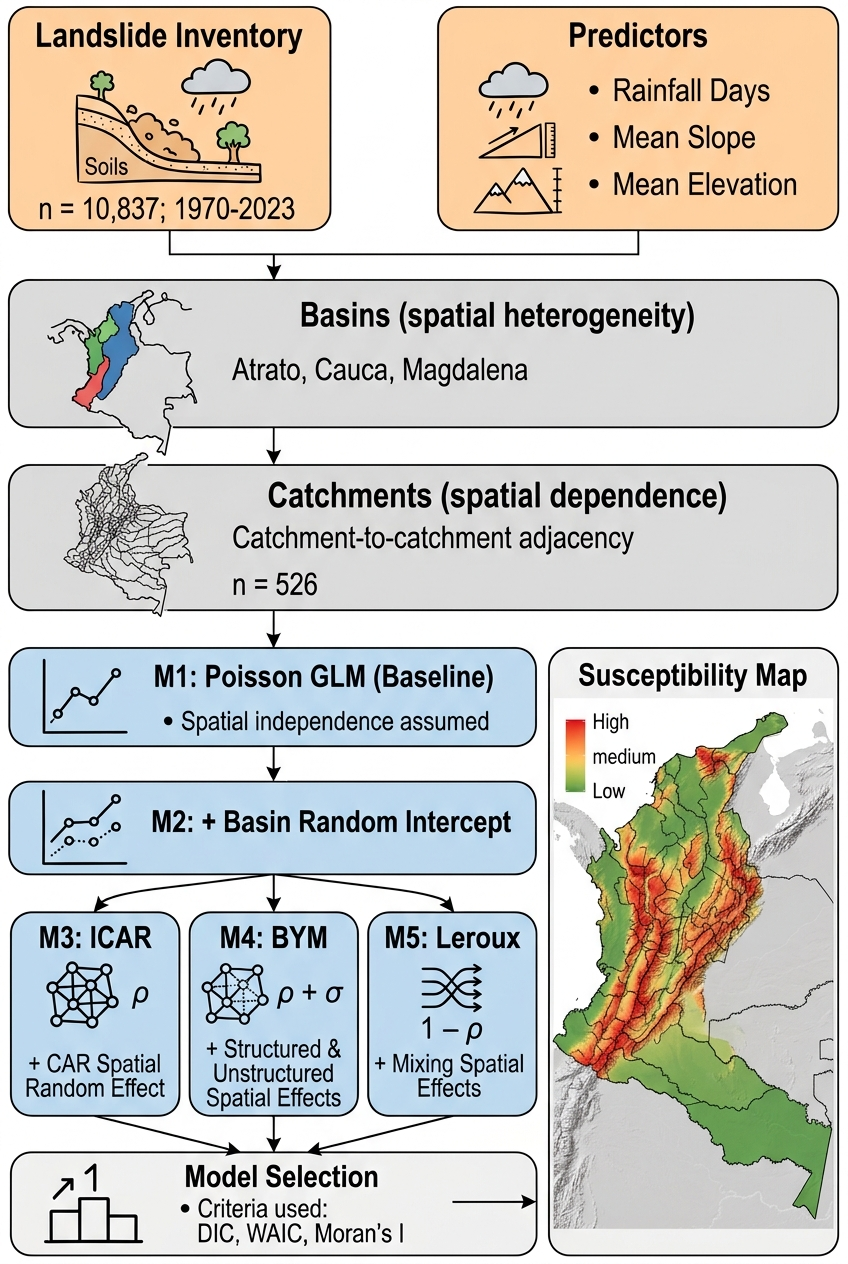
\includegraphics[width=0.65\textwidth,height=0.85\textheight,keepaspectratio]{Fig01_workflow.jpg}
\caption{\hlG{Modeling workflow, from data inputs through the progression of models (M1-M5) to model diagnostics, model selection, and the resulting susceptibility map.}}
\label{FigWorkflow}
\end{figure}

\hl{The three primary drainage basins (Atrato, Cauca, and Magdalena) constitute the upper level (Fig. 2). 
These basins broadly coincide with distinct structural and lithological domains of the northern Colombian Andes: the Pacific-facing Western Cordillera and Choc\'{o} block drained by the Atrato, the inter-Andean Cauca depression flanked by volcanic and metamorphic terranes, and the Magdalena valley between the Central and Eastern Cordilleras }\citep{Cediel2003, Taboada2000}\hl{, which motivates their use as the upper-level grouping for regional heterogeneity, independently of the spatial random-effects model. 
The 526 smaller catchments nested within these basins constitute the lower-level Terrain Mapping Units (TMUs), the scale} \hlE{at which we analyse the spatial clustering of landslide activity;} \hl{we represent this local dependence using several conditional autoregressive structures, described below.}

\hl{We adopt catchments, rather than slope units or pixels, as the terrain mapping unit because our response variable is a landslide count per unit, not a binary presence/absence outcome. 
A Poisson count formulation is designed for data aggregated over areal units and does not require the slope-scale resolution that a presence/absence classification would }\citep{lombardo2020space}\hl{. 
Regional- and national-scale susceptibility assessments necessarily operate at resolutions coarser than the individual slope, and catchment- or basin-scale predictors are an established way to represent bulk terrain conditions at such scales }\citep{guzzetti2005probabilistic, stanley2017heuristic, nowickijessee2018global}\hlE{. 
Accordingly, mean catchment slope and elevation are treated here as descriptors of each catchment as a whole, not as proxies for the local conditions under which individual slopes fail. Mean catchment slope expresses the bulk steepness of a catchment, which reflects landscape state, incision and relief and scales with landslide erosion at the catchment scale }\citep{Montgomery2002, Larsen2012}\hlE{; it is not a proxy for the critical slope angle at which landslides initiate, and its coefficient is a between-catchment association. We verified that aggregating slope to catchment means does not mask the slope-scale control on landslide occurrence in the modelled counts: a slope-scale response estimated from within-catchment contrasts alone, integrated over every 12.5~m cell of each catchment, yields a covariate almost collinear with mean slope ($r = 0.98$) and leaves the fitted models and their latent spatial structure essentially unchanged (\mbox{Appendix~\ref{secA6}}).}

The study area in the northern Colombian Andes is a tectonically active, mountainous region characterized by steep topography, deep weathering profiles, and intense seasonal rainfall. 
Consequently, the landscape is dominated by frequent, rainfall-induced slope failures. 
Our landslide inventory is predominantly composed of shallow translational soil slides and debris flows, which typically mobilize residual soils and saprolite on hillslopes steeper than 25$^{\circ}$. 
We compiled this inventory of 10,837 that occurred between 1970 and 2023 (Fig. 2) from manual mapping based on true-color optical images from Google Earth Pro (provided by Maxar/Airbus Technologies and Landsat/Copernicus), at a nominal resolution of $<$1 m. 
\hlG{Each landslide is represented in the inventory as a single point at its approximate crown location.}

\begin{figure*}[t]
\centering
\begin{tabular}{@{}l@{\hspace{4mm}}l@{}}
\textbf{A} & \textbf{B} \\
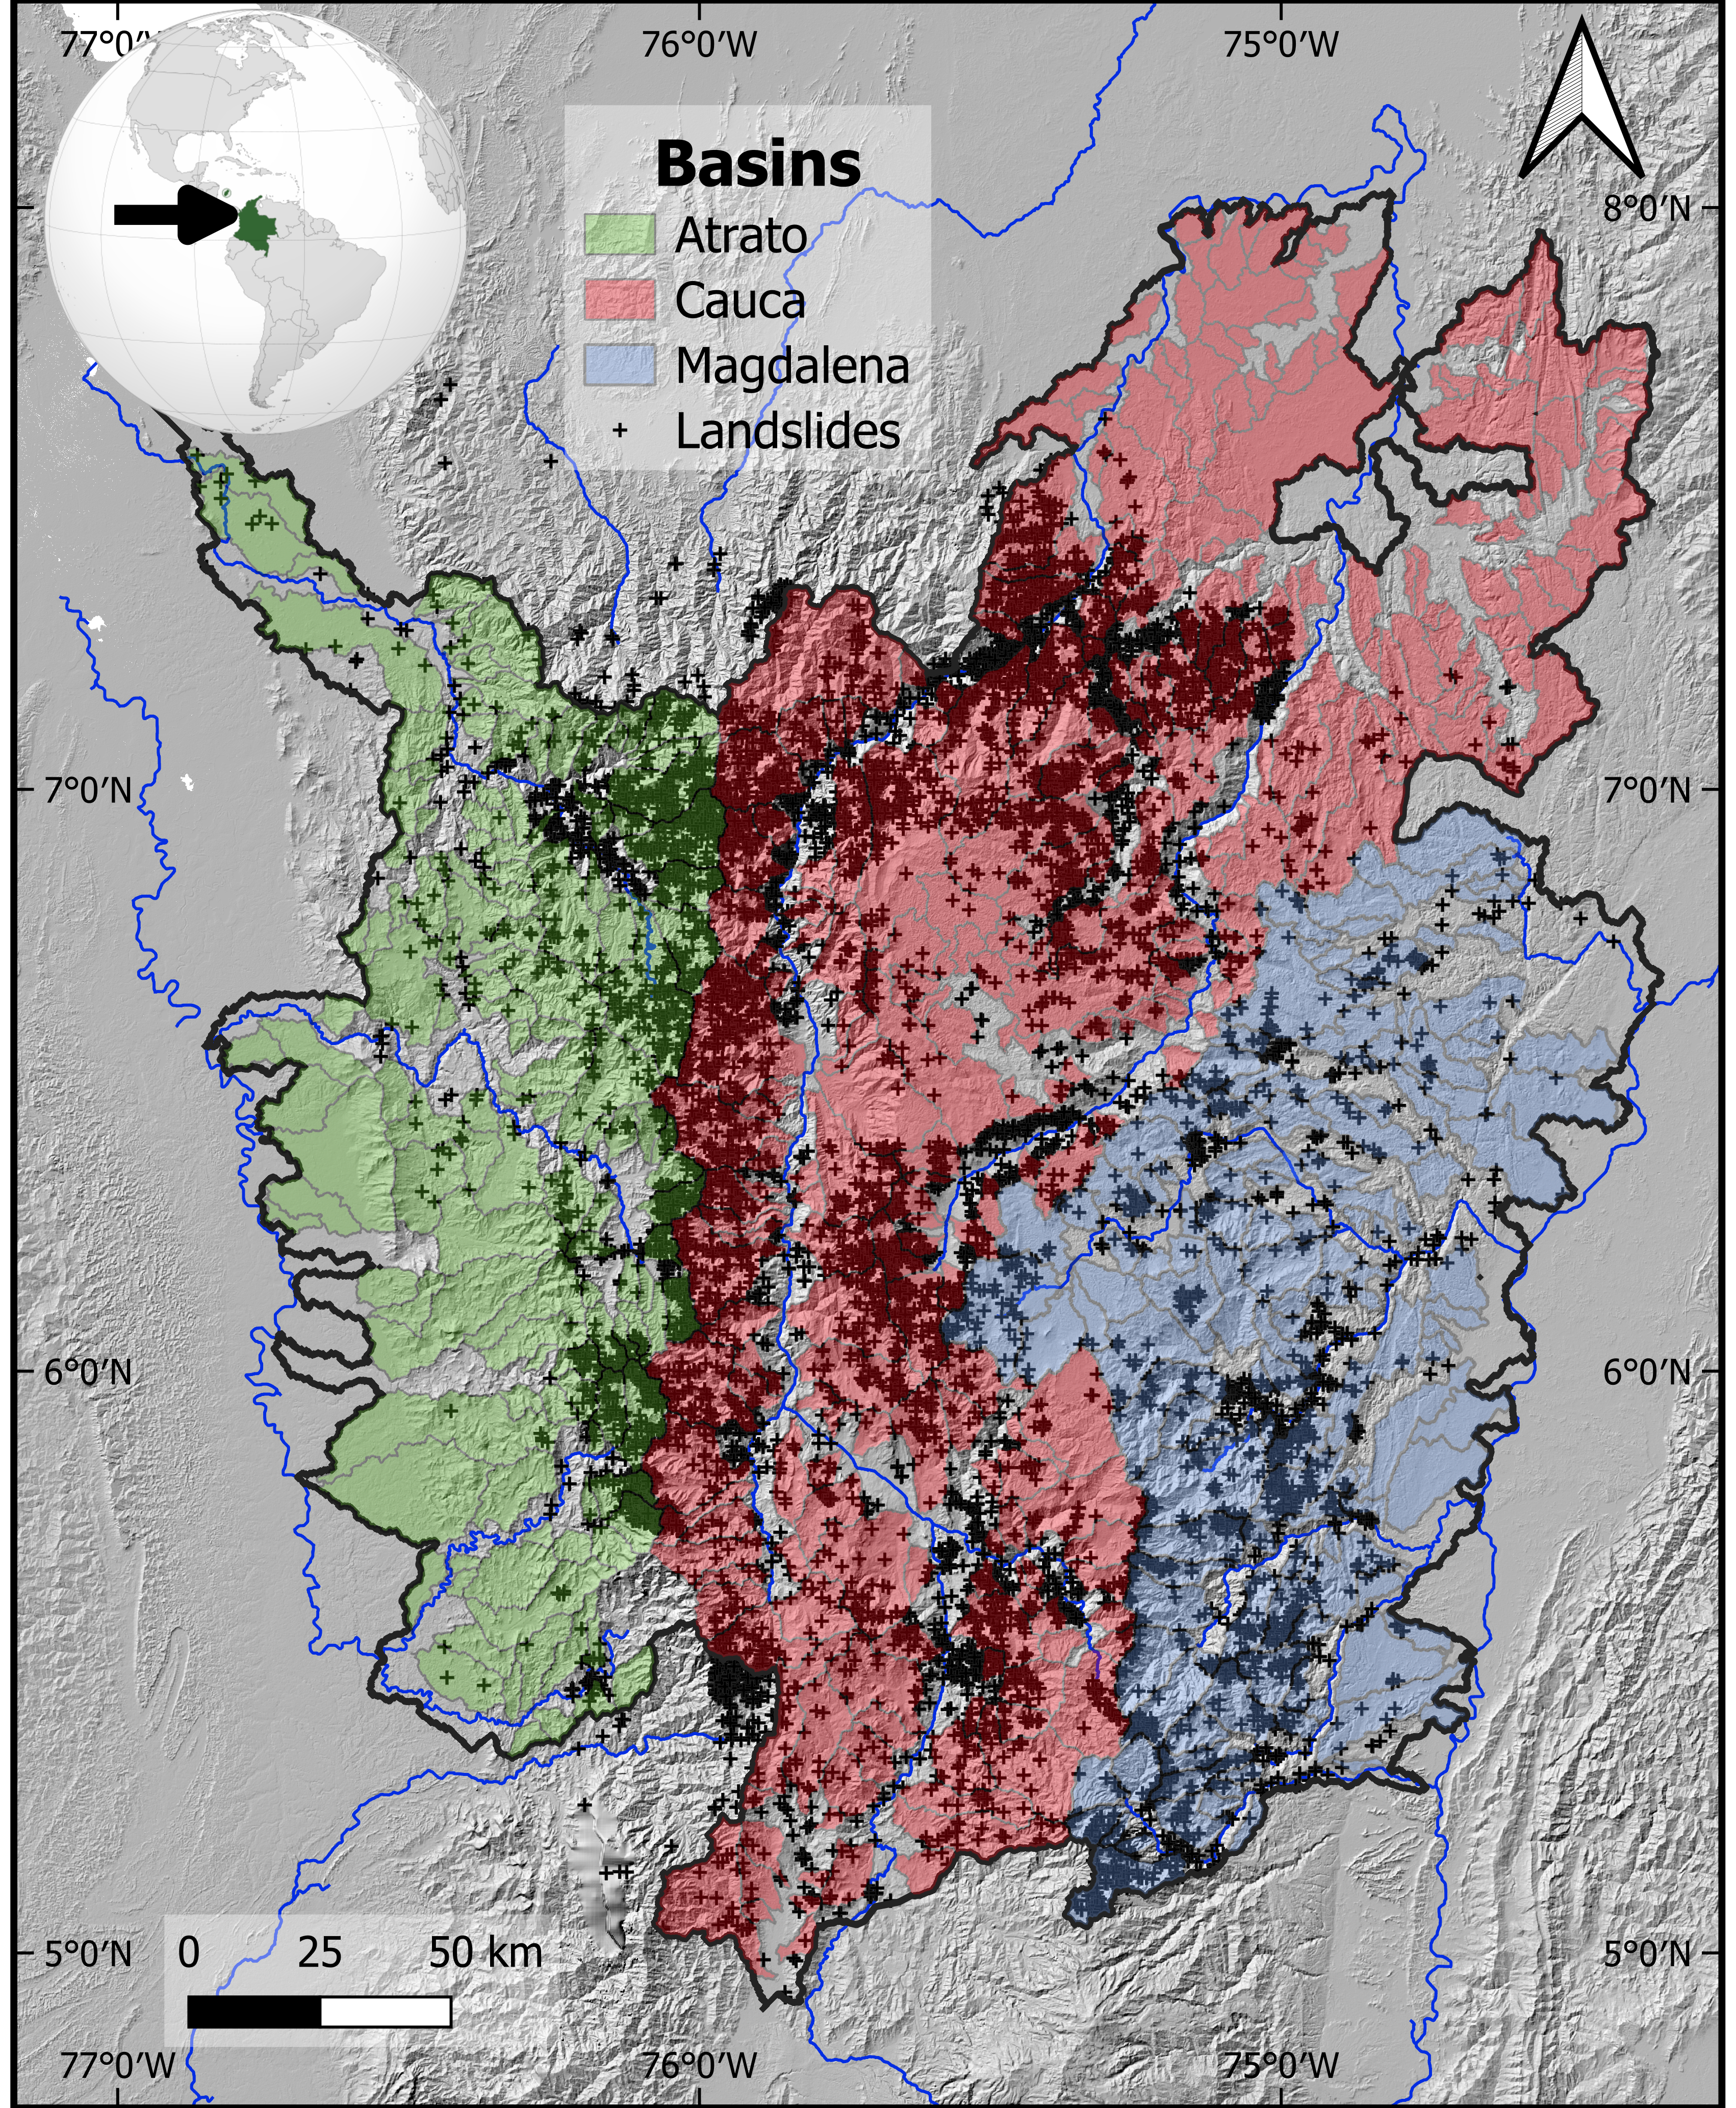
\includegraphics[height=0.6\textwidth]{Fig02a_study_area.png} & 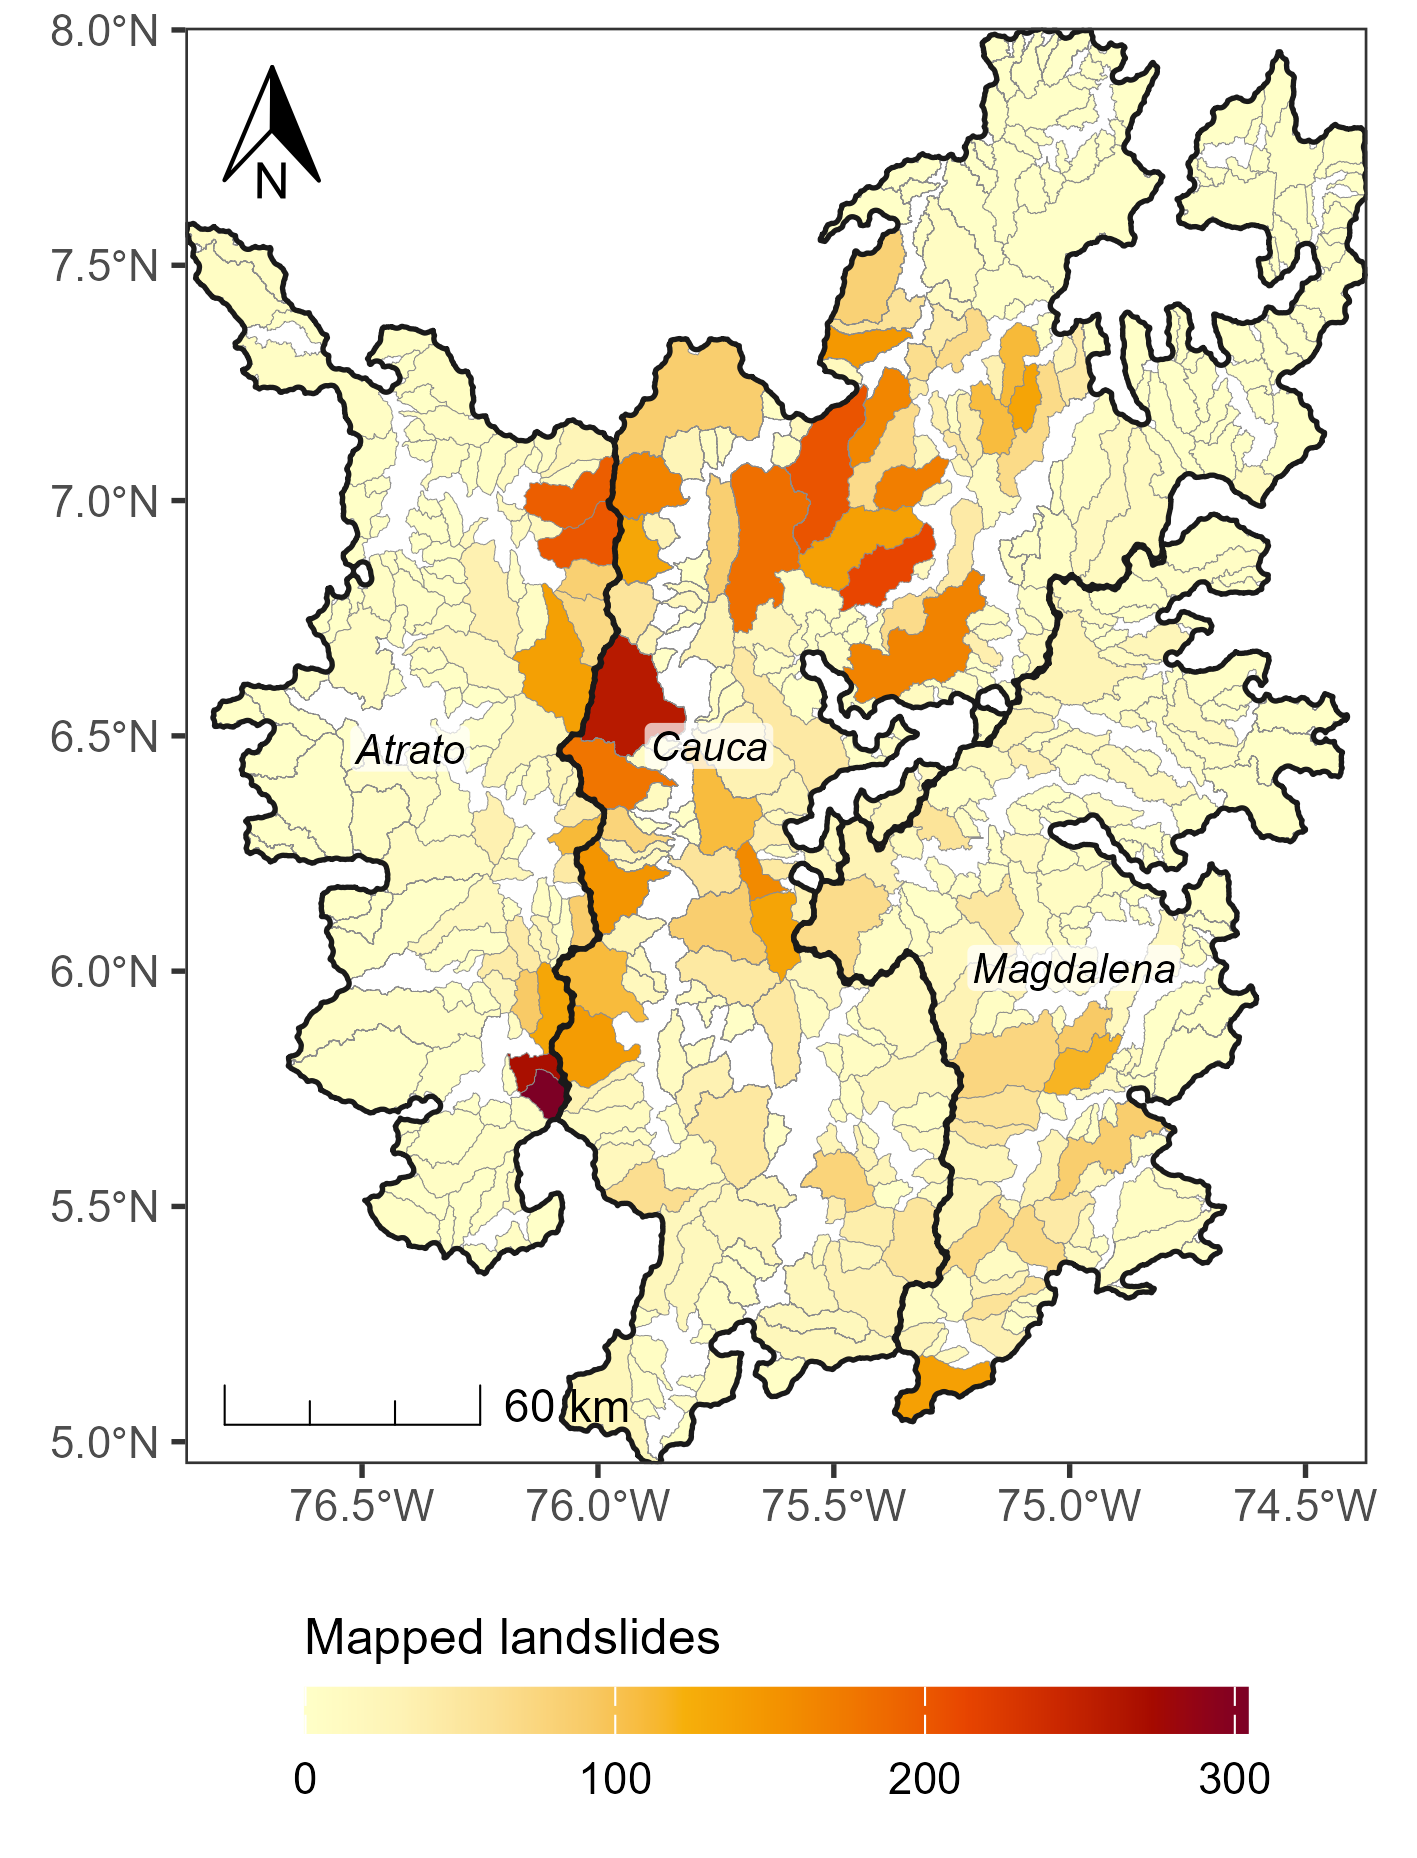
\includegraphics[height=0.6\textwidth]{Fig02b_landslide_counts.png}
\end{tabular}
\caption{Landslide occurrences. (A) Study area in the northern Colombian Andes with the three main basins \hlE{and the 10,837 landslides} mapped using Google Earth Pro (Imagery © 1970-2023 Google, Maxar/Airbus Technologies \& Landsat/Copernicus). \hlE{(B) Number of mapped landslides per catchment.}}
\label{Fig2}
\end{figure*}

We derived the terrain parameters from the digital elevation model (DEM) of the Advanced Land Observing Satellite-Phased Array-Type L-Band Synthetic Aperture Radar (ALOS-PALSAR) at a resolution of 12.5 m \citep{logan2014radiometrically}. 
We computed rainfall from 1981 to 2023 with Google Earth Engine (GEE) using the Climate Hazard Group InfraRed Precipitation with Station Data (CHIRPS) \citep{funk2015climate} version 2.0 at a 5-km resolution.

\hl{To select predictors, we first screened a broad candidate set using Pearson correlation and Principal Component Analysis (PCA) }\citep{reichenbach2018review}\hl{: the number of days with rainfall totals $>$20 mm ($R_d$), mean elevation ($H$), mean slope ($S$), catchment area, hypsometric integral, lineament density, mean relief, mean annual rainfall, the topographic wetness index (TWI), a curvature index, and stream drainage density, together with two categorical layers, land cover and lithology.}

\hl{Mean annual rainfall ($r = 0.98$ with $R_d$), lineament density ($r = 0.91$ with $S$), mean relief ($r = 0.96$ with $S$), and TWI ($r = -0.80$ with $S$) all exceeded the $|r| > 0.75$ multicollinearity threshold against a candidate retained predictor and were excluded. 
Catchment area, hypsometric integral, curvature, and drainage density fell below this threshold but showed weak association with $R_d$, $H$, and $S$ alike ($|r| < 0.4$ in every case); curvature and drainage density in particular lose most of their spatial signal once averaged over catchment-sized units, and were not retained as separate predictors. 
Land cover and lithology are available in the catchment dataset only as coarse, catchment-majority categorical classes (two land-cover classes and three lithological classes, respectively) and were not included as continuous fixed effects for this reason; mean elevation partially proxies for both, and finer-resolution categorical layers are a priority for future refinement of this framework.}

\hl{This screening retained three predictors: $R_d$, $H$, and} \hlE{$S$; the full correlation matrix is given in \mbox{Appendix~\ref{secA2}} (\mbox{Table~\ref{tabA2}}).} 
\hl{These were selected for their direct physical relevance to landslide initiation. 
$S$} \hlE{describes the bulk steepness of a catchment, which, through its relation to hillslope gradient, relief and incision, is expected to scale with the landslide activity of the catchment.} 
\hl{$R_d$ acts as a proxy for the frequency of triggering events; intense rainfall increases pore-water pressure within the soil. 
Finally, $H$ often serves as an effective proxy for a combination of factors, including orographic effects on precipitation, variations in geological materials and weathering, and changes in land cover, all of which strongly influence slope stability.}

The spatial structure at the lower level was represented employing the Queen adjacency rule \citep{moraga2023spatial}, where TMUs are considered neighbors if they share at least one border. 
The derived spatial contiguity weight and covariance matrices are shown in Figure 3.

\begin{figure}[h]
\centering
\begin{tabular}{@{}l@{\hspace{4mm}}l@{}}
\textbf{A} & \textbf{B} \\
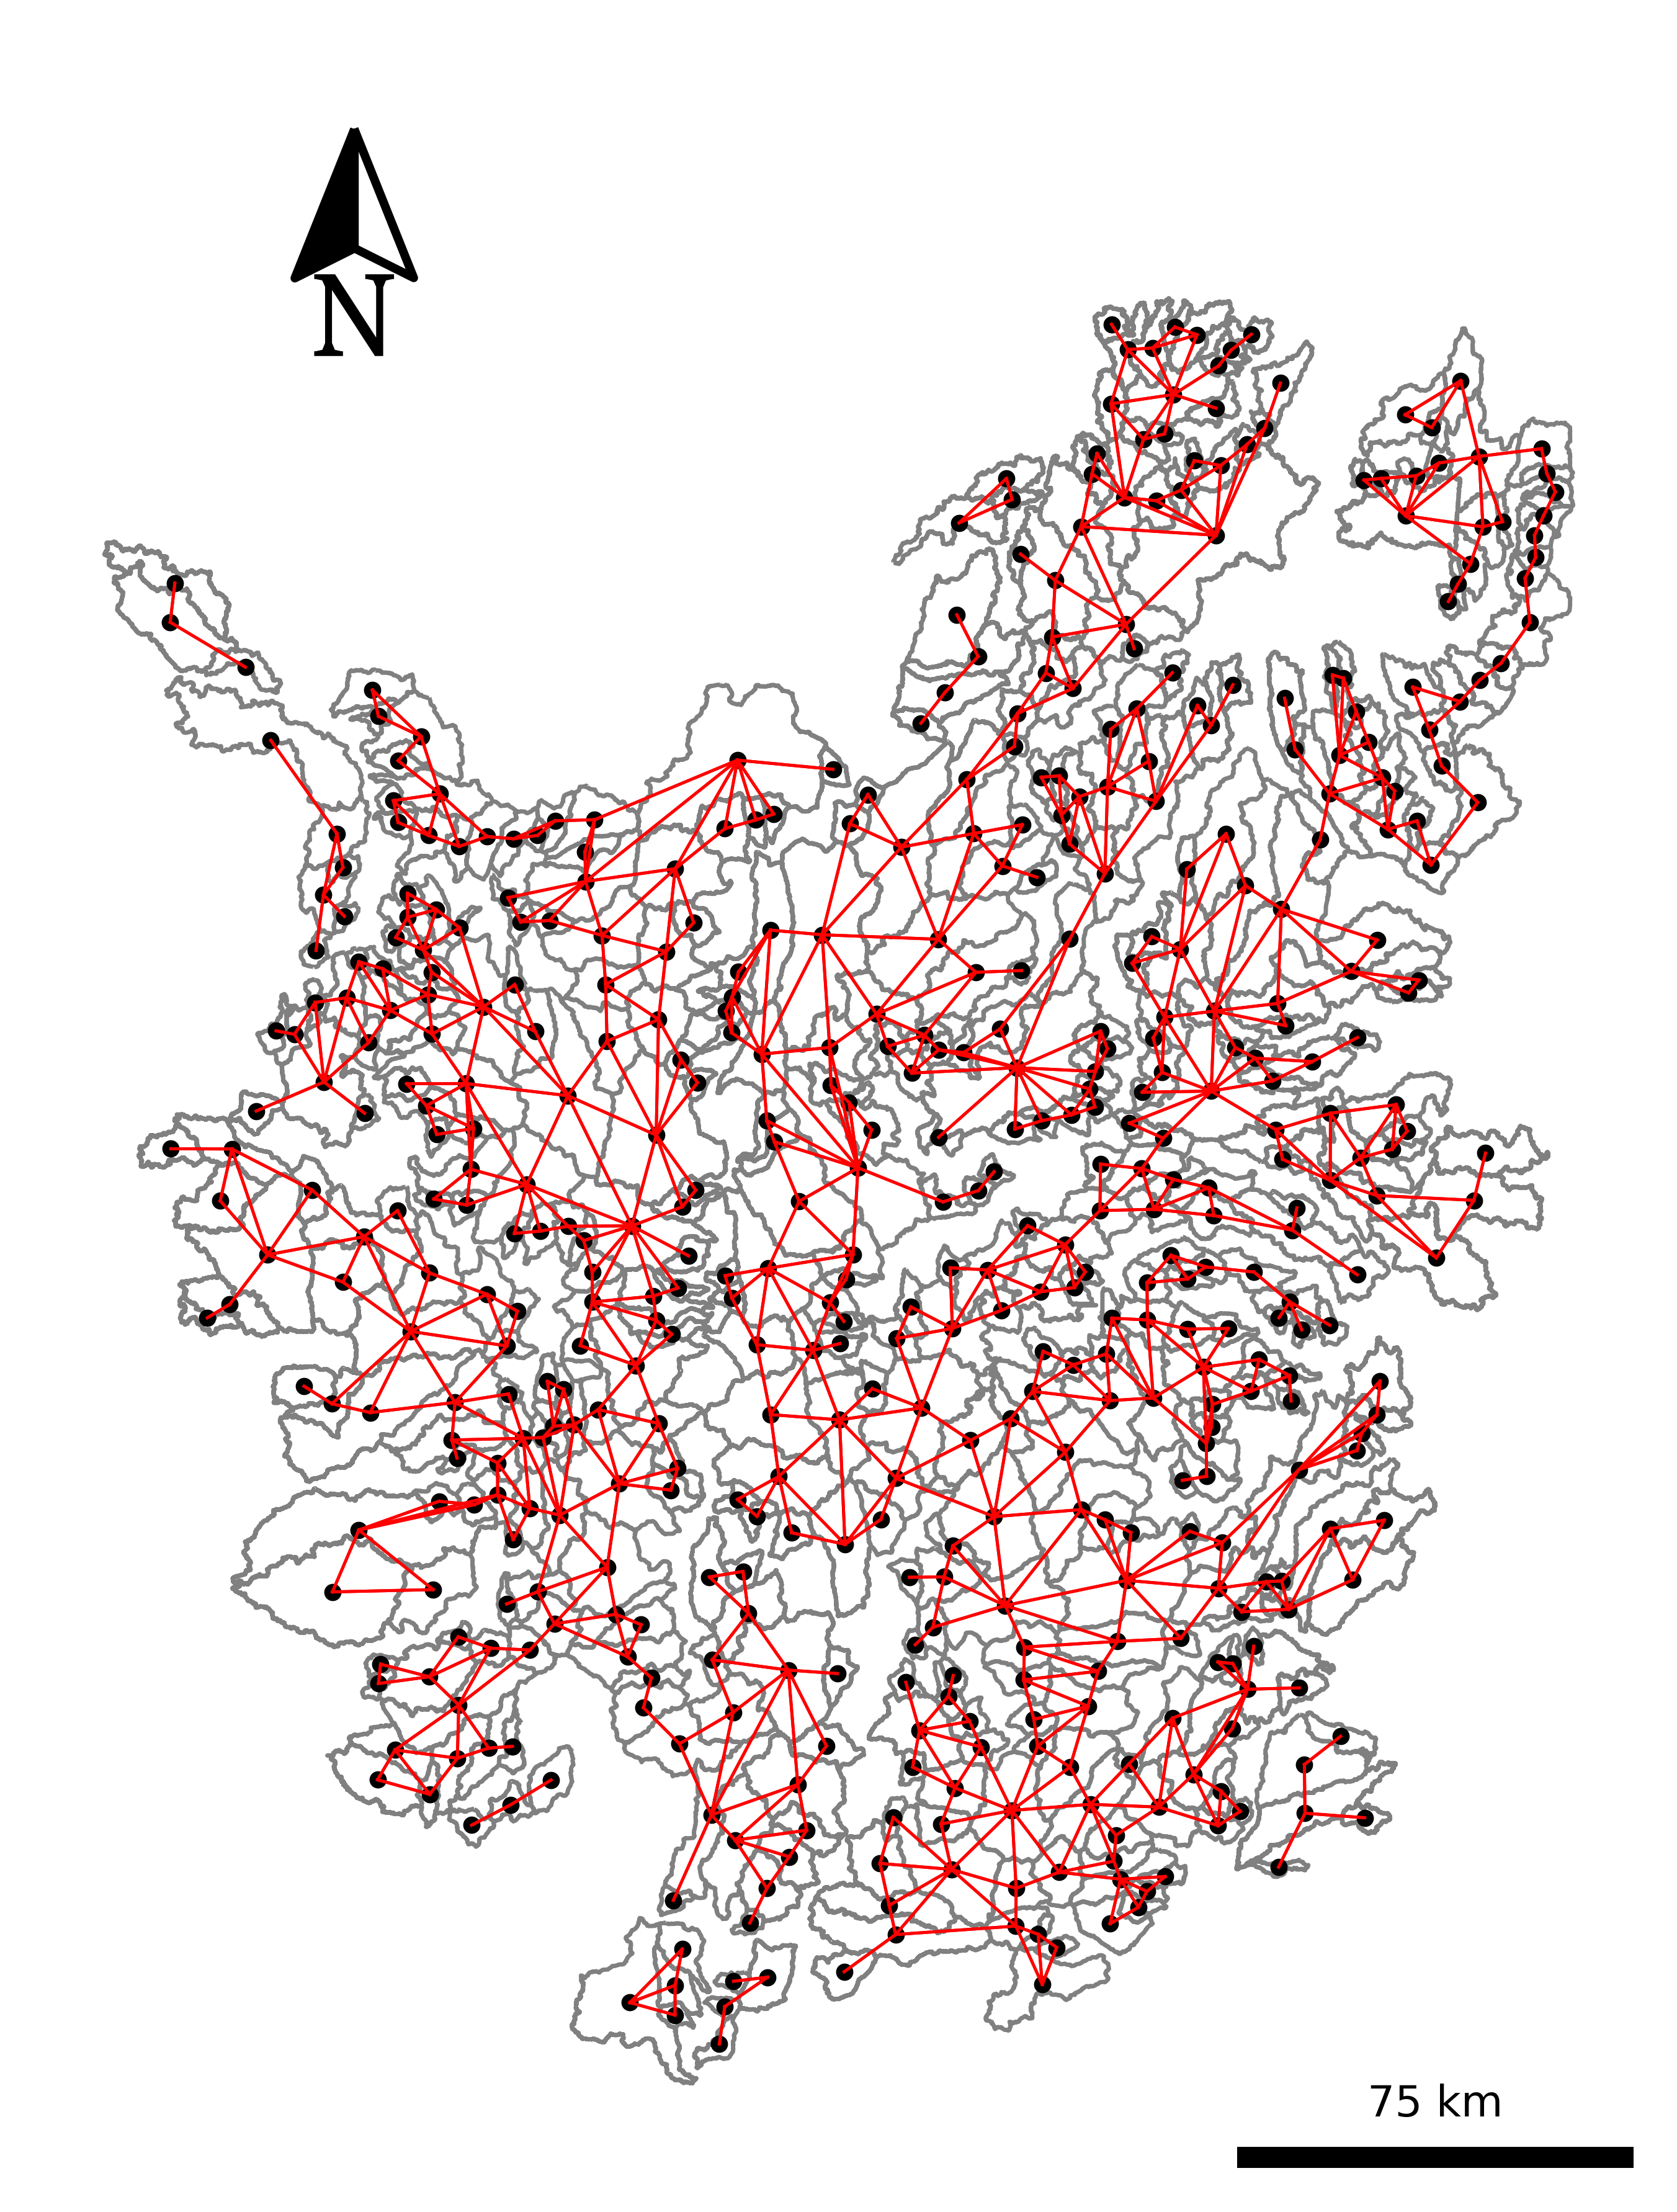
\includegraphics[height=0.6\textwidth]{Fig03a_neighbour_graph.png} & 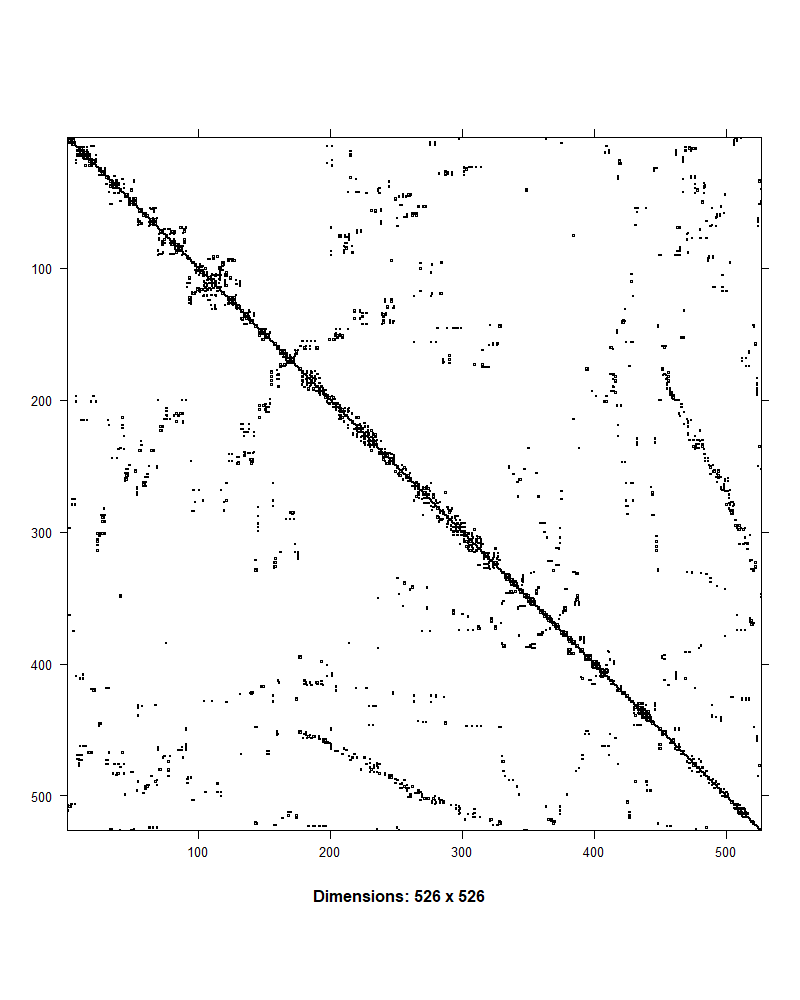
\includegraphics[height=0.6\textwidth]{Fig03b_adjacency_matrix.png}
\end{tabular}
\caption{Spatial contiguity (Queen) structure of the 526 catchments. \hlE{(A) Neighbour graph linking the centroids of adjacent catchments. (B) The corresponding $526 \times 526$ binary adjacency matrix.}}
\label{Fig3}
\end{figure}

\hl{To diagnose residual spatial autocorrelation for each fitted model, we compute Moran's I statistic }\citep{anselin2019moran}\hl{ on the standardized Pearson residuals $e_i$:}

\begin{equation}\label{eq:moran}
I = \frac{n}{S_0} \frac{\sum_{i=1}^n \sum_{j=1}^n w_{ij}(e_i - \bar{e})(e_j - \bar{e})}{\sum_{i=1}^n (e_i - \bar{e})^2}
\end{equation}

\hl{where $n$ is the number of catchments, $w_{ij}$ is the} \hlE{row-standardized} \hl{Queen adjacency weight between catchments $i$ and $j$ defined above, and $S_0 = \sum_{i=1}^n \sum_{j=1}^n w_{ij}$. 
Values of $I$ close to $+1$ indicate strong positive residual spatial autocorrelation (neighboring catchments with similar residuals), values close to $-1$ indicate a checkerboard (locally over-dispersed) pattern, and values near 0 indicate spatially random residuals. 
We assess the statistical significance of $I$ via a Monte Carlo permutation test with 999 permutations.}

\hl{The specifications of the five models compared in this study, shown in the workflow of Fig. 1, are given below.}

\hl{\textbf{M1 -- Simple Poisson model.} Our simplest model (M1) is a standard Poisson GLM in which the expected landslide count, $\lambda_i$, is modeled as a function of three predictors. The linear predictor is defined as:}

\begin{equation}
\eta_i = \beta_0 + \beta_1 Rd_i + \beta_2 S_i + \beta_3 H_i + \log(A_i)
\end{equation}

\hl{where $Y_i$ is the number of landslides in catchment $i$, modeled as a function of the number of days with rainfall exceeding 20 mm ($Rd$), mean catchment slope ($S$), and mean catchment elevation ($H$), with an offset term, $\log(A_i)$, normalizing for catchment area ($A_i$).}

\hl{\textbf{M2 -- Random intercept model at basin level.} This model extends M1 with an unstructured latent random effect at the basin level (Cauca, Magdalena, and Atrato):}

\begin{equation}
Y_{ij} \sim Poisson(\lambda_{ij}), \lambda_{ij} = \exp(\beta_0 + \beta_1 Rd_{i} + \beta_2 S_i + \beta_3 H_i + u_j + \log(A_i))
\end{equation}

\hl{where $u_j$ is the random intercept for basin $j$, capturing unobserved heterogeneity among the known basins.}

\hl{\textbf{M3 -- ICAR model.} This model retains the basin-level random intercept from M2 and additionally accounts for local spatial dependency at the TMU level via the Intrinsic Conditional Autoregressive (ICAR) structure:}

\begin{equation}
Y_i \sim Poisson(\lambda_i), \lambda_i = \exp(\beta_0 + \beta_1 Rd_i + \beta_2 S_i + \beta_3 H_i + v_{j[i]} + u_i)
\end{equation}

\hl{where $v_{j[i]}$ is the basin-level random intercept for the basin containing catchment $i$, as in M2, and $u_i$ is a catchment-level spatial random effect that follows an ICAR structure. The ICAR prior for $u_i$ is defined as:}

\begin{equation}
u_i | \{u_j : j \neq i\} \sim N \left( \frac{1}{n_i} \sum_{j \in N(i)} u_j, \frac{\sigma^2}{n_i} \right)
\end{equation}

\hl{which ensures that spatially neighboring units have similar random effects, imposing smoothness on the spatial structure.}

\hl{\textbf{M4 -- Besag--York--Molli\'{e} (BYM) model.} This model also retains the basin-level random intercept from M2, and replaces the catchment-level ICAR term with the BYM specification, which combines a spatially structured and an unstructured random effect at the catchment level:}

\begin{equation}
Y_i \sim Poisson(\lambda_i), \lambda_i = \exp(\beta_0 + \beta_1 Rd_i + \beta_2 S_i + \beta_3 H_i + v_{j[i]} + u_i)
\end{equation}

\hl{where $v_{j[i]}$ is the basin-level random intercept, as in M2 and M3, and $u_i$ denotes the combined structured-plus-unstructured catchment-level term, jointly accounting for local spatial dependence and unstructured overdispersion.}

\hl{\textbf{M5 -- Leroux model.} Lastly, this model again retains the basin-level random intercept from M2, and replaces the catchment-level term with the Leroux specification, which introduces a single mixing parameter to control the degree of spatial smoothing:}

\begin{equation}
Y_i \sim Poisson(\lambda_i), \lambda_i = \exp(\beta_0 + \beta_1 Rd_i + \beta_2 S_i + \beta_3 H_i + v_{j[i]} + u_i)
\end{equation}

\hl{where $v_{j[i]}$ is the basin-level random intercept, as in M2-M4, and $u_i$ follows a Leroux prior:}

\begin{equation}
u_i \sim N \left( \rho \sum_{j \in N(i)} w_{ij} u_j, (1 - \rho) \sigma^2 \right)
\end{equation}

\hl{with $\rho$ controlling the balance between spatial dependence and independence, allowing flexibility in the spatial structure.}

%%%%%%%%%%%%%%%%%%%%%%%%%%%%%%%%%%%%%%%%%%%%%%%%%%%%%%%%%%%%%%%%%%%%%%%%%%%%%%%%

\section{Results}\label{sec4}

We present the results from a series of five hierarchical models designed to assess landslide susceptibility in the northern Colombian Andes. 
This series follows a progression of increasing complexity to systematically evaluate the impact of spatial effects. 
We begin with a simple Poisson model (M1) to estimate the predictor effects on landslide counts, assuming spatial independence. 
We then introduce a multilevel model (M2) that incorporates random intercepts at the upper level (basins). 
We further extend this structure by modeling spatial dependence at the lower level (catchments) with Conditional Autoregressive (CAR) structures in the random effects. 
We explore three increasingly flexible spatial models: the Intrinsic Conditional Autoregressive (ICAR) model (M3), the Besag--York--Molli\'{e} (BYM) model (M4), and the Leroux model (M5). 
This progression of models, from a simple non-spatial baseline to different spatial formulations, enhances the capacity to represent both large-scale spatial heterogeneity and local spatial dependency, providing a more comprehensive framework for capturing the spatial complexity of landslide processes.

\subsection{Model 1: Simple Poisson model}\label{subsec41}

\hl{This simple Poisson model reveals significant positive relationships between landslide occurrence and all predictors. 
As in M2-M5, all predictors were standardized (mean 0, SD 1) prior to fitting; the coefficients in Table 1 and the Rate Ratios (RR) below are therefore expressed per one standard deviation (SD) increase in each predictor, not per raw unit. 
(e.g., for a 1-SD increase in mean catchment slope ($\mathrm{SD} = 6.8^{\circ}$), the expected count multiplies by 1.85 (RR = 1.85, 95\% CrI excludes zero)).
Expressed instead in physically interpretable raw units, these correspond to a 9.5\% increase in expected landslide count per additional degree of mean slope, a 5.6\% increase per 100 m of mean elevation, and a 1.4\% increase per 100 additional rainfall days. 
These results highlight mean slope as the predictor with the strongest standardized effect on landslide rates.}

The Moran’s statistic indicates residual spatial autocorrelation, which may reduce the reliability of the model estimates, and suggests the need for additional spatial effects or a more sophisticated spatial structure. 
This strong spatial clustering in the residuals (Fig. 4) is a clear statistical signal of unmodeled physical processes. 
It indicates that our predictors (slope, rain, elevation) are insufficient on their own to explain where landslides are concentrated, \hl{consistent with an unmeasured, spatially structured factor not captured by the current predictor set.}

\hl{Beyond spatial autocorrelation, the standardized Pearson residuals for M1 also reach magnitudes of} \hlE{up to 35} \hl{in a subset of catchments (Fig. 4B), well outside the range expected under a correctly specified Poisson model. 
This indicates pronounced overdispersion, i.e. the variance of landslide counts substantially exceeds the Poisson assumption of equal mean and variance.} 
\hlE{The counts are strongly overdispersed: across the 526 catchments their variance is 1690 against a mean of 20.6 (a variance-to-mean ratio of 82), and 144 catchments (27\%) contain no mapped landslide, whereas a Poisson distribution with the observed mean would produce essentially none. Posterior predictive checks confirm that M1 fails to reproduce both features, predicting 21 zero-count catchments (95\% interval 14--29) and a count variance of 918 (850--992) (\mbox{Appendix~\ref{secA5}}).} \hl{Overdispersion of this magnitude can arise from several non-exclusive sources, including unmodeled spatial dependence, missing covariates, and the change-of-support entailed by aggregating} \hlE{landslides to catchments. Replacing the Poisson by a negative-binomial likelihood lowers the DIC of M1 from 10,941 to 3,453; how the spatial models treat this extra-Poisson variability is examined in \mbox{Sect.~\ref{subsec51}}.}

\hl{We also tested whether the assumption of a linear relationship between each standardized predictor and the log-expected landslide count is adequate. 
Adding a quadratic term to the M1 specification improved the fit substantially for mean elevation ($\Delta$AIC = 462) and mean slope ($\Delta$AIC = 227; both likelihood-ratio $p < 10^{-50}$), but not for rainfall days ($p = 0.48$). 
A penalized spline for slope improved the fit further ($\Delta$AIC = 480 relative to the linear model). 
The fitted quadratic term for slope is concave (coefficient $= -0.196$, $p < 10^{-45}$), indicating a diminishing marginal effect of slope at the highest values observed, consistent with a physical ceiling on shear-stress-driven susceptibility, though the small number of catchments at the highest slopes limits how precisely this saturation can be} \hlE{characterized (\mbox{Fig.~\ref{figA2}}).} 
\hl{Because this simplification applies identically across M1--M5, it does not confound our comparison of spatial versus non-spatial random-effects structures, but it does mean that the fixed-effect estimates in Table 1 should be interpreted as linear approximations to a more complex underlying relationship.}

\begin{figure}[h]
\centering
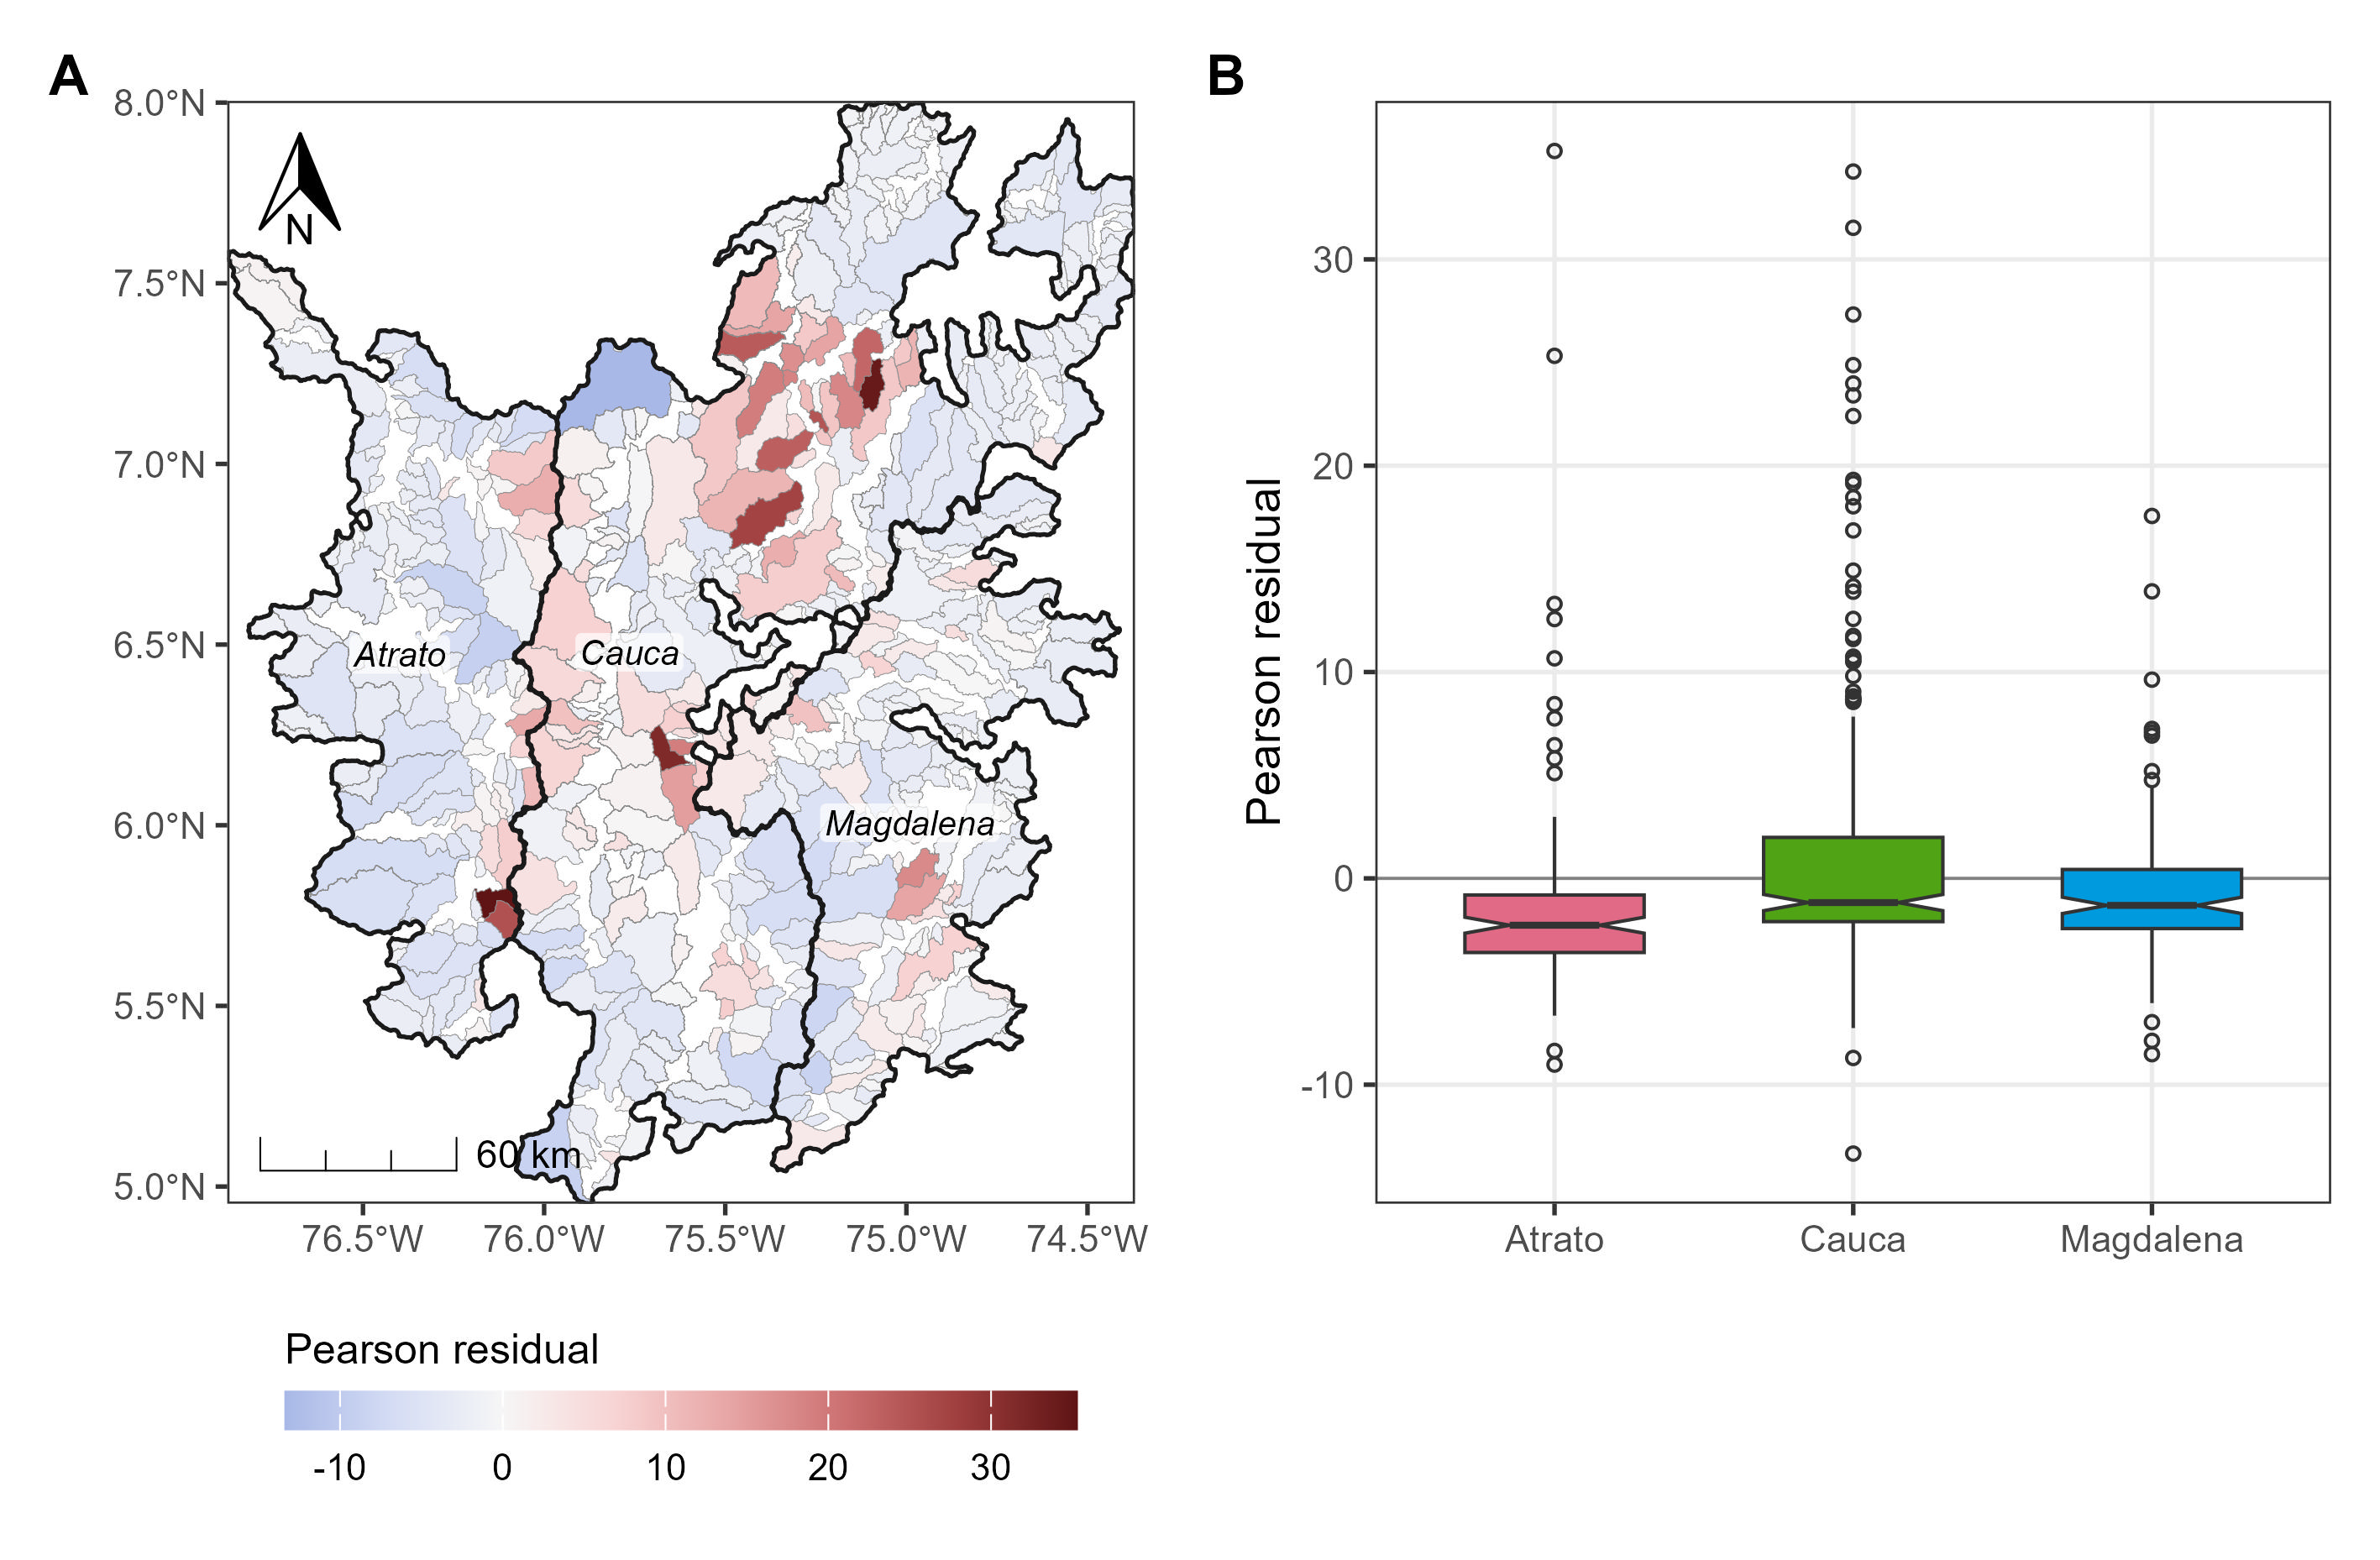
\includegraphics[width=0.8\textwidth]{Fig04_M1_poisson.jpg}
\caption{Model M1 – Standard Poisson. \hlE{(A) Pearson residuals from the baseline Poisson model without spatial effects (M1). (B) Distribution of the residuals by basin.} The residuals show pronounced spatial clustering, indicating strong residual spatial autocorrelation. The high Moran’s Index (MI = 0.513) supports the presence of unaccounted spatial structure in the model.}
\label{Fig4}
\end{figure}


\subsection{Model 2: Random intercept model at basin level}\label{subsec42}

Prior to modeling, all predictors were standardized (e.g., scaled to a mean of 0 and a standard deviation of 1). 
After fitting the model, all three predictors showed credible positive effects. 
In particular, slope and elevation show relatively high posterior means (0.661 and 0.485, respectively), suggesting strong contributions to landslide susceptibility. 
While the effect of rainfall days is small (0.299), it remains positive.

The global intercept of the model represents the average baseline landslide susceptibility for the entire study area (i.e., the mean across all 526 catchments). 
The basin-specific random effects are then interpreted as deviations from this overall average. 
Among these effects, only the Cauca basin has a positive posterior mean (0.311), indicating a higher baseline susceptibility relative to this global intercept. 
Conversely, the Atrato and Magdalena basins show negative or near-zero values, suggesting either inherently lower landslide activity or that their local variability is better captured by other, likely catchment-level predictors.

\hl{This M2 formulation (DIC = 9,469; WAIC = 20,795) shows a notable improvement in model fit over the non-spatial M1 benchmark (DIC = 10,941; WAIC = 27,104).} 
Furthermore, the residual Moran’s Index (MI) decreases substantially from 0.513 (M1) to 0.447 (M2), indicating that incorporating basin-level heterogeneity successfully reduced some of the residual spatial autocorrelation. 
This reduction shows that some of the spatial clustering is due to large-scale regional differences between basins (e.g., the Cauca basin being inherently more susceptible). 
However, the still-high Moran’s I confirms that most of the spatial structure exists at a local, catchment-to-catchment scale.

\begin{figure}[h]
\centering
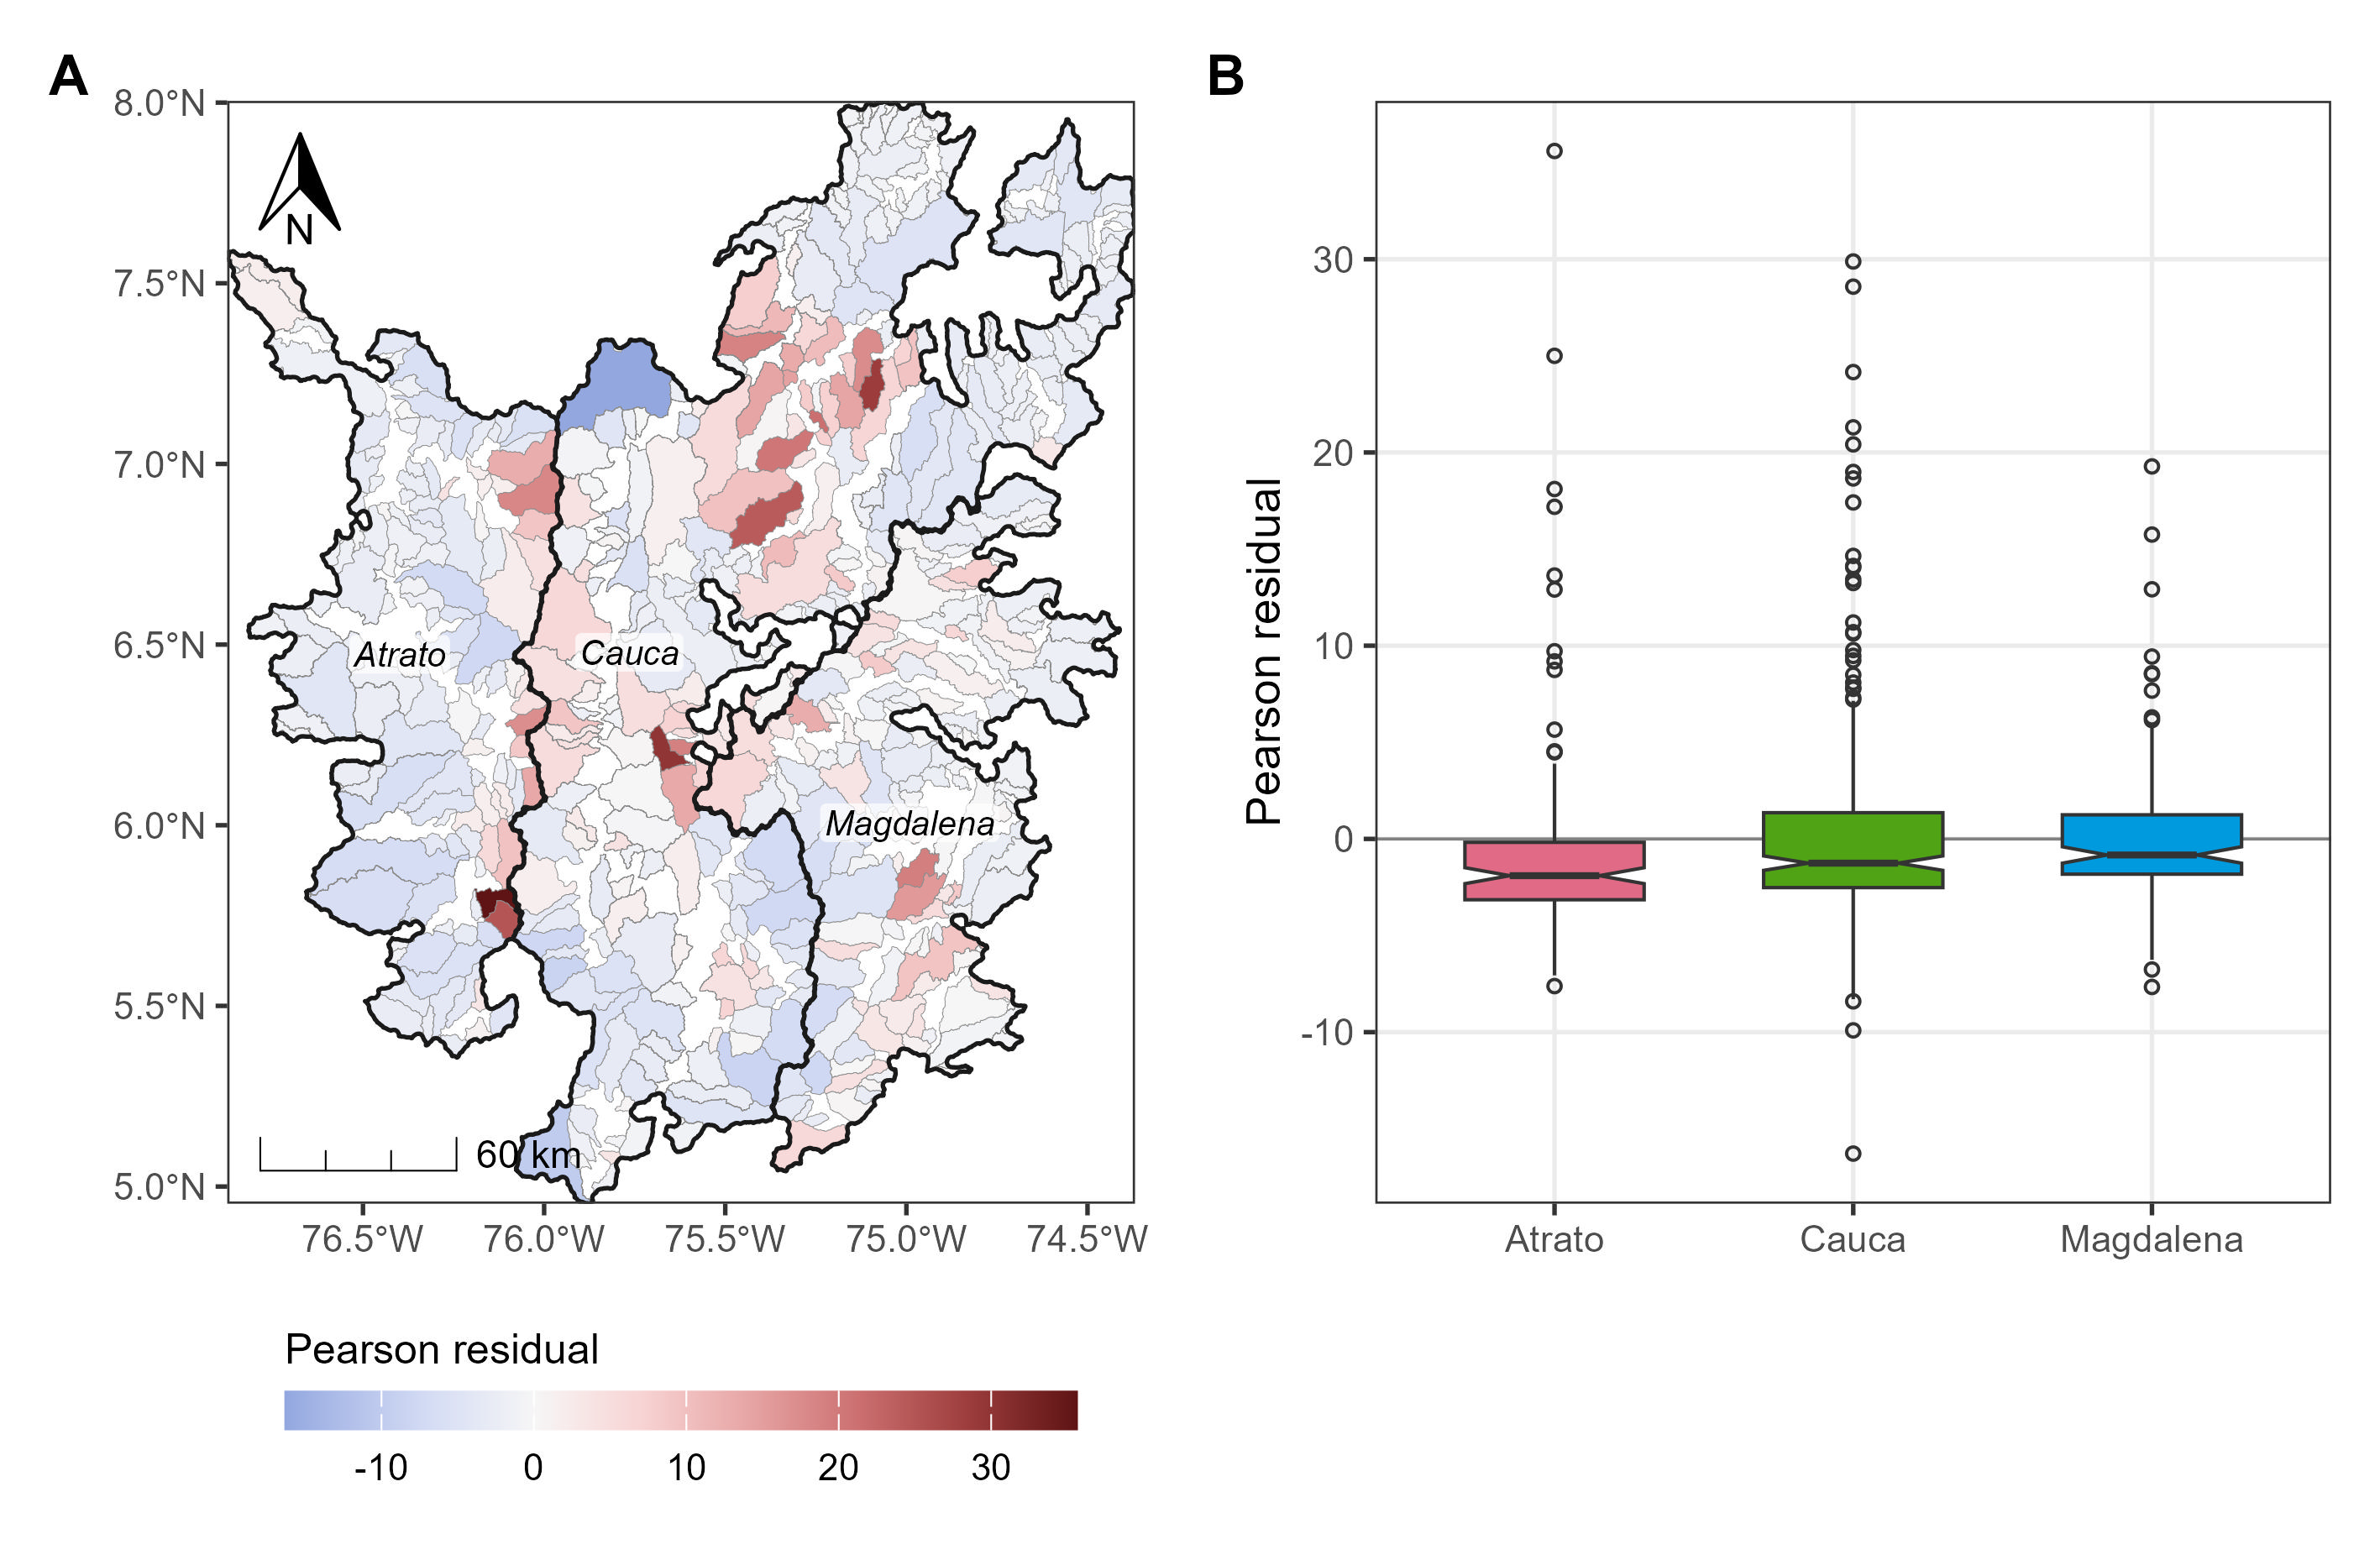
\includegraphics[width=0.8\textwidth]{Fig05_M2_basin_intercepts.jpg}
\caption{Model M2 – Multilevel Poisson with Random Effects at Basin Level. (A) Pearson residuals from the multilevel Poisson model including an unstructured random intercept at the basin level (Atrato, Cauca, Magdalena). (B) Distribution of residuals by basin. While the inclusion of upper-level heterogeneity reduces some regional variability, spatial clustering of residuals remains apparent—especially in the Cauca basin—suggesting unaccounted local spatial dependence. The residual Moran’s Index (MI = 0.447) confirms the persistence of moderate spatial autocorrelation, thus justifying the need for models incorporating spatial dependency at the catchment level.}
\label{Fig5}
\end{figure}


\subsection{Model 3: ICAR model}\label{subsec43}

In terms of fixed effects, the posterior means for slope (0.729) and elevation (0.833) remain credibly positive, confirming their effect on landslide susceptibility. 
The estimate for rainfall days (1.356) is substantially higher than in previous models.

The random intercepts at the basin level are more spread out in this model: Cauca continues to exhibit a strong positive effect (0.754), whereas Atrato (-0.515) and Magdalena (-0.239) are negative, indicating that basin-level heterogeneity is not fully explained.

\hl{The DIC (2602) and WAIC (2704) are the highest among the three spatial formulations, and the residual Moran's Index (MI) remains positive at 0.243, indicating that the ICAR structure alone does not fully remove residual spatial autocorrelation. 
This behaviour of the spatial model is controlled by the precision of the TMU-level effect, a hyperparameter that dictates how much the spatial random effect is allowed to vary between adjacent catchments. 
A high precision forces neighbors to be very similar (i.e., high smoothing), while a low precision allows for more local variability. 
We estimated a precision of 0.324. As precision is the inverse of variance (1/0.324 $\approx$ 3.09), this value indicates a comparatively high variance, reflecting substantial unexplained local variability that the ICAR structure, lacking an unstructured noise term, cannot absorb.}

\begin{figure}[h]
\centering
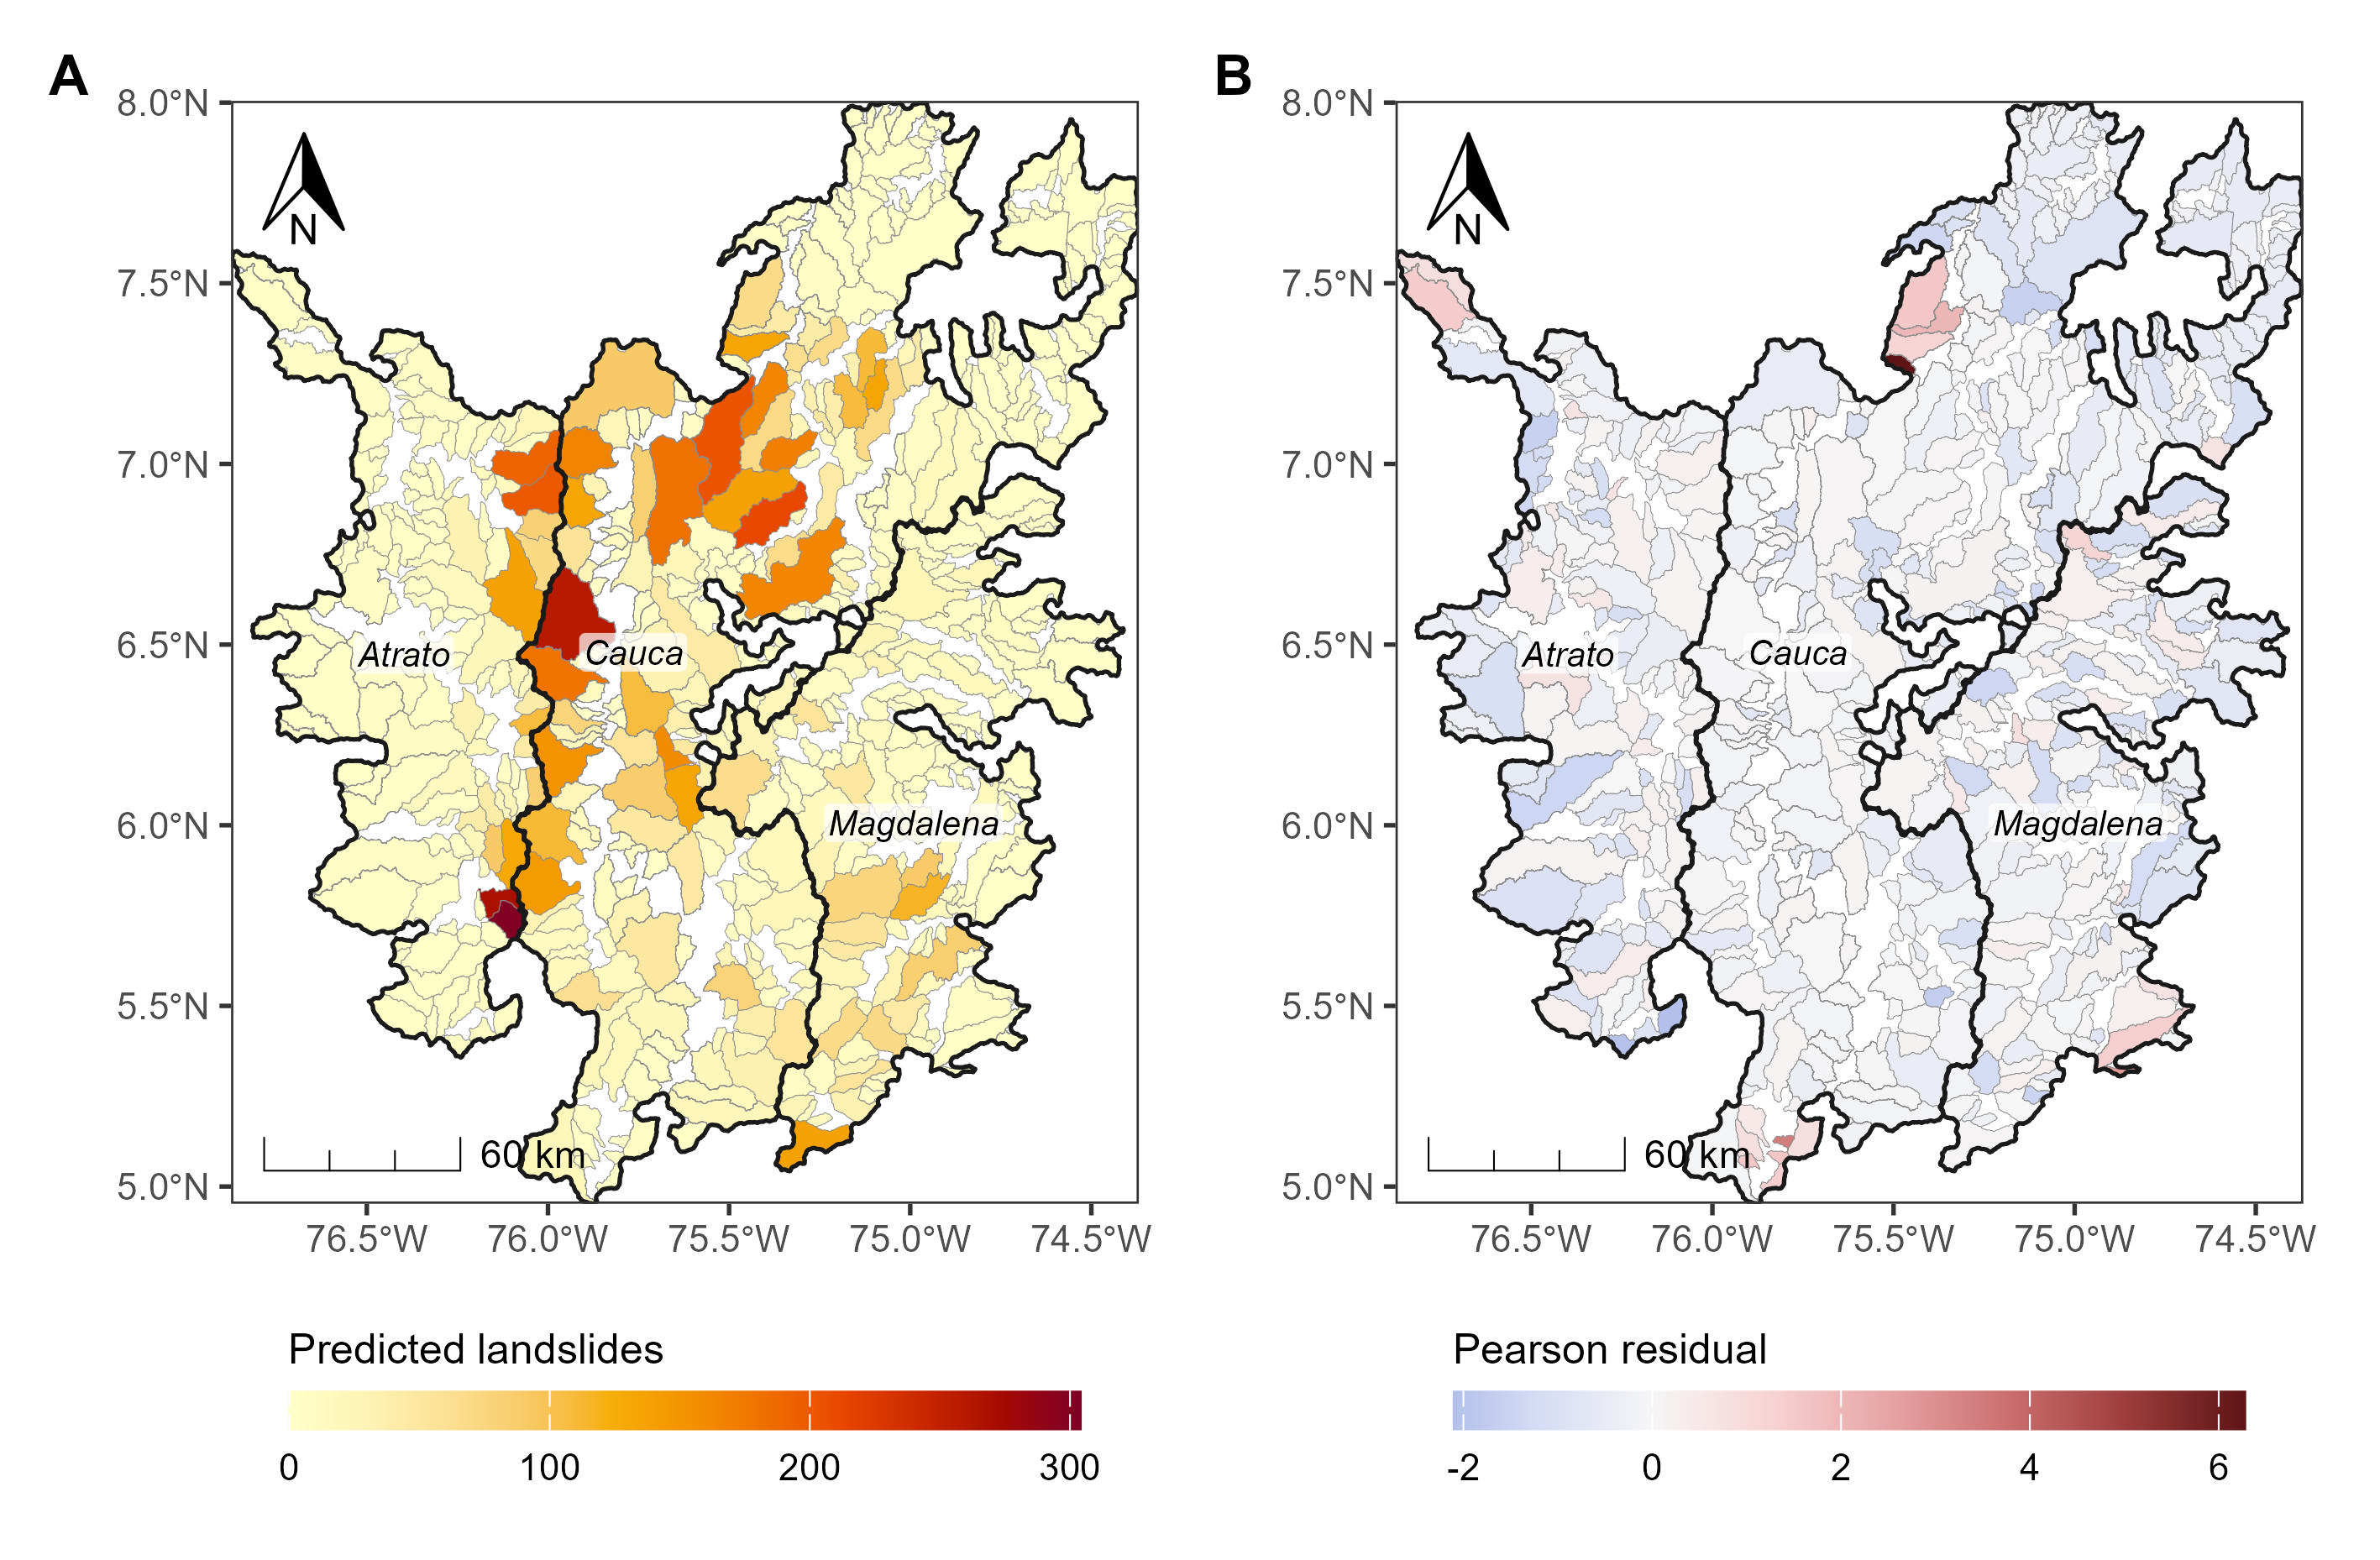
\includegraphics[width=0.8\textwidth]{Fig06_M3_icar.jpg}
\caption{Model M3 – Intrinsic Conditional Autoregressive (ICAR). (A) Predicted landslide counts using the ICAR model at the catchment level. (B) Pearson residuals after including a spatially structured random effect via an ICAR prior. \hl{The spatial pattern of residuals remains evident (MI = 0.243), indicating that the ICAR structure alone does not fully capture local spatial dependence in landslide occurrences.}}
\label{Fig6}
\end{figure}


\subsection{Model 4: Besag--York--Molli\'{e} (BYM) model}\label{subsec44}

Regarding fixed effects, all predictors have positive coefficients. 
Slope and elevation remain credibly non-zero, with posterior means of 0.742 and 0.410, respectively, in the R-INLA implementation. 
The effect of rainfall days is reduced compared to the ICAR model (now 0.139); \hl{its 95\% credible interval spans zero ([-0.13, 0.41],} \hlE{\mbox{Table~\ref{tabA3}}),} \hl{so this effect is no longer credibly distinguishable from zero once TMU-level spatial structure is included.}

\hl{The estimated precision for the TMU-level effects separates into an unstructured (iid) component (precision = 1.45, variance $\approx$ 0.69) and a spatially structured component (precision = 1.14, variance $\approx$ 0.88), both confirming residual overdispersion but markedly lower than in the ICAR-only model (variance = 3.09), reflecting how the additional unstructured term in BYM absorbs local variability that the ICAR structure alone cannot.} 
The upper-level (basin) random effects are largely attenuated in this specification, with near-zero posterior means for all three basins: Atrato (-0.001), Cauca (0.001), and Magdalena (0.000), indicating that most of the regional variation has been absorbed by the flexible structure at the TMU level.

\hl{Model fit remains favorable, with a DIC of 2551 and WAIC of 2564, the lowest among the three spatial formulations. 
The residual Moran's Index (MI) is 0.089, indicating a substantial reduction in residual spatial autocorrelation relative to M1-M3, though not its complete removal.}

\begin{figure}[h]
\centering
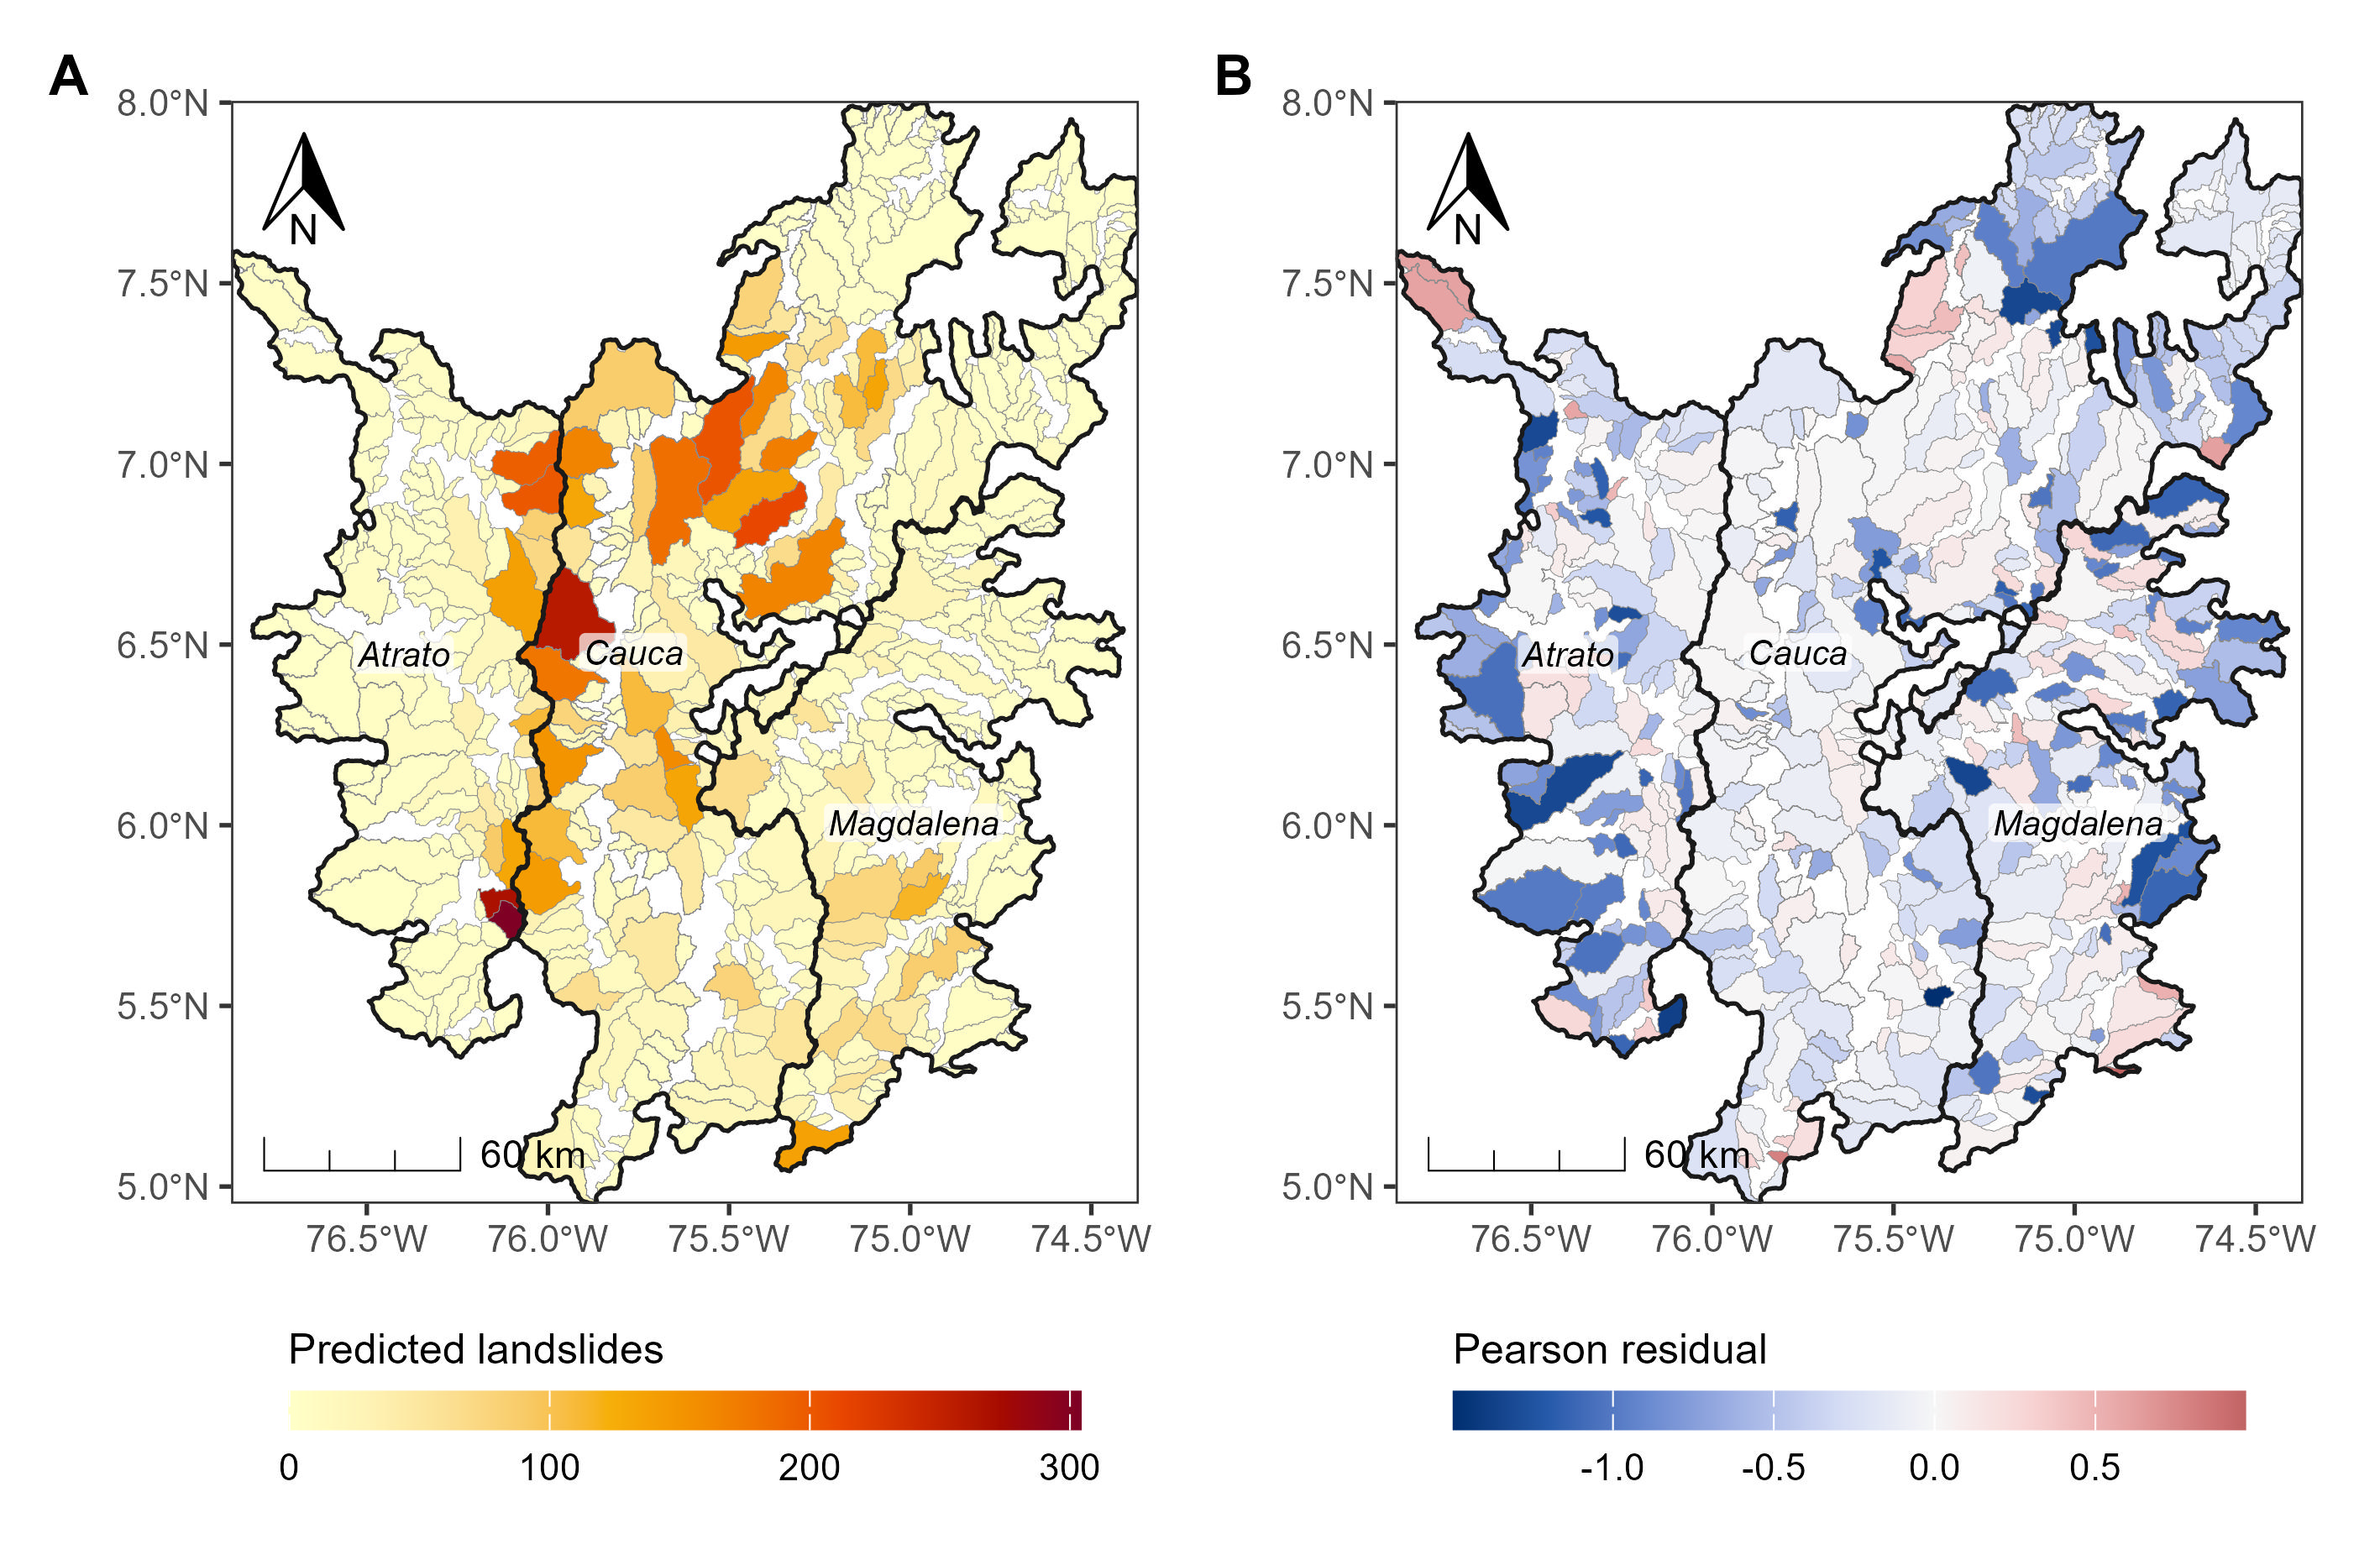
\includegraphics[width=0.8\textwidth]{Fig07_M4_bym.jpg}
\caption{Model M4 – Besag–York–Mollié (BYM). (A) Predicted landslide counts under the BYM model, which includes both structured and unstructured random effects at the TMU level. (B) \hl{Residuals show moderate spatial randomness, with most high values removed and MI reduced to 0.089.} The BYM model balances spatial smoothing and overdispersion control, improving model fit relative to ICAR.}
\label{Fig7}
\end{figure}


\subsection{Model 5: Leroux model}\label{subsec45}

The posterior estimates for the fixed effects remain credibly positive. 
Both slope and elevation retain significant contributions to landslide susceptibility, with posterior means of 0.840 and 0.652, respectively. 
In contrast, the effect of rainfall days remains low and statistically ambiguous (0.123); \hl{as in M4, its 95\% credible interval spans zero [-0.18, 0.43]}, consistent with the pattern observed in the BYM model.

\hl{The posterior mean of $\rho = 0.893$} shows a strong spatial dependency, indicating that most of the variability in the latent field is explained by the spatially structured component. 
\hlE{This indicates that the residual variation left by the predictors is dominated by a component shared among neighbouring catchments: nearly 89\% of the unexplained variability is spatially structured rather than independent.} 
\hl{This is consistent with, but does not by itself identify, unobserved spatially contiguous factors such as lithology, soil type, or fracture networks; distinguishing among these candidate drivers would require additional, explicitly geological covariates.}

The precision associated with the TMU-level effect is \hl{0.398, corresponding to a posterior variance of approximately 2.51}, which highlights a relatively high degree of overdispersion at the local level. 
\hl{The random intercepts at the basin level again show minimal influence, with posterior means near zero: Atrato (0.000), Cauca (0.000), and Magdalena (0.000), suggesting that once catchment-level spatial structure is incorporated, there is essentially no remaining variability attributable to basin-level context.}

\hl{Model fit is close to, though marginally weaker than, the BYM model on both information criteria (DIC = 2572 vs. 2551; WAIC = 2618 vs. 2564). 
However, the residual Moran's Index (MI) is} \hlE{-0.172,} \hl{the most favourable (closest to, and slightly below, zero) among the three spatial formulations, indicating that residual spatial autocorrelation is essentially eliminated under the Leroux structure.}

\begin{figure}[h]
\centering
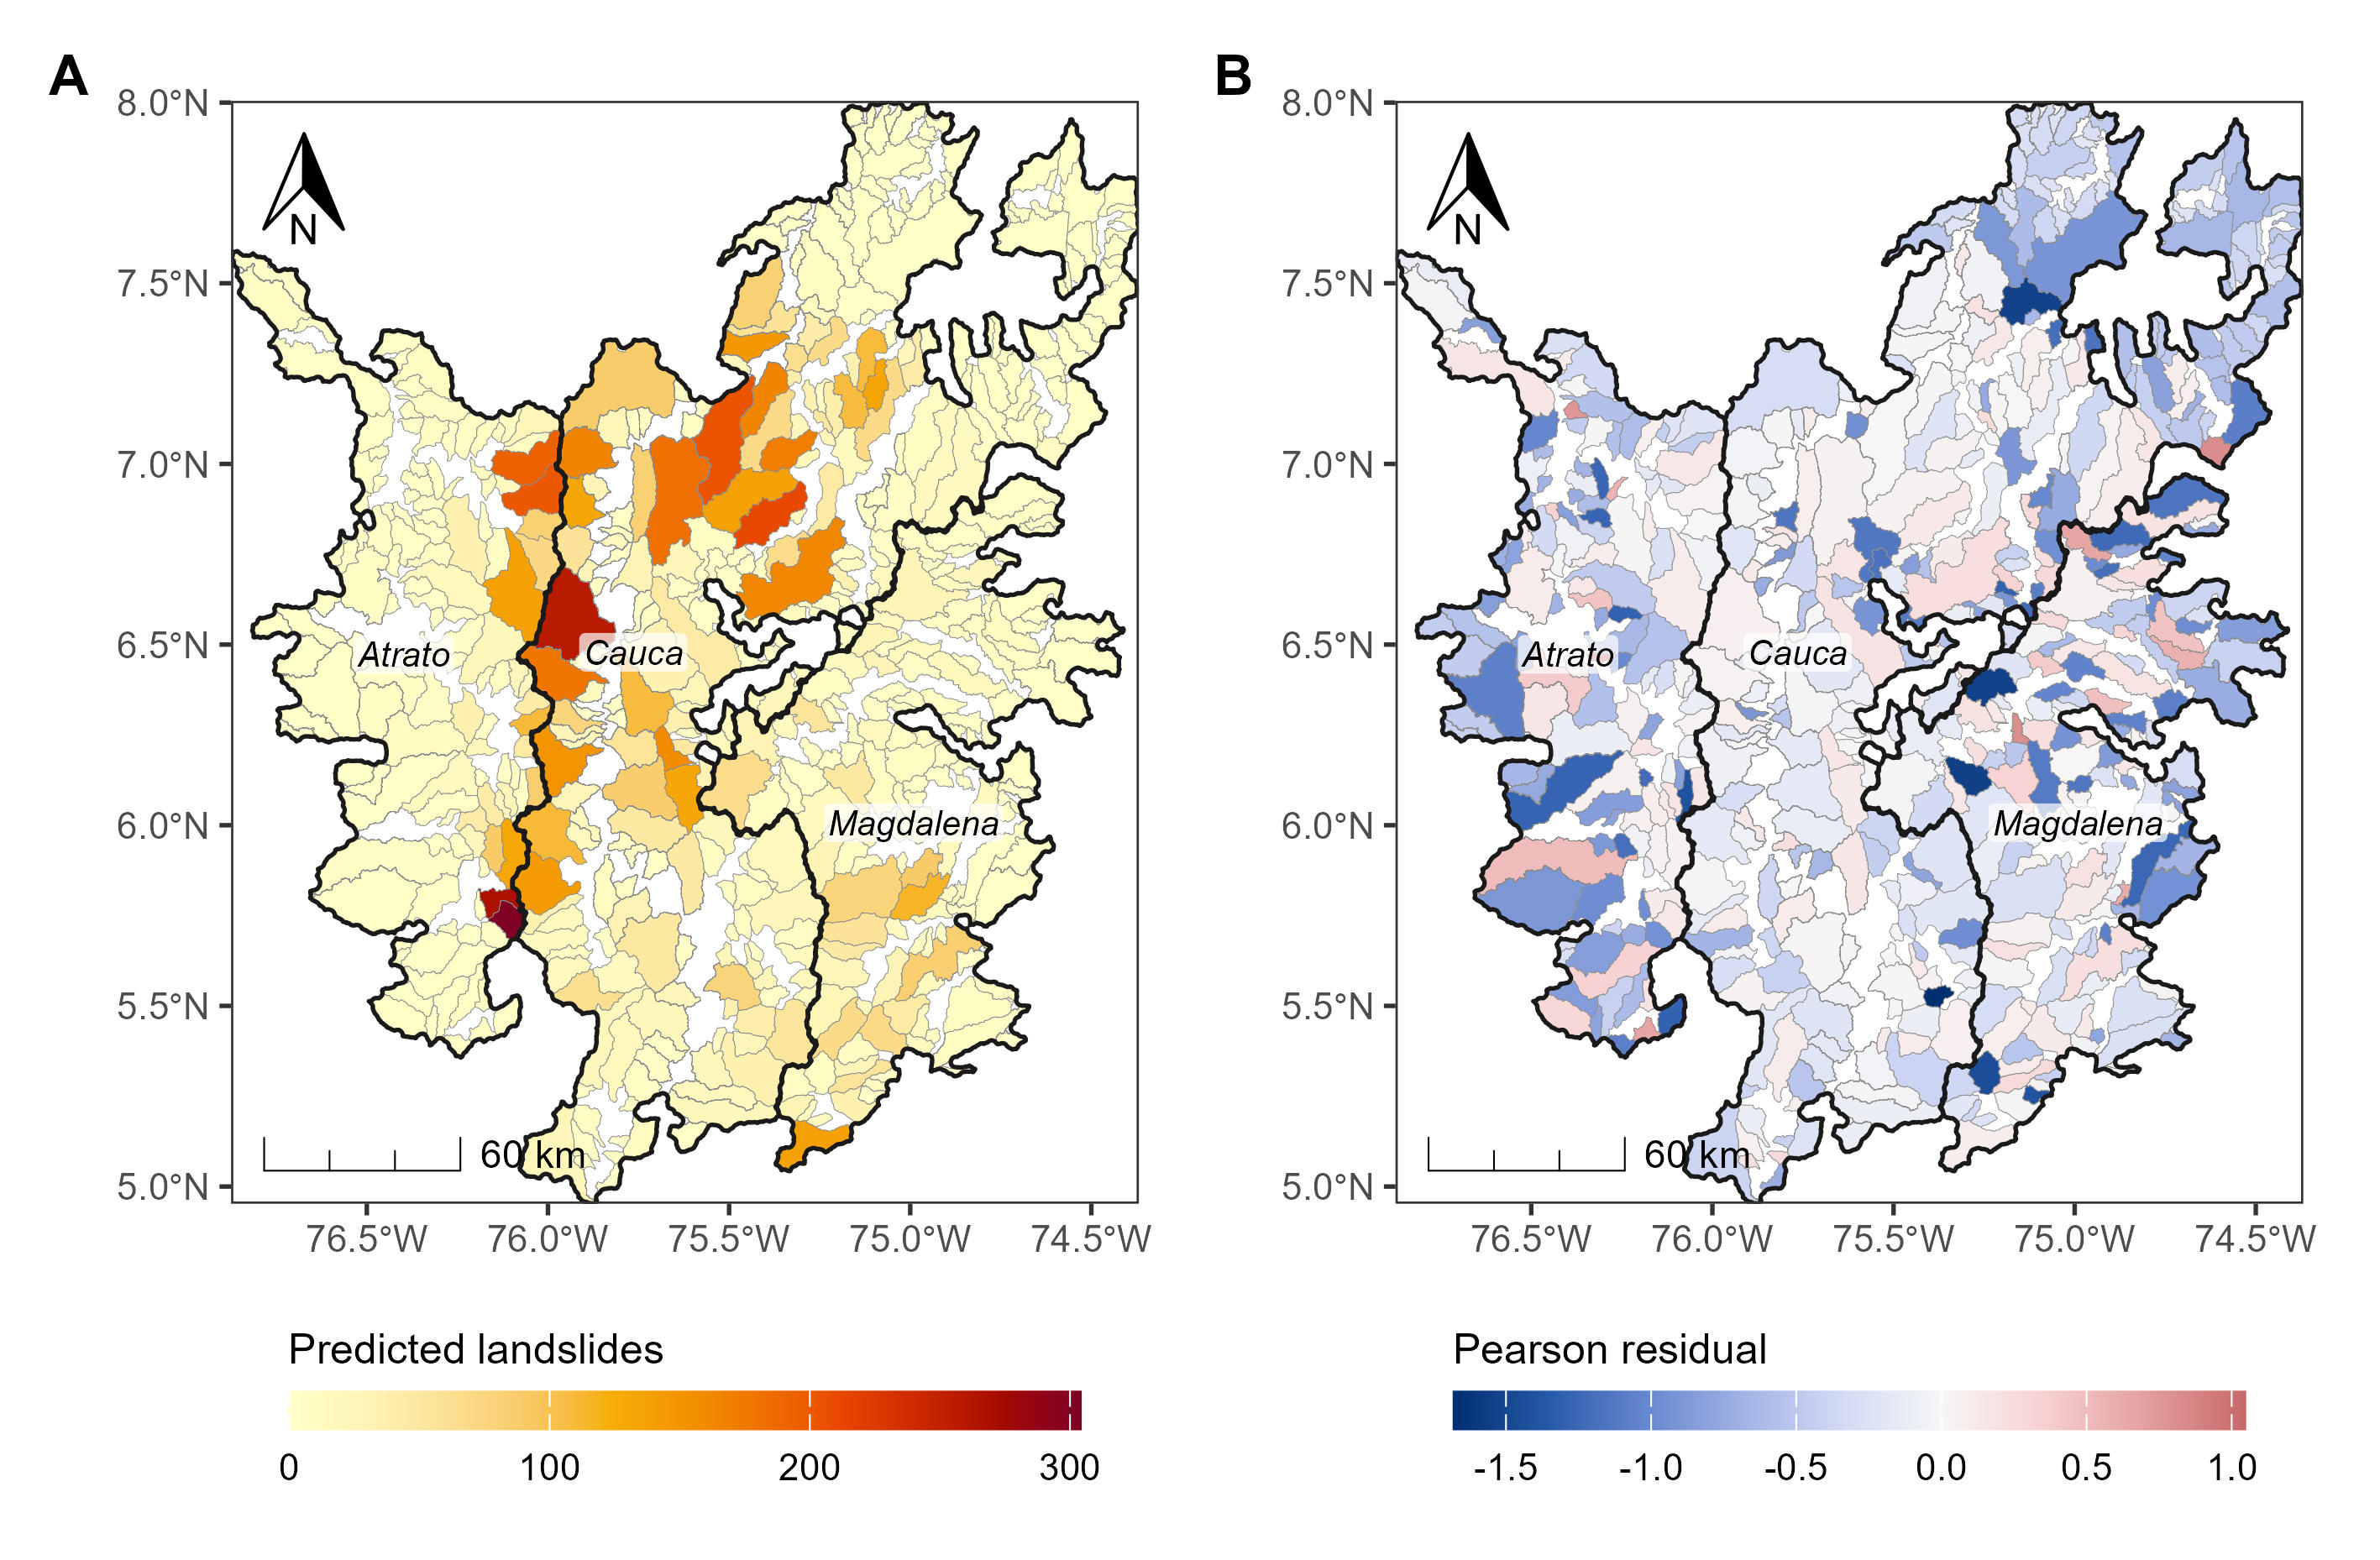
\includegraphics[width=0.8\textwidth]{Fig08_M5_leroux.jpg}
\caption{Model M5 – Leroux.(A) Predicted landslide counts from the Leroux model, which flexibly combines spatial and unstructured effects through a data-driven spatial dependency parameter \hl{($\rho$=0.893)}. (B) Pearson residuals demonstrate low residual spatial structure \hl{(MI =} \hlE{-0.172)}, confirming that the Leroux formulation effectively mitigates spatial autocorrelation while maintaining model parsimony and interpretability.}
\label{Fig8}
\end{figure}

\begin{table}[h]
\caption{Table 1. Results. Moran’s Index (MI). The inverse of the precision is the variance. \hl{All fixed-effect coefficients (M1-M5) are on standardized (mean 0, SD 1) predictors and are therefore directly comparable across models. Posterior standard deviations and 95\% credible intervals for all fixed effects are reported in} \hlE{\mbox{Appendix~\ref{secA3}} (\mbox{Table~\ref{tabA3}}).}}\label{tab1}
\begin{tabular}{@{}lccccc@{}}
\toprule
Variables & M1 & M2 & M3-ICAR & M4-BYM & M5-Leroux \\
\midrule
\textbf{Fixed Effects} & & & & & \\
Intercept & -15.551 & -15.684 & -16.856 & -16.745 & -16.750 \\
Rainfall days & 0.151 & 0.299 & 1.356 & 0.139 & 0.123 \\
Mean elevation & 0.413 & 0.485 & 0.833 & 0.410 & 0.652 \\
Mean slope & 0.617 & 0.661 & 0.729 & 0.742 & 0.840 \\
\textbf{Random Effects} & & & & & \\
Atrato & - & -0.132 & -0.515 & -0.001 & 0.000 \\
Cauca & - & 0.311 & 0.754 & 0.001 & 0.000 \\
Magdalena & - & -0.179 & -0.239 & 0.000 & 0.000 \\
$\rho$ & - & - & 1 & - & 0.893 \\
Precision TMU & - & - & 0.324 & 1.452 & 0.398 \\
Precision basins & - & 27.4 & 4.83 & 21,824 & 22,051 \\
\midrule
DIC & 10,941 & 9,469 & 2,602 & 2,551 & 2,572 \\
WAIC & 27,104 & 20,795 & 2,704 & 2,564 & 2,618 \\
MI (res) & 0.513 & 0.447 & 0.243 & 0.089 & -0.172 \\
\bottomrule
\end{tabular}
\end{table}

%%%%%%%%%%%%%%%%%%%%%%%%%%%%%%%%%%%%%%%%%%%%%%%%%%%%%%%%%%%%%%%%%%%%%%%%%%%%%%%%

\section{Discussion}\label{sec5}

\subsection{\hlE{Comparing the models}}\label{subsec51}

\hlE{We compare the models on three criteria that answer different questions and that we keep distinct throughout. DIC and WAIC measure in-sample goodness of fit, penalized for model complexity; they say nothing about performance on spatially separated data. Residual Moran's I measures whether the spatial dependence in the residuals has been absorbed, and is a diagnostic of model specification rather than of predictive skill. Spatially blocked cross-validation is the only one of the three that measures out-of-sample prediction. A model can rank highly on the first two criteria and poorly on the third, and in our case it does.}

\hl{Among the three spatial formulations, model selection criteria no longer point unanimously to a single best model. 
The BYM model (M4) achieves the lowest DIC (2551) and WAIC (2564) among M3-M5, reflecting its combination of structured and unstructured spatial components without the added complexity of estimating a mixing parameter. 
The Leroux model (M5), by contrast, achieves the lowest (most negative) residual Moran's Index} \hlE{(-0.172),} \hl{indicating that it leaves the least unexplained spatial autocorrelation among the three spatial formulations, at a small cost in DIC (2572) and WAIC (2618) relative to M4. 
The ICAR model (M3) performs worst on both criteria (DIC = 2602, WAIC = 2704, MI = 0.243), consistent with its lack of an unstructured noise term to absorb local overdispersion.}

\hl{Model selection criteria overwhelmingly favor the spatial models over the non-spatial baseline: all three spatial formulations (M3-M5) reduce DIC and WAIC by roughly three-quarters relative to M1, and reduce the residual Moran's Index from a strongly positive 0.513 to values at or below 0.24 (Table 1). 
Within this trade-off between goodness of fit (favoring M4) and residual spatial independence (favoring M5), we retain the Leroux model (M5) as our} \hlE{reference formulation for describing the in-sample spatial structure,} \hl{because it provides the most complete removal of residual spatial autocorrelation} \hlE{within the observed study area} \hl{while estimating a single, interpretable mixing parameter ($\rho = 0.893$) that separates structured from unstructured spatial variability, a property neither M3 nor M4 offers directly. 
The fixed effects remain stable and interpretable across M4 and M5, and the difference in DIC/WAIC between them (under 1\%) is small relative to the difference in residual spatial autocorrelation, which we consider the more direct diagnostic of whether the spatial dependence structure has been adequately captured.}

\hl{Residual overdispersion is substantially reduced, but not eliminated, once an unstructured noise term is included: the TMU-level posterior variance is highest for the ICAR-only model (3.09, M3), which lacks such a term, and drops to 0.69-0.88 (M4) and 2.51 (M5) once one is included (Table 1), compared with the pronounced overdispersion visible in the M1 residuals. 
This indicates that even the best-fitting models absorb, rather than fully remove, extra-Poisson variability, which is consistent with the change-of-support and missing-covariate issues and should be read as a limitation rather than as evidence that lack of fit is fully resolved.}

\hlE{The analysis of the response distribution (\mbox{Appendix~\ref{secA5}}) shows that the extra-Poisson variability in these data is spatially structured rather than independent between catchments. For the non-spatial model a negative-binomial likelihood lowers the DIC by about 7,500, but for every spatial model the same change worsens the fit (DIC from 2572 to 2956 for M5 and from 2551 to 3194 for M4): when a CAR field and an independent dispersion term are both available, they compete for the same variance, and the data prefer the spatially correlated representation. Posterior predictive checks show that M5 reproduces the total, the maximum and the variance of the counts (predicted variance 1704, 95\% interval 1570--1838, against 1690 observed), but no model, spatial or not, reproduces the number of zero-count catchments without distorting the upper tail of the distribution (M5 predicts 119, 106--133, against 144 observed). The spatial random effect also partly compensates for distributional misfit: under a negative-binomial likelihood the variance of the Leroux latent field falls by 39\%, from 2.51 to 1.53, although its spatial dominance does not diminish ($\rho$ rises from 0.894 to 0.944). The magnitude of the latent field under the Poisson likelihood should therefore be read as an upper bound, whereas its spatially structured character is robust to the choice of likelihood.}

\hlG{Because the model comparison above relies on in-sample goodness-of-fit criteria (DIC, WAIC) and residual diagnostics, we additionally assessed out-of-sample predictive performance using spatially-blocked 5-fold cross-validation, in which entire spatial neighborhoods, rather than random catchments, are held out in turn, following recommended practice for spatially structured data }\citep{brenning2005spatial}
\hlE{. This is a substantially harsher test for models that rely on local spatial smoothing to predict, since held-out catchments in the interior of a missing block have no observed neighbors to borrow strength from. }
\hlE{Under this design, the non-spatial models (M1, M2) and the BYM model (M4) predicted stably across folds (median RMSE 38.6, 43.4 and 48.3), whereas the ICAR (M3) and Leroux (M5) models, whose latent field is dominated by the structured spatial component, did not degrade gracefully but diverged: M3 reached an RMSE of $1.9 \times 10^{9}$ in fold~1 and $3.9 \times 10^{6}$ in fold~3, and M5 reached 2866 in fold~1 and 9553 in fold~5 (\mbox{Appendix~\ref{secA4}}, \mbox{Table~\ref{tabA4}}). Our in-sample ranking, in which M5 best absorbs residual autocorrelation, and our out-of-sample ranking, in which M5 is among the least reliable models, therefore disagree, and DIC and WAIC cannot adjudicate between them because both are in-sample quantities; a low residual Moran's I is likewise not evidence of predictive skill. The instability has a structural explanation: when an entire contiguous neighbourhood is withheld, a model whose latent field is dominated by the structured component has no observed neighbours from which to borrow strength, and the ICAR prior, being improper, provides no information to anchor the prediction.}

\hlE{The appropriate model therefore depends on the intended use. For retrospective explanation, for quantifying how much spatial structure the covariates fail to capture, and for spatial smoothing within the observed region, the Leroux model is the most informative. For prediction into spatially held-out catchments, or for catchment-scale zonation beyond the footprint of the inventory, BYM is the defensible choice, and the CAR-dominated specifications (M3, M5) should not be used.}

\subsection{Physical interpretation of spatial effects}\label{subsec52}

A key limitation of most hierarchical models previously used in landslide susceptibility studies is the assumption that Terrain Mapping Units (TMUs) are spatially independent. 
This simplification neglects both local spatial interactions among neighboring TMUs and regional-scale spatial heterogeneity, potentially leading to biased or incomplete representations of the underlying spatial processes.

\hl{Our findings quantify the magnitude of this residual spatial structure. 
The model} \hlE{that most fully absorbs residual spatial autocorrelation in-sample} \hl{(M5 -- Leroux) estimated the spatial autoregressive parameter, $\rho$, at 0.893, indicating that most of the unexplained variability behaves as spatially structured rather than independent among catchments. 
This shows that even after accounting for the known fixed-effect predictors (slope, elevation, rainfall), a substantial component of landslide occurrence is attributable to unobserved factors shared among neighboring catchments. 
It is important to be precise about what this result does and does not show: the CAR/ICAR/BYM/Leroux formulations encode adjacency among catchments, demonstrating that neighboring units have correlated residuals, not that this correlation stems from any specific physical process. 
Plausible sources of this structure include contiguous geological formations, soil properties, or anthropogenic disturbance not captured by our covariates, but confirming any of these would require relating the latent spatial field to independent geological or land-use data, which is beyond the scope of the present study} \citep{besag1991bayesian, lawson2018bayesian, morris2019bayesian}
\hlE{. Our results nonetheless show that omitting this spatial dependence, as standard non-spatial models do, discards a statistically influential component of the observed landslide pattern. The latent field is, moreover, conditional not only on the included covariates but also on the adjacency definition, the model specification and the chosen spatial support; it is a property of the model--data combination rather than an estimate of a physical field. Consistently, the basin-level random intercepts collapse to essentially zero once catchment-level spatial structure is included, so the grouping by basins does not by itself support an interpretation in terms of tectonic or lithological domains.}

By explicitly modeling this spatial structure (as in M3-M5), the model can disentangle these correlated effects, providing a less biased estimate of the \hlE{between-catchment association between the predictors and landslide counts}. 
For instance, the slope coefficient increased from 0.617 (M1) to \hl{0.840} (M5), and elevation from \hl{0.413 to 0.652}, suggesting the spatial confounders in the M1 model were likely acting as suppressors.

\hlE{These coefficients describe differences between catchments in their bulk terrain characteristics, not the behaviour of individual slopes, and the distinction is quantitative here. A slope-scale response estimated from within-catchment contrasts alone and integrated over each catchment implies a catchment-level slope effect about three times weaker than the one we estimate: on its original scale, the coefficient of this integrated covariate is 3.2 (95\% credible interval 2.4--3.9) in M5, against the value of 1 expected if the landslide activity of a catchment reflected only its summed slope-scale response (\mbox{Appendix~\ref{secA6}}). Catchment steepness thus also stands for correlated catchment-scale properties, such as incision, relief, regolith and hillslope--channel coupling, and possibly for spatially uneven detection (\mbox{Sect.~\ref{subsec54}}); when slope is restricted to act only through the slope-scale response, this excess is absorbed by the latent spatial field.}

The spatial models also re-allocate variance between the hierarchical levels. 
In the standard (non-spatial) multilevel model (M2), the basin-level random effects were notable (e.g., 0.311 for Cauca). 
However, once local spatial interactions among catchments are included (M3-M5), these upper-level (basin) effects decrease to near-zero, indicating that much of the variability previously attributed to basin-level context is now better explained by the local spatial structure. 
This pattern suggests that rainfall-related spatial variability is being partially absorbed by the spatial random effect, particularly in models like ICAR and Leroux that impose strong local smoothing.

\hl{These findings align with, and extend, prior evidence from both the landslide and spatial-statistics literature. }
\citet{lombardo2019geostatistical}\hl{ and }\citet{lombardo2020space}\hl{ similarly found that significant spatial dependencies persist in landslide occurrence even after including physical triggers such as rainfall or seismic shaking, consistent with our finding that a large majority (89\%) of the unexplained variability in M5 is spatially structured rather than independent. 
The magnitude of residual-autocorrelation reduction we obtain (Moran's I from 0.513 in M1 to} \hlE{-0.172} \hl{in M5) is comparable to that reported for other spatial corrections applied to landslide susceptibility models:} \citet{li2019eigenvector}\hl{, for example, reduced the residual Moran's I of a logistic regression model to 0.027 using eigenvector spatial filtering, a result of the same order of magnitude as ours despite using a markedly different spatial-correction mechanism (covariate-based filtering rather than a latent CAR field). 
The dominance of the spatially structured component over the unstructured component in our BYM and Leroux models ($\rho = 0.893$) also mirrors a common finding in the disease-mapping literature that motivated these formulations, where structured spatial variance frequently dominates unstructured heterogeneity in area-referenced count data }\citep{lawson2018bayesian, morris2019bayesian}\hl{.}

\hlE{Beyond statistical significance, the magnitude of these parameter effects has direct practical implications.} \hlE{In M5, a difference of one degree in mean catchment slope between catchments is associated with a 13.1\% difference in the expected landslide count, and a difference of 100 m in mean elevation with a 9.0\% difference. These figures are back-transformed to raw units by dividing each standardized coefficient by the standard deviation of the predictor (6.8$^{\circ}$ for slope and 756 m for elevation) before exponentiating. Because slope varies by several tens of degrees and elevation by hundreds to thousands of metres across the study area, these per-unit effects compound into several-fold differences in expected landslide frequency between low-relief and steep, high-elevation catchments. 
By contrast, the rainfall-day effect is not credibly different from zero in the two most flexible spatial models (M4, M5), and in M5 it is carried almost entirely by the five highest-count catchments: it falls from 0.122 to 0.004 (95\% credible interval $[-0.30, 0.31]$) when they are excluded from the likelihood (\mbox{Appendix~\ref{secA5}}). Our data therefore provide no evidence of a between-catchment effect of rainfall frequency once spatial structure is accounted for; this does not contradict the role of rainfall as the trigger of individual events, which a catchment-level count model cannot resolve.} 
\hlE{These results indicate that terrain morphometry, rather than the rainfall regime, is the dominant correlate of the between-catchment pattern of relative landslide susceptibility in this setting, an interpretation that would not be apparent from the coefficients' statistical significance alone.}

\subsection{Implications for susceptibility zonation}\label{subsec53}

These findings have direct implications for the practice of landslide susceptibility zonation. 
A traditional, non-spatial model (like M1) produces a patchy map, where susceptibility is driven only by the local predictors. 
This map would fail to capture the cohesive, higher-susceptibility zones \hlE{where landslide activity is spatially clustered}. 
Our spatial HGLM (M5), by incorporating the $\rho$ parameter, effectively listens to the neighboring catchments. 
\hlE{The resulting fitted surface is smoother, which is a consequence of the CAR prior rather than evidence of predictive quality, and it propagates information across contiguous catchments that share residual structure.} 
\hl{This produces more spatially coherent zones of high susceptibility (e.g., in the Cauca basin) than a non-spatial model would, offering a more defensible basis for land-use planning; validating these zones against independent geological or geotechnical data remains a task for future work.} \hlE{The resolution of this zonation is set by the spatial support: the map assigns one value to each catchment (median area 48.7~km$^2$) and therefore cannot distinguish susceptible from stable slopes within a catchment, and its use beyond the inventory footprint is limited by the cross-validation results of \mbox{Sect.~\ref{subsec51}}.} 
\hlG{Recent work has also emphasized the value of jointly visualizing susceptibility and its associated uncertainty, rather than reporting point estimates alone }\citep{schlogl2025visualizing}\hlG{; extending our credible-interval-based uncertainty quantification into a bivariate susceptibility-uncertainty map is a natural next step for this framework.}

\subsection{\hl{Limitations}}\label{subsec54}

\hl{This inventory has limitations relevant to its completeness and consistency. 
It was compiled by a single interpreter without a formal, independent quality-control or cross-validation step, which introduces some subjectivity in landslide delineation and detection thresholds. 
The availability of sub-metre optical imagery in Google Earth Pro is also uneven over this 53-year record and across the three basins, becoming systematically sparser before approximately the early 2000s and varying in coverage between the Atrato, Cauca, and Magdalena basins; this is a common source of spatially and temporally uneven detection in visually-mapped regional inventories }\citep{loche2022landslide}\hl{, and likely biases our inventory toward more recent, better-imaged events and areas. 
We did not compile individual landslide areas and therefore could not assess completeness for small landslides through a magnitude-frequency} \hlE{analysis} \citep{malamud2004landslide, tanyas2020completeness}\hlE{; the inventory has therefore not been subjected to a formal completeness assessment.}

\hl{Because hierarchical spatial models explicitly borrow information between neighboring units, any bias in the underlying inventory is not confined to the catchments where it originates: uneven detection or interpreter inconsistency in one catchment propagates, through the latent spatial field, into the fitted values of its neighbors. 
Spatial models are therefore more sensitive to inventory quality than non-spatial ones, which treat each catchment independently. 
This makes a detailed, catchment-level inventory such as the one compiled here particularly important, since a coarser or more heterogeneously mapped inventory would be expected to propagate its inconsistencies more broadly across the fitted susceptibility surface.}

\hlE{The latent field may also partly represent this bias rather than merely propagate it. The drivers of uneven detection in a visually mapped inventory, namely imagery date and resolution, cloud cover, vegetation density and terrain visibility, are themselves spatially autocorrelated at roughly the scale at which the CAR field operates, and a model cannot distinguish a spatially structured excess of landslides from a spatially structured excess of detected landslides. The magnitude of the latent field is therefore an upper bound on the spatially structured process signal, not an estimate of it.}

\hlE{Aggregation to catchments discards about two thirds of the within-study-area variability of slope (\mbox{Appendix~\ref{secA6}}). Although this does not affect the modelled counts or their latent structure, restricting the aggregation of predictors to the terrain that can plausibly host or receive the process, i.e.~to potential process areas }\citep{steger2026dynamic}\hlE{, rather than averaging over whole catchments including valley floors and ridge crests, would be a more principled route, and the one we would adopt at slope-unit support. Finally, no likelihood we tested reproduces the number of landslide-free catchments without distorting the upper tail of the count distribution (\mbox{Appendix~\ref{secA5}}); this systematic under-prediction of zero counts remains an open problem of the specification.}

\hl{For the same reason, the spatial models developed here should not be extrapolated to catchments lacking nearby inventoried landslides. 
As shown by the spatially-blocked cross-validation, the spatial patterns captured by the CAR-based models are not homogeneous across the study area but specific to each basin and its immediate surroundings; prediction for new, unsampled areas is consequently limited to regions reasonably close to the existing inventory, rather than to the northern Colombian Andes as a whole.}

\section{Conclusion}\label{sec6}

This study underscores the critical need to incorporate spatial hierarchical models in landslide susceptibility mapping. 
Landslide susceptibility is inherently a spatial process, and traditional models often fail to account for the spatial dependence and heterogeneity present in geospatial data, \hl{leading to biased coefficient estimates and residual spatial autocorrelation that standard diagnostics can detect but non-spatial models cannot resolve.}

\hlE{Our results show that latent spatial effects account for a large share of the within-study-area residual structure in catchment-scale landslide counts, and that the extra-Poisson variability of these counts is itself spatially structured rather than independent between catchments.} 
By integrating spatial dependency effects and spatial heterogeneity, these models address the limitations of standard multilevel models. 
The incorporation of MRF models, such as ICAR, BYM, and Leroux, allows for a detailed representation of spatial relationships.

\hlE{Ignoring this structure biases the fixed-effect estimates, which are between-catchment associations, and produces overconfident intervals. However, strongly CAR-dominated specifications have limited transferability: under spatially blocked cross-validation they become unstable when a contiguous neighbourhood is unobserved, and BYM is the more defensible choice where prediction into unobserved catchments is the objective. The spatial HGLMs yield more spatially coherent fitted surfaces and better-calibrated within-sample uncertainty than their non-spatial counterpart, but smoothness is a property of the CAR prior rather than evidence of predictive accuracy, and the magnitude of the latent field is an upper bound on the spatially structured process signal, because it may also reflect uneven landslide detection.}

\codedataavailability{Data and code used for this study are fully available in Github (https://github.com/edieraristizabal/PAPER\_BHGLM).} %% use this section when having data sets and software code available

%%%%%%%%%%%%%%%%%%%%%%%%%%%%%%%%%%%%%%%%%%%%%%%%%%%%%%%%%%%%%%%%%%%%%%%%%%%%%%%%
%% APPENDIX A -- Supplementary analyses (new in the revision)
%% Tables are inserted from Copernicus/REV/appendix/tabA*.tex, which are
%% generated by CODES/appendix_material.R from the archived outputs.
%%%%%%%%%%%%%%%%%%%%%%%%%%%%%%%%%%%%%%%%%%%%%%%%%%%%%%%%%%%%%%%%%%%%%%%%%%%%%%%%
\appendix
\section{\hlE{Supplementary analyses}}\label{secA}
\appendixfigures
\appendixtables

This appendix documents the data, methods and results of the supplementary analyses referred to in the main text. Unless stated otherwise, every analysis uses the same 526 catchments, Queen adjacency, standardized predictors and $\log(A_i)$ offset as models M1--M5 (Sect.~\ref{sec3}), and residual Moran's I is computed as in Eq.~(\ref{eq:moran}). All analyses are reproducible with the scripts in the code repository.

\subsection{Spatial support: catchments, inventory and terrain data}\label{secA1}

The 10\,837 landslides are represented by the point locations of their crowns. Terrain statistics were computed from the 12.5~m ALOS-PALSAR DEM used for the terrain predictors (Sect.~\ref{sec3}); slope was calculated with an eight-neighbour (Horn) finite-difference scheme, and each 12.5~m cell was assigned to the catchment containing its centre. Recomputing the catchment-mean slope and elevation in this way reproduces the predictors used in the models ($r > 0.9999$), so all analyses in this appendix share their support with the main models.

The catchments have a median area of 48.7~km$^2$ (range 15.1--577.3~km$^2$). The landslide counts are strongly right-skewed: 144 catchments (27.4\%) contain no mapped landslide, the median count is 4, the mean 20.6 and the maximum 304 (Table~\ref{tabA1}, Fig.~\ref{figA1}). The within-catchment standard deviation of slope (median 9.7$^{\circ}$) is larger than the standard deviation of the catchment means themselves (6.8$^{\circ}$), which anticipates the result of Sect.~\ref{secA6} that most of the slope variability in the study area lies within, not between, catchments.

\begin{table}[h]
\caption{Descriptive statistics of the 526 catchments. Terrain statistics computed from the 12.5~m ALOS-PALSAR DEM; within-catchment standard deviations (SD) quantify the variability that aggregation to catchment means discards.}\label{tabA1}
\footnotesize
\begin{tabular}{@{}lrrrrrr@{}}
\toprule
Variable & Min & Q1 & Median & Mean & Q3 & Max \\
\midrule
Catchment area (km$^2$) & 15.1 & 27.3 & 48.7 & 83.4 & 110.6 & 577.3 \\
Mapped landslides & 0 & 0 & 4 & 20.6 & 19 & 304 \\
Rainfall days, $R_d$ & 296 & 1,344 & 2,039 & 2,173 & 2,890 & 6,148 \\
Mean elevation, $H$ (m) & 32 & 688 & 1,305 & 1,315 & 1,881 & 3,161 \\
Within-catchment SD of elevation (m) & 5 & 138 & 237 & 271 & 383 & 771 \\
Mean slope, $S$ ($^{\circ}$) & 1.4 & 14.8 & 18.8 & 19.1 & 24.6 & 36.9 \\
Within-catchment SD of slope ($^{\circ}$) & 1.9 & 8.7 & 9.7 & 9.5 & 10.7 & 15.3 \\
\bottomrule
\end{tabular}
\end{table}

\begin{figure}[h]
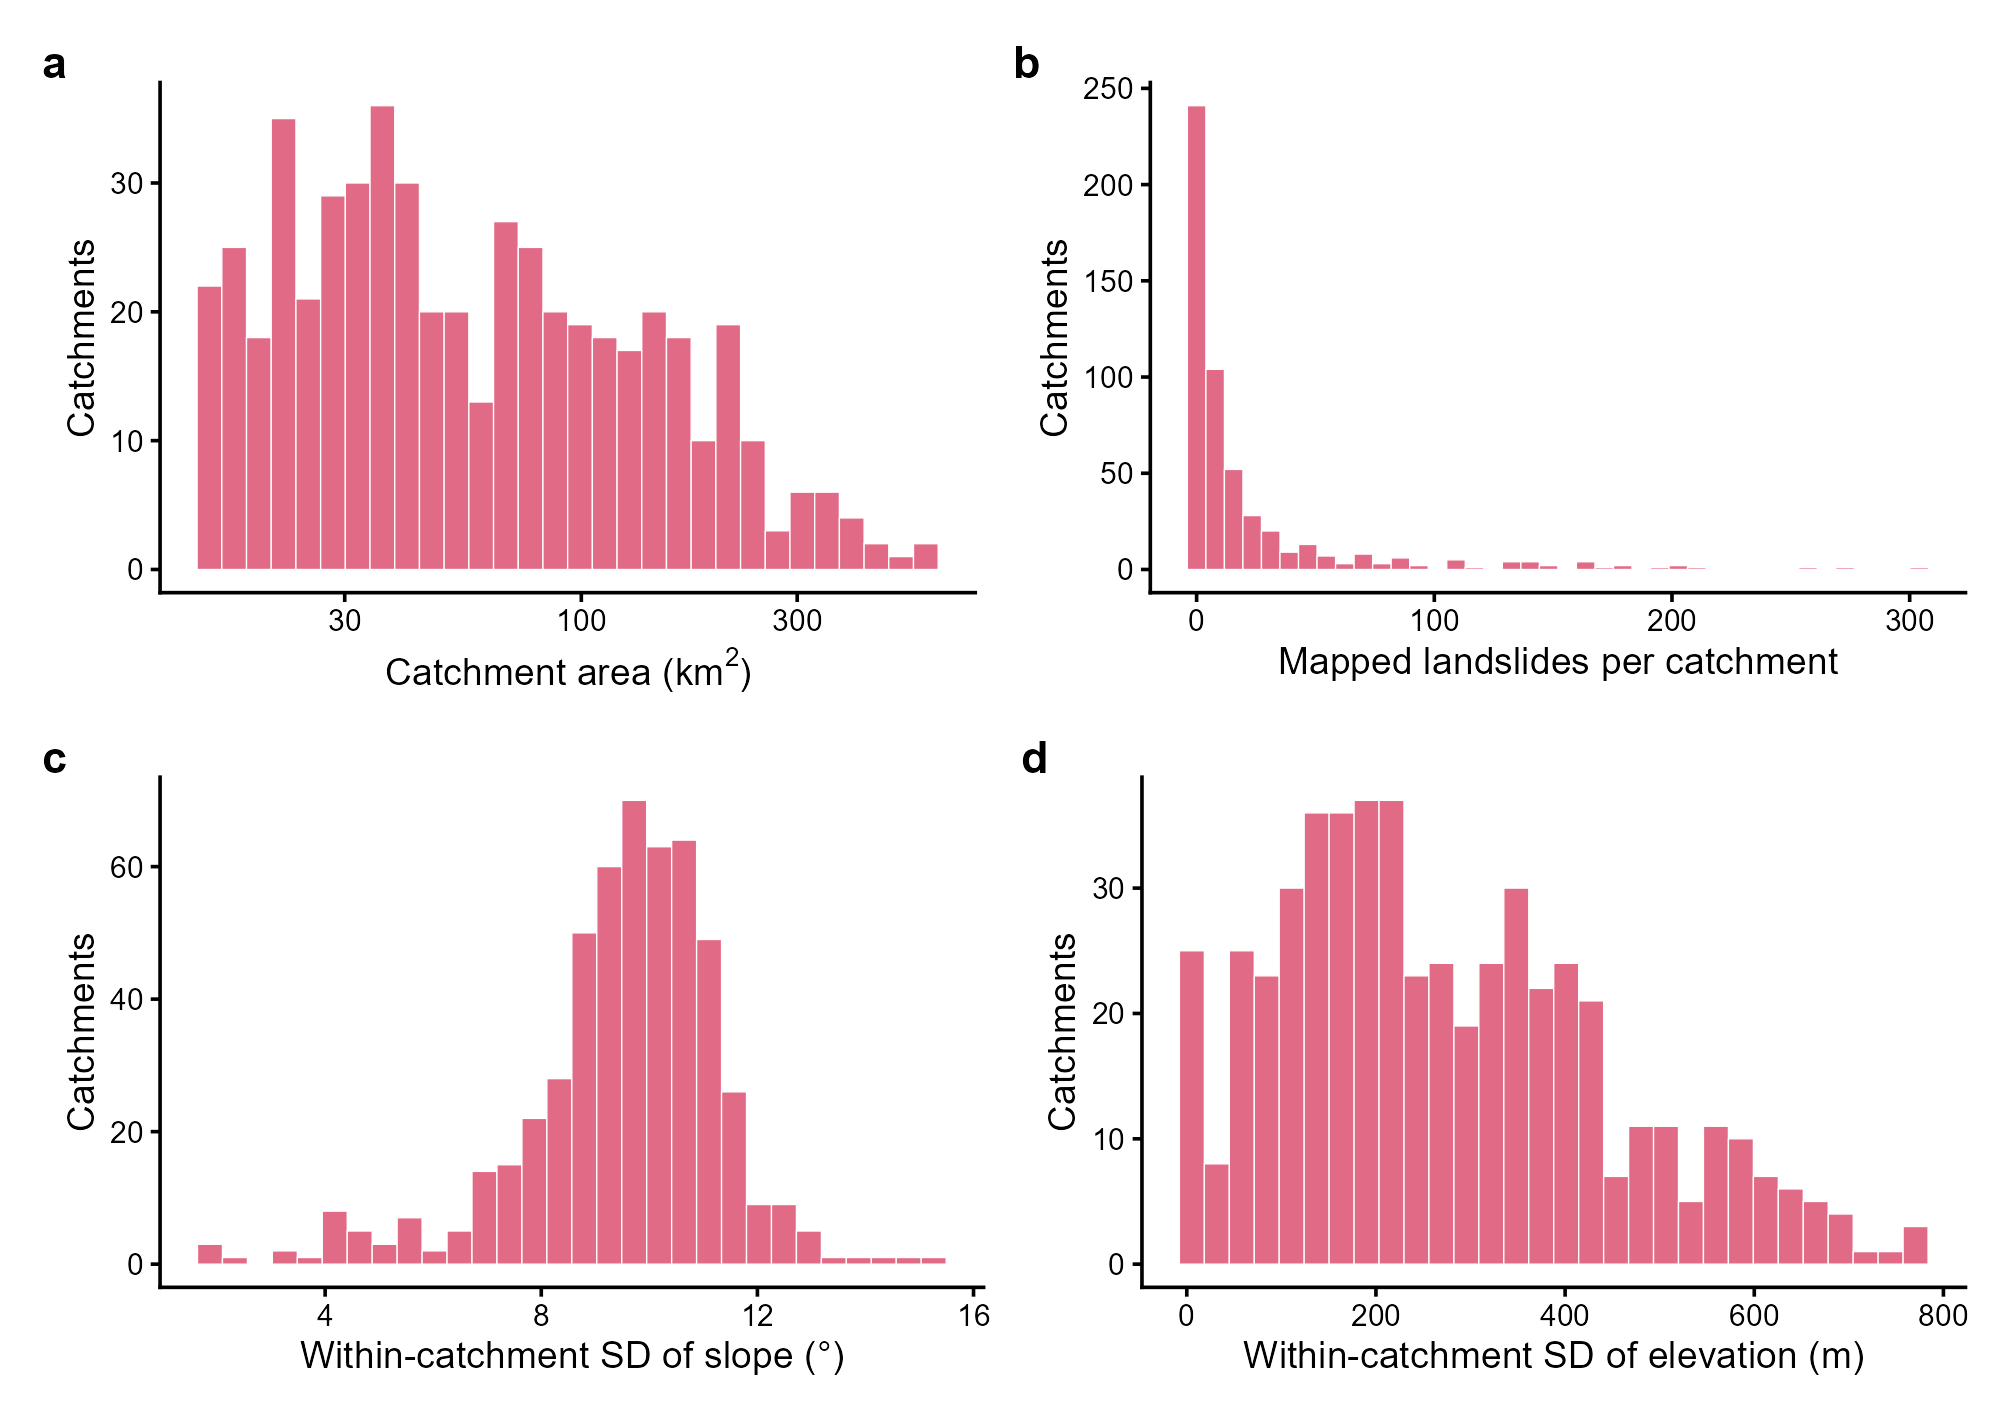
\includegraphics[width=\textwidth]{FigA1_spatial_support.png}
\caption{Spatial support of the models. Distributions across the 526 catchments of (a) catchment area (logarithmic axis), (b) the number of mapped landslides, (c) the within-catchment standard deviation of slope and (d) the within-catchment standard deviation of elevation, both computed from the 12.5~m DEM.}\label{figA1}
\end{figure}

\subsection{Predictor screening and linearity}\label{secA2}

Candidate predictors were screened with pairwise Pearson correlations; a predictor was excluded if $|r| > 0.75$ with a retained predictor (Sect.~\ref{sec3}). The full correlation matrix is given in Table~\ref{tabA2}. Linearity of the predictor--response relation was tested in the M1 specification by adding a quadratic term for each predictor in turn and, for slope, a penalized spline, and comparing the fits by AIC and likelihood-ratio tests. The partial-residual plot for mean slope (Fig.~\ref{figA2}) shows the concave departure from linearity reported in Sect.~\ref{sec3}.

\begin{table*}[h]
\caption{Pearson correlation matrix of the candidate catchment-level predictors. Values with $|r| > 0.75$, the multicollinearity threshold, are in bold. $R_d$: days with rainfall $>$20~mm; $H$: mean elevation; $S$: mean slope; TWI: topographic wetness index; Curv.: curvature index; DD: drainage density; HI: hypsometric integral; LD: lineament density; Rel.: mean relief; MAR: mean annual rainfall.}\label{tabA2}
\footnotesize
\begin{tabular}{@{}lrrrrrrrrrrr@{}}
\toprule
& $R_d$ & $H$ & $S$ & TWI & Curv. & DD & Area & HI & LD & Rel. & MAR \\
\midrule
$R_d$ & 1 &  &  &  &  &  &  &  &  &  &  \\
$H$ & -0.64 & 1 &  &  &  &  &  &  &  &  &  \\
$S$ & -0.32 & 0.57 & 1 &  &  &  &  &  &  &  &  \\
TWI & 0.31 & -0.59 & \textbf{-0.80} & 1 &  &  &  &  &  &  &  \\
Curv. & 0.04 & 0.01 & 0.04 & -0.00 & 1 &  &  &  &  &  &  \\
DD & 0.06 & -0.15 & -0.12 & 0.15 & -0.05 & 1 &  &  &  &  &  \\
Area & -0.00 & 0.07 & -0.01 & -0.00 & -0.03 & 0.11 & 1 &  &  &  &  \\
HI & -0.34 & 0.38 & 0.37 & -0.39 & 0.07 & -0.09 & -0.07 & 1 &  &  &  \\
LD & -0.20 & 0.47 & \textbf{0.91} & -0.74 & 0.10 & -0.09 & -0.11 & 0.34 & 1 &  &  \\
Rel. & -0.33 & 0.54 & \textbf{0.96} & \textbf{-0.75} & 0.04 & -0.14 & 0.01 & 0.38 & \textbf{0.81} & 1 &  \\
MAR & \textbf{0.98} & -0.62 & -0.29 & 0.28 & 0.03 & 0.08 & 0.01 & -0.35 & -0.17 & -0.29 & 1 \\
\bottomrule
\end{tabular}
\end{table*}

\begin{figure}[h]
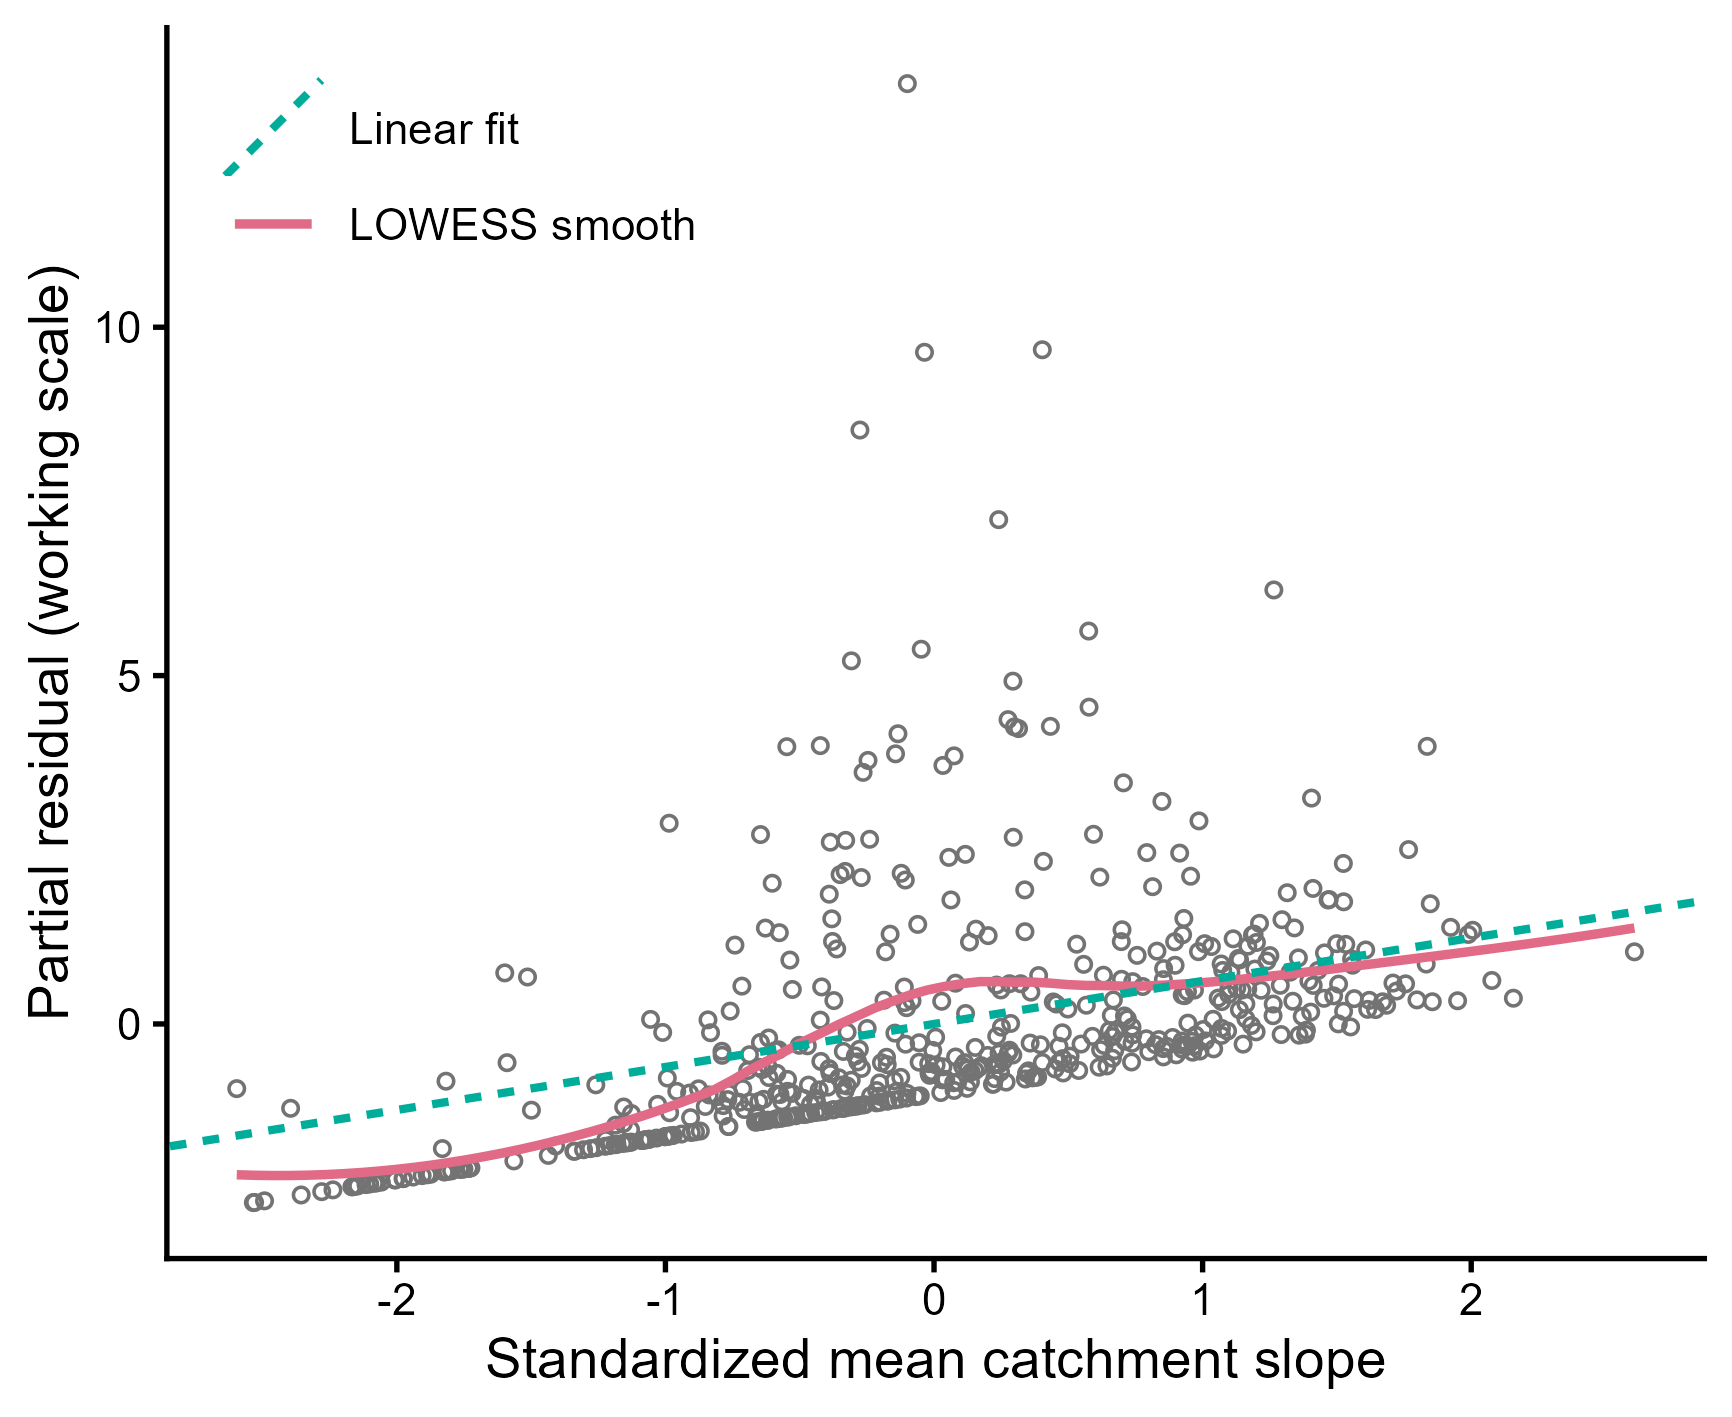
\includegraphics[width=0.6\textwidth]{FigA2_slope_partial_residual.png}
\caption{Partial-residual plot for standardized mean catchment slope in the M1 baseline, with a LOWESS smooth (solid) and the linear fit (dashed).}\label{figA2}
\end{figure}

\subsection{Posterior summaries of the fixed effects}\label{secA3}

Table~\ref{tabA3} reports the posterior mean, posterior standard deviation and 95\% credible interval (2.5\% and 97.5\% posterior quantiles, from the INLA marginals) of every fixed effect in M1--M5.

\begin{table*}[h]
\caption{Posterior mean (posterior standard deviation) and 95\% credible interval of the fixed effects in M1--M5, on standardized predictors (mean 0, SD 1).}\label{tabA3}
\footnotesize
\begin{tabular}{@{}lccccc@{}}
\toprule
Term & M1 & M2 & M3-ICAR & M4-BYM & M5-Leroux \\
\midrule
Intercept & -15.551 (0.013) & -15.684 (0.142) & -16.856 (0.356) & -16.745 (0.077) & -16.750 (0.241) \\
 & [-15.576,\, -15.525] & [-15.975,\, -15.394] & [-17.587,\, -16.144] & [-16.897,\, -16.597] & [-17.253,\, -16.293] \\
Rainfall days & 0.151 (0.013) & 0.299 (0.015) & 1.356 (0.115) & 0.139 (0.135) & 0.123 (0.154) \\
 & [0.125,\, 0.176] & [0.269,\, 0.328] & [1.131,\, 1.584] & [-0.125,\, 0.405] & [-0.178,\, 0.427] \\
Mean elevation & 0.413 (0.015) & 0.485 (0.016) & 0.833 (0.128) & 0.410 (0.119) & 0.652 (0.129) \\
 & [0.382,\, 0.443] & [0.454,\, 0.517] & [0.583,\, 1.086] & [0.178,\, 0.643] & [0.400,\, 0.905] \\
Mean slope & 0.617 (0.013) & 0.661 (0.013) & 0.729 (0.094) & 0.742 (0.091) & 0.840 (0.106) \\
 & [0.592,\, 0.642] & [0.635,\, 0.687] & [0.545,\, 0.915] & [0.565,\, 0.920] & [0.633,\, 1.048] \\
\bottomrule
\end{tabular}
\end{table*}

\subsection{Spatially blocked cross-validation}\label{secA4}

Catchments were grouped into five geographically compact folds by $k$-means clustering of their centroids ($k = 5$, 25 random starts), so that each fold withholds a contiguous neighbourhood rather than scattered catchments \citep{brenning2005spatial}. For each fold, the counts of the held-out catchments were set to missing, the model was refitted with the full adjacency graph, and the posterior mean of the fitted count in each held-out catchment was compared with the observed count by the root-mean-square error (RMSE). Table~\ref{tabA4} gives the RMSE per fold. M1, M2 and M4 are stable across folds (median RMSE 38.6, 43.4 and 48.3), whereas the ICAR (M3) and Leroux (M5) models diverge in the folds in which a large contiguous neighbourhood is entirely unobserved: M3 reaches an RMSE of $1.9 \times 10^{9}$ in fold~1, and M5 reaches 2866 and 9553 in folds 1 and 5.

\begin{table}[h]
\caption{Spatially blocked 5-fold cross-validation: root-mean-square error (RMSE) of the predicted landslide counts in the held-out catchments of each fold. Folds are geographically compact groups of catchments obtained by $k$-means clustering of catchment centroids.}\label{tabA4}
\footnotesize
\begin{tabular}{@{}ccrrrrr@{}}
\toprule
Fold & $n$ & M1 & M2 & M3-ICAR & M4-BYM & M5-Leroux \\
\midrule
1 & 98 & 38.6 & 43.4 & $1.9 \times 10^{9}$ & 67.6 & 2,866.3 \\
2 & 96 & 41.2 & 50.0 & 173.2 & 117.6 & 120.8 \\
3 & 125 & 22.9 & 22.2 & $3.9 \times 10^{6}$ & 24.4 & 20.5 \\
4 & 110 & 34.6 & 34.6 & 61.2 & 30.0 & 32.9 \\
5 & 97 & 47.4 & 47.9 & 169.7 & 48.3 & 9,552.8 \\
\midrule
Median & & 38.6 & 43.4 & 173.2 & 48.3 & 120.8 \\
\bottomrule
\end{tabular}
\end{table}

\subsection{Response distribution and model diagnostics}\label{secA5}

\textit{Methods.} We assessed whether the Poisson likelihood is adequate in four steps. (i) Marginal overdispersion was measured by the variance-to-mean ratio of the counts, and zero inflation by comparing the observed number of zero-count catchments with the number expected under a Poisson distribution with the observed marginal mean. (ii) M1, M4 and M5 were refitted under negative-binomial, zero-inflated Poisson, zero-inflated negative-binomial and hurdle likelihoods, with everything else unchanged. (iii) Posterior predictive checks were computed from 500 joint posterior samples of each model; for each sample a replicated dataset was drawn from the likelihood, and four statistics were compared with their observed values: the total count, the number of zero-count catchments, the maximum count and the variance of the counts. The Bayesian $p$-value is the proportion of replicates in which the statistic equals or exceeds its observed value. (iv) The sensitivity to influential catchments was assessed by refitting M5 with the counts of the five highest-count catchments set to missing, so that they are excluded from the likelihood but retained in the adjacency graph. Finally, the Leroux latent field was compared between the Poisson and negative-binomial likelihoods, to assess whether the spatial random effect compensates for response-distribution misspecification.

\textit{Results.} The counts are strongly overdispersed: the variance is 1689.8 against a mean of 20.6, a variance-to-mean ratio of 82.0, and the 144 zero-count catchments compare with an expectation of the order of $10^{-6}$ under a Poisson distribution with the observed mean. For the non-spatial model, replacing the Poisson by a negative-binomial likelihood lowers DIC from 10\,941 to 3\,453; for the spatial models, the same change raises DIC, from 2\,572 to 2\,956 for M5 and from 2\,551 to 3\,194 for M4 (Table~\ref{tabA5}). Consistently, the negative-binomial size parameter increases from 0.58 in M1 to 4.2 in M5, i.e.\ most of the extra-Poisson variability that the negative binomial represents as independent catchment-level dispersion is represented by the Leroux model as spatially correlated variability.

The posterior predictive checks (Fig.~\ref{figA3}) show that M1 with a Poisson likelihood fails on two of the four statistics: it predicts 21.5 zero-count catchments (95\% interval 14--29) against 144 observed, and a count variance of 918 (850--992) against 1690 ($p < 0.002$ in both cases). M5 with a Poisson likelihood reproduces the total count, the maximum count (305; 268--352, against 304) and the count variance (1704; 1570--1838, $p = 0.58$). No model, however, reproduces the number of zero-count catchments: M5 predicts 119 (106--133; $p < 0.002$), M4 121 ($p = 0.002$), M5 with a negative-binomial likelihood 124 ($p = 0.006$) and M5 with a zero-inflated negative-binomial likelihood 127 ($p = 0.024$). Only the non-spatial negative binomial reaches the observed value (129; 104--153, $p = 0.11$), at the cost of a predicted maximum of 1007 (419--2300) and a predicted variance of 6590 (2233--18\,186).

Excluding the five highest-count catchments (203, 213, 259, 270 and 304 landslides) from the likelihood leaves the latent structure of M5 essentially unchanged: on the 521 remaining catchments residual Moran's I moves from $-0.176$ to $-0.182$, $\rho$ from 0.894 to 0.901 and the latent-field variance from 2.51 to 2.40. The slope and elevation effects change from 0.841 to 0.802 and from 0.653 to 0.580, whereas the rainfall-day effect falls from 0.122 to 0.004 (95\% credible interval $[-0.297, 0.307]$).

Under the negative-binomial likelihood the variance of the Leroux latent field falls from 2.51 to 1.53, a reduction of 39\%, while its spatial dominance increases ($\rho$ from 0.894 to 0.944) and the standard deviation of the fitted latent field falls by only 7\%, from 1.41 to 1.30. Part of the latent-field variance in the Poisson model therefore reflects distributional misfit, but the structured spatial component persists, and is preferred by DIC, when the likelihood is free to absorb dispersion independently.

\begin{table}[h]
\caption{Model comparison under alternative count likelihoods. All specifications share the predictors, Queen adjacency and $\log(A_i)$ offset of the main models. MI: residual Moran's I (Eq.~\ref{eq:moran}); max $|r|$: largest absolute Pearson residual.}\label{tabA5}
\footnotesize
\begin{tabular}{@{}lrrrr@{}}
\toprule
Specification & DIC & WAIC & MI & max $|r|$ \\
\midrule
M1, Poisson & 10,941 & 27,104 & 0.513 & 35.3 \\
M1, negative binomial & 3,453 & 3,454 & 0.555 & 35.0 \\
M1, zero-inflated Poisson & 9,740 & 31,962 & 0.500 & 33.5 \\
M1, zero-inflated neg.\ binomial & 3,455 & 3,455 & 0.553 & 34.6 \\
M1, hurdle Poisson & 9,757 & 31,822 & 0.499 & 33.7 \\
M4-BYM, Poisson & 2,551 & 2,564 & 0.089 & 1.5 \\
M4-BYM, negative binomial & 3,194 & 3,207 & 0.255 & 25.6 \\
M5-Leroux, Poisson & 2,572 & 2,618 & -0.172 & 1.7 \\
M5-Leroux, zero-inflated Poisson & 2,575 & 2,567 & -0.106 & 10.4 \\
M5-Leroux, negative binomial & 2,956 & 2,990 & -0.141 & 7.9 \\
M5-Leroux, zero-inflated neg.\ binomial & 2,980 & 2,998 & -0.129 & 8.6 \\
M5-Leroux, hurdle neg.\ binomial & 3,332 & 3,337 & 0.099 & 12.1 \\
\bottomrule
\end{tabular}
\end{table}

\begin{figure}[h]
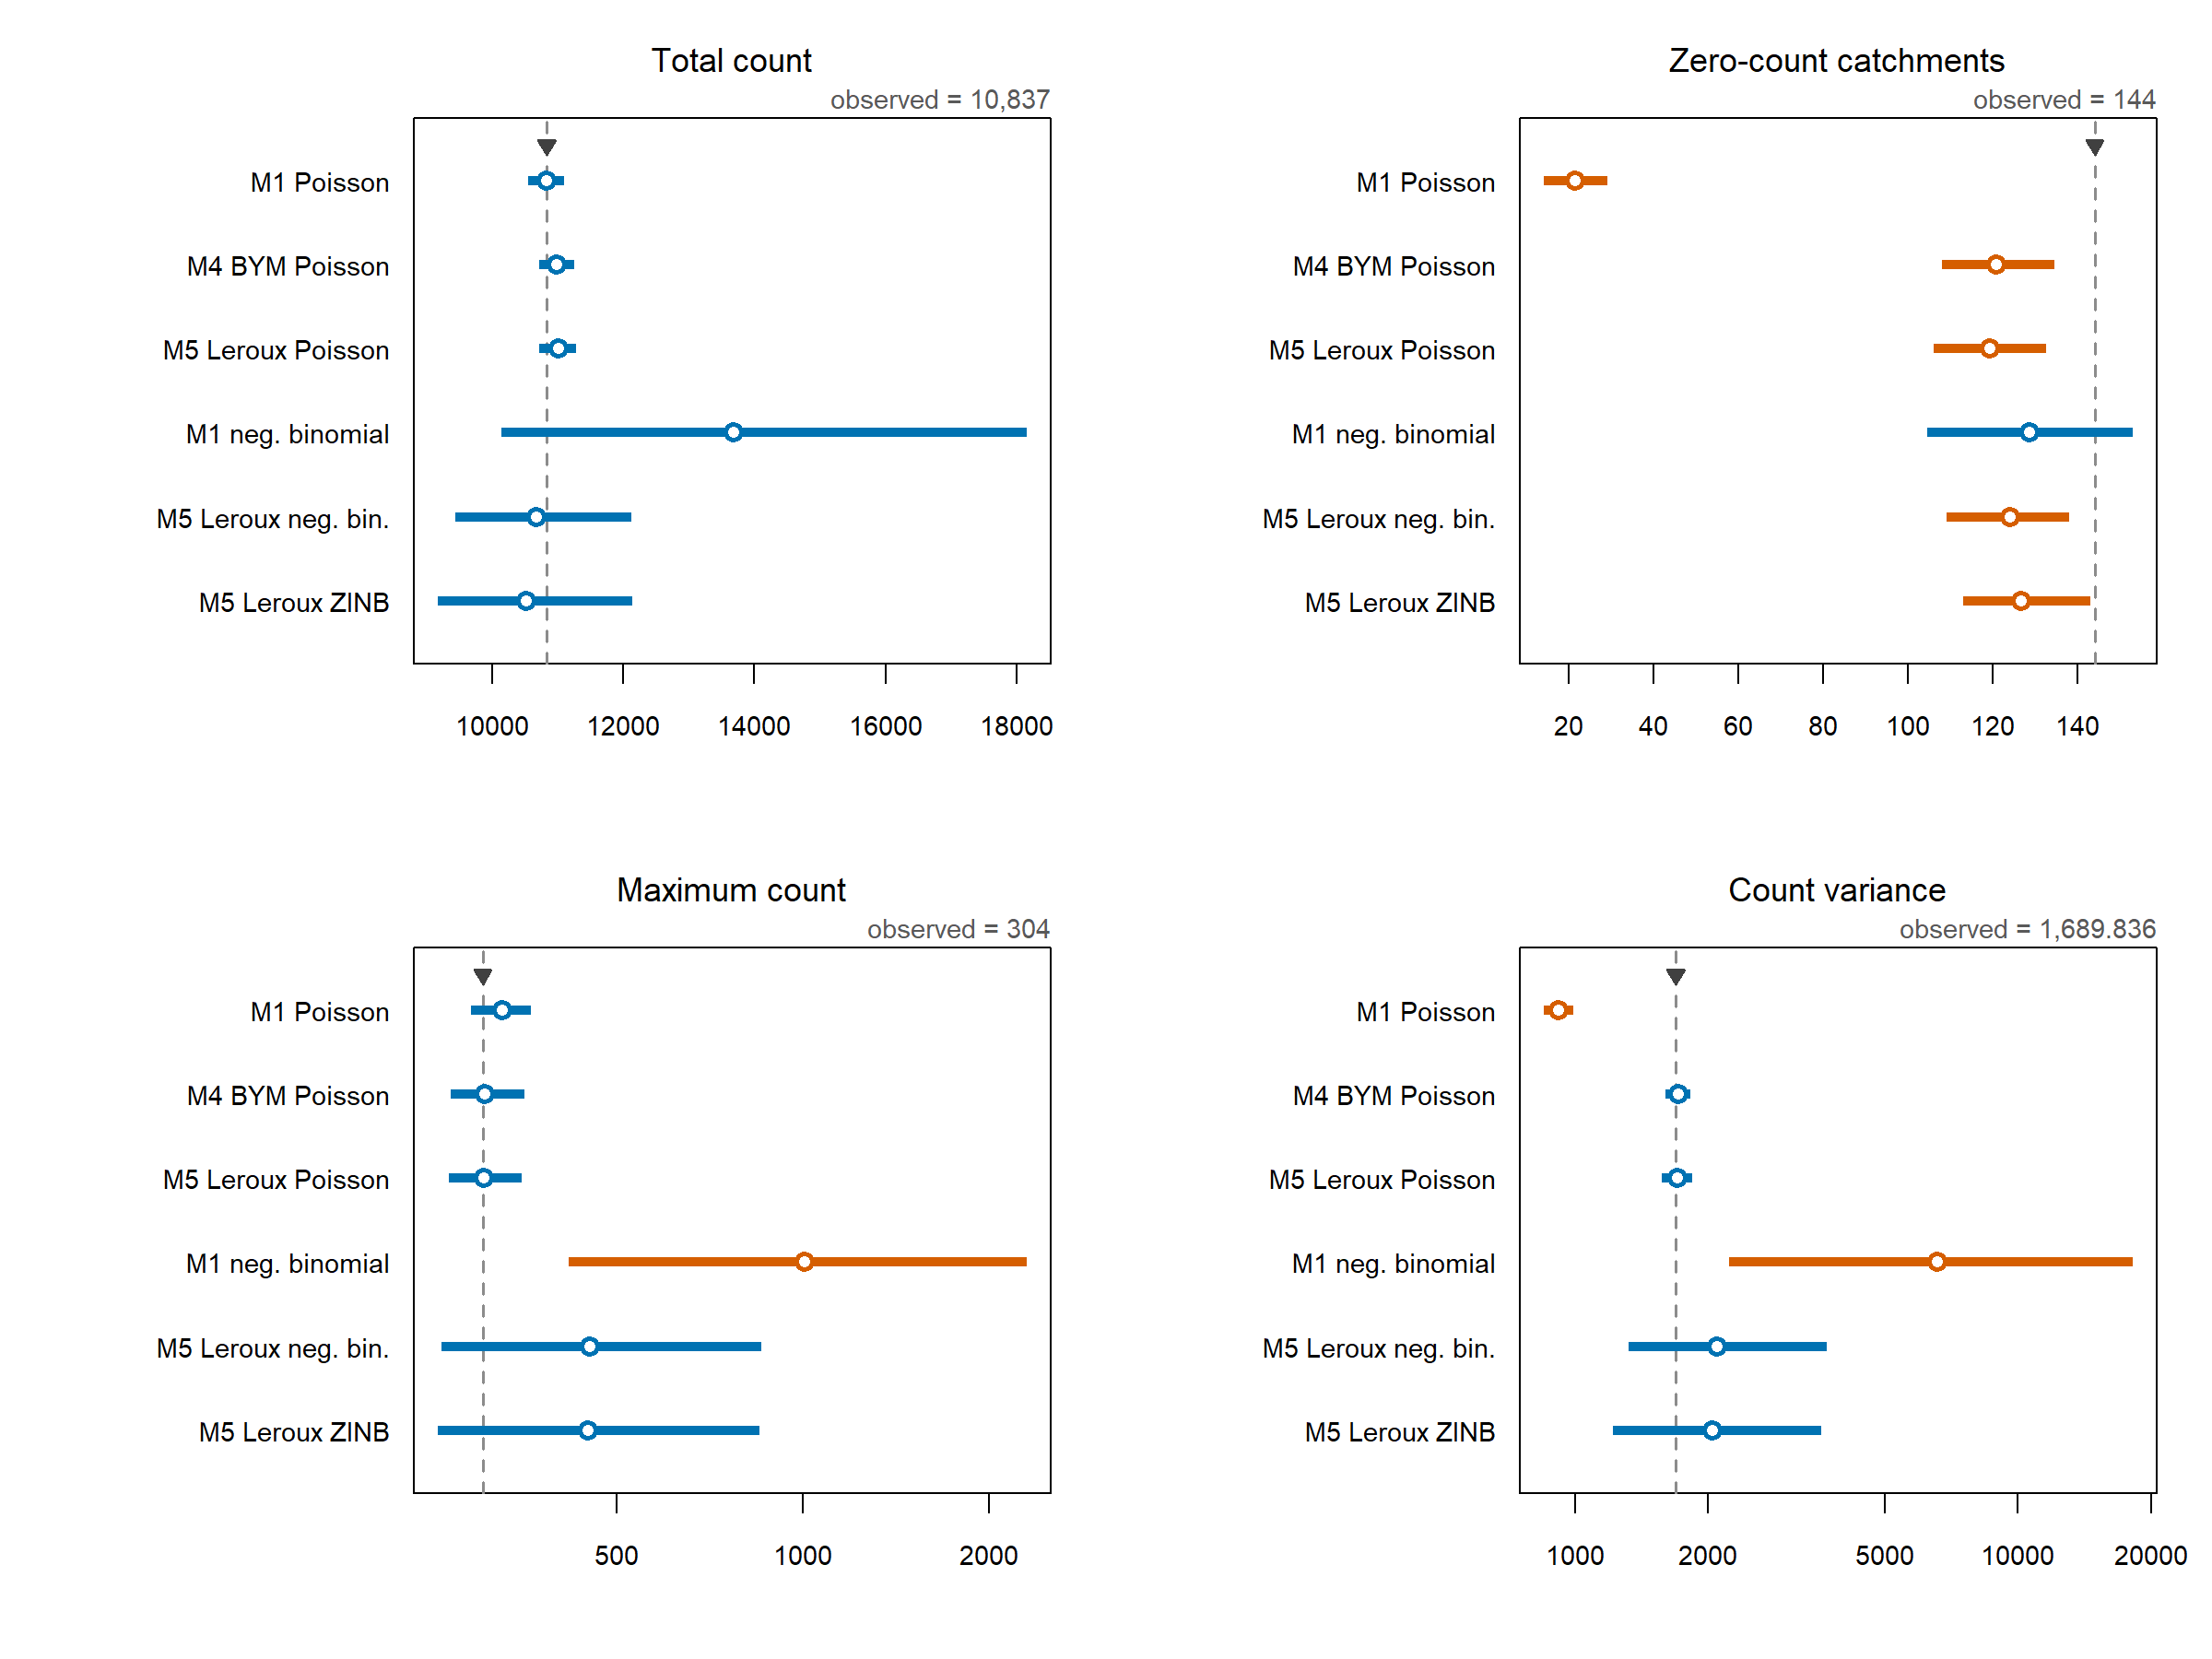
\includegraphics[width=\textwidth]{FigA3_posterior_predictive_checks.png}
\caption{Posterior predictive checks. For each model and statistic, the circle is the mean and the bar the 95\% interval of the statistic over 500 datasets replicated from the posterior; the dashed line and triangle mark the observed value. Intervals that contain the observed value are shown in blue, those that do not in vermillion.}\label{figA3}
\end{figure}

\subsection{Spatial support and the slope-scale control on landslide occurrence}\label{secA6}

The models explain the number of mapped landslides per catchment; they do not model where, within a catchment, an individual slope fails. Mean catchment slope therefore enters as a descriptor of the catchment as a whole, i.e.\ of its bulk steepness, which reflects landscape state, incision and relief and scales with landslide erosion at the catchment level \citep{Montgomery2002, Larsen2012}, and not as a proxy for the critical slope angle at which individual landslides initiate. The analyses in this section test whether aggregating slope to catchment means masks the slope-scale control, and quantify how the between-catchment slope effect relates to it.

\textit{Methods.} (i) The pixel-level variance of slope over the study area was decomposed into a between-catchment component, the area-weighted variance of the catchment means, and a within-catchment component, the area-weighted mean of the within-catchment variances. (ii) The slope of the 12.5~m cell containing each landslide crown was expressed as a percentile of the slope distribution of its own catchment; in the absence of any within-catchment preference for steeper terrain, these percentiles would be uniformly distributed. (iii) The slope-scale response $f(s)$ was estimated from within-catchment contrasts only. Each catchment $c$ was divided into 1$^{\circ}$ slope classes $b$ (0--70$^{\circ}$, steeper cells pooled into the last class), with area $A_{cb}$ and landslide count $n_{cb}$, and
\begin{equation}
n_{cb} \sim \mathrm{Poisson}\left(A_{cb}\, \exp\left[\alpha_c + f(s_b)\right]\right),
\end{equation}
where $\alpha_c$ is a fixed effect for each catchment and $f$ a natural cubic spline with five degrees of freedom, fitted to the 382 catchments that contain at least one landslide. Because every catchment has its own intercept, $f$ is informed only by how landslides are distributed over slope classes inside catchments, and not by how many landslides each catchment has. (iv) The catchment-level expectation implied by a purely slope-scale control was obtained by integrating $f$ over every cell of each catchment,
\begin{equation}\label{eq:Sc}
S_c = \log\left(\frac{1}{A_c}\sum_{b} A_{cb}\, e^{f(s_b)}\right),
\end{equation}
which is the change of support that is consistent with a count response and differs from $f$ evaluated at the mean slope by Jensen's inequality. (v) M1, M4 and M5 were refitted with $S_c$ in place of mean slope, and with $S_c$ added to the offset, so that slope acts only through the slope-scale response. (vi) As a sensitivity analysis on the aggregation function, the models were also refitted with mean slope replaced by the 90th percentile of within-catchment slope, by the proportion of catchment area steeper than 20, 25 and 30$^{\circ}$, a coarse analogue of a restriction to potential process areas \citep{steger2026dynamic}, and with the within-catchment standard deviation of slope added to the mean.

\textit{Results.} Of the pixel-level variance of slope, 67.7\% lies within catchments and 32.3\% between them, so aggregation to catchment means discards about two thirds of the slope information. Landslides prefer the steeper parts of their catchments: the median crown lies at the 64th percentile of the slope distribution of its catchment, 3.6$^{\circ}$ steeper than the catchment mean, and 17.4\% of crowns lie above the 90th percentile of their catchment, against 10\% expected without preference (Fig.~\ref{figA4}b).

The within-catchment response $f(s)$ increases monotonically and is close to log-linear between about 5 and 45$^{\circ}$; the relative intensity rises about eightfold between 2.5 and 60$^{\circ}$ (Fig.~\ref{figA4}a), and the Pearson dispersion of the within-catchment model is 1.06. The pooled frequency ratio, which ignores catchment membership, exaggerates the contrast between gentle and steep terrain relative to $f(s)$, because gently sloping cells lie preferentially in less active catchments. Because $f$ is nearly log-linear, $S_c$ is almost a linear function of mean slope ($r = 0.982$), with a Jensen gap between $-0.06$ and $+0.13$ on the log scale. Replacing mean slope by $S_c$ leaves the models essentially unchanged: in M5, DIC is 2568 against 2572, $\rho$ is 0.887 against 0.894, and the latent field correlates at 0.995 with that of the main specification (Table~\ref{tabA6}). Aggregation by the catchment mean therefore does not mask the slope-scale control in a way that affects the modelled counts or the latent spatial structure.

On its original scale, the coefficient of $S_c$ would be close to 1 if catchment landslide activity reflected only the summed slope-scale response. It is 3.2 (95\% credible interval 2.4--3.9) in M5, 2.6 (2.0--3.2) in M4 and 2.4 (2.3--2.5) in M1. The between-catchment association of steepness with landslide activity is thus about three times stronger than the slope-scale response implies, and the slope coefficients of the main models are between-catchment, i.e.\ ecological, associations that should not be interpreted as slope-scale effects. When slope acts only through the slope-scale response ($S_c$ in the offset), the Leroux latent field absorbs the remainder: its variance increases from 2.51 to 2.66 and $\rho$ from 0.894 to 0.927. The excess between-catchment association is therefore spatially structured, consistent with catchment steepness standing for correlated catchment-scale properties such as incision, relief, regolith and hillslope--channel coupling, and possibly also for spatially uneven landslide detection (Sect.~\ref{subsec54}).

The alternative aggregation functions give the same picture (Table~\ref{tabA6}): the M5 latent field correlates at 0.986--0.997 with that of the main specification, $\rho$ ranges from 0.89 to 0.92, and the slope effect remains credibly positive. Adding the within-catchment standard deviation of slope lowers DIC by 10 and leaves the latent field unchanged ($r = 0.992$).

These analyses have three limitations. Crown locations may fall on the scarp, and the DEM (acquired in 2006--2011) partly records post-failure topography; $f(s)$ is assumed to be common to the whole study area; and mean slope and $S_c$ are too strongly correlated ($r = 0.98$) to be interpreted jointly in a single model.

\begin{table*}[h]
\caption{Sensitivity of the models to the aggregation of the slope predictor. Upper block: the catchment-mean slope is replaced by alternative within-catchment summaries computed from the 12.5~m DEM. Lower block: slope enters through $S_c$, the catchment integral of the within-catchment slope response (Sect.~\ref{secA6}). $\sigma^2_u$ and $\rho$: variance and mixing parameter of the Leroux latent field; $r_u$: correlation of the M5 latent field with that of the published specification; $\beta_S$: standardized slope coefficient in M5 with 95\% credible interval.}\label{tabA6}
\footnotesize
\begin{tabular}{@{}lrrrrrrrl@{}}
\toprule
 & M1 & M4 & \multicolumn{6}{c}{M5-Leroux} \\
\cmidrule(lr){4-9}
Slope predictor & DIC & DIC & DIC & MI & $\sigma^2_u$ & $\rho$ & $r_u$ & $\beta_S$ \\
\midrule
Mean slope (published) & 10,941 & 2,551 & 2,572 & -0.172 & 2.51 & 0.894 & 1.000 & 0.84 [0.63, 1.05] \\
90th percentile & 11,411 & 2,546 & 2,562 & -0.176 & 2.49 & 0.899 & 0.993 & 0.97 [0.75, 1.19] \\
Area fraction $>20^{\circ}$ & 10,579 & 2,551 & 2,573 & -0.170 & 2.53 & 0.892 & 0.997 & 0.77 [0.58, 0.97] \\
Area fraction $>25^{\circ}$ & 11,068 & 2,552 & 2,573 & -0.164 & 2.57 & 0.906 & 0.994 & 0.70 [0.51, 0.90] \\
Area fraction $>30^{\circ}$ & 11,760 & 2,552 & 2,573 & -0.157 & 2.62 & 0.918 & 0.986 & 0.63 [0.44, 0.82] \\
Mean + within-catchment SD & 10,266 & 2,547 & 2,562 & -0.176 & 2.51 & 0.900 & 0.992 & 0.65 [0.41, 0.89] \\
\midrule
$S_c$ (slope-scale integrated) & 10,597 & 2,550 & 2,568 & -0.180 & 2.46 & 0.887 & 0.995 & 0.99 [0.77, 1.22] \\
$S_c$ as fixed offset & 11,774 & 2,551 & 2,574 & -0.143 & 2.66 & 0.927 & 0.950 & -- \\
\bottomrule
\end{tabular}
\end{table*}

\begin{figure*}[h]
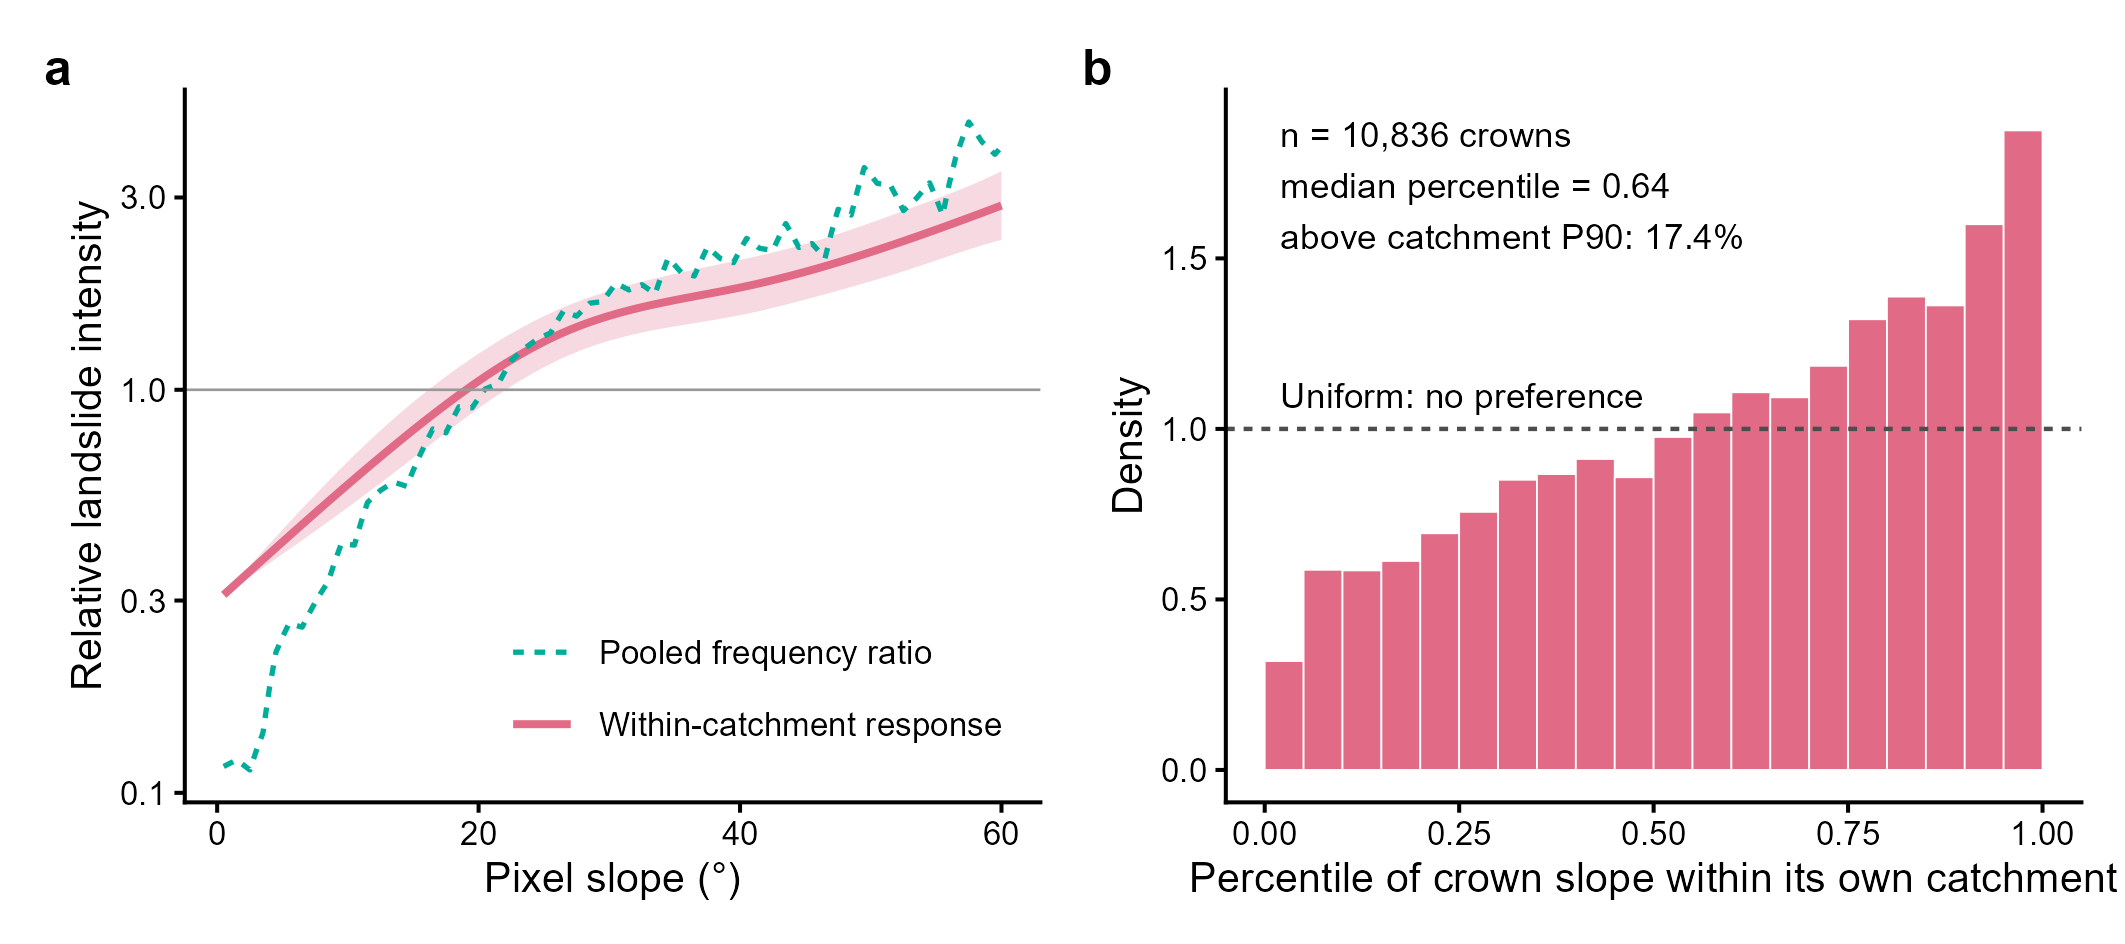
\includegraphics[width=\textwidth]{FigA4_slope_scale_control.png}
\caption{Slope-scale control on landslide occurrence. (a) Relative landslide intensity as a function of 12.5~m cell slope, estimated from within-catchment contrasts (solid line, 95\% confidence band) and as a pooled frequency ratio that ignores catchment membership (dashed line); logarithmic vertical axis. (b) Percentile of the crown-cell slope of each landslide within the slope distribution of its own catchment; the dashed line is the uniform density expected without within-catchment preference.}\label{figA4}
\end{figure*}

\noappendix


\authorcontribution{EA: Conceptualization, Methodology, Software, Formal analysis, Investigation, Writing - Original Draft, Writing - Review \& Editing, and Visualization. LL: Conceptualization, Validation, and Writing - Review \& Editing. OK: Conceptualization, Supervision, Validation, and Writing - Review \& Editing.} %% this section is mandatory

\competinginterests{The authors have no financial or proprietary interests in any material discussed in this article.} %% this section is mandatory even if you declare that no competing interests are present

\begin{acknowledgements}
We gratefully acknowledge the support of the Alexander von Humboldt Foundation for awarding the first author with a Georg Forster Research Fellowship for Experienced Researchers.
\end{acknowledgements}

%% REFERENCES

\bibliographystyle{copernicus}
\bibliography{bibliography}


\end{document}
